\documentclass[twoside]{article}
\usepackage[a4paper]{geometry}
\usepackage{RR}
%\usepackage{hyperref}
\usepackage[american]{babel}
\usepackage[utf8]{inputenc}
\usepackage[T1]{fontenc}
\usepackage{a4wide}

\RRNo{9109}
\RRdate{October 2017}

\RRauthor{
Thomas Herault\thanks[knoxville]{University of Tennessee Knoxville, USA}%
\and Yves Robert\thanks[ens]{Ecole Normale Superieure de Lyon \& INRIA, France}\thanksref{knoxville}%
\and Aurelien Bouteiller\thanksref{knoxville}%
\and Dorian Arnold\thanks[emory]{Emory University, Atlanta, GA, USA}%
\and Kurt B.~Ferreira\thanks[sandia]{Center for Computing Research, Sandia National Laboratory, USA}%
\and George Bosilca\thanksref{knoxville}%
\and Jack Dongarra\thanksref{knoxville}}
%% Ceci apparait sur chaque page paire.
\authorhead{Herault, Robert, Bouteiller, Arnold, Ferreira, Bosilca, Dongarra}

%% FR
\RRtitle{Stratégies de checkpoint coopératives sur plates-formes partagées}

\RRetitle{Optimal Cooperative Checkpointing for Shared High-Performance Computing Platforms
\thanks{Based in part upon work supported by the National Science Foundation under Grant Number 1564133, ``Toward Extreme Scale Fault-Tolerance: Exploration Methods, Comparative Studies and Decision Processes''.}}

\titlehead{Optimal Cooperative Checkpointing for Shared High-Performance Computing Platforms}

\RRresume{Ce rapport s'intéresse aux plates-formes de calcul scientifique partagées, i.e., sur lesquelles s'exécutent simultanément plusieurs classes d'applications. Celles-ci sont en compétition pour l'accès aux ressources d'entrées-sorties, à la fois pour leurs opérations de base et pour prendre leurs checkpoints. Nous proposons un modèle et analysons plusieurs stratégies de prise de checkpoints, à période fixe ou dépendant de l'application, avec ou sans interférence, bloquante ou non. Nous déterminons une borne inférieure sur la fraction de temps nécessairement perdue  
par la plateforme pour toute stratégie de checkpoint/redémarrage, et nous montrons 
expérimentalement que notre  stratégie coopérative obtient des performances très proches de cette borne. Dans notre  stratégie coopérative, les périodes de checkpoint des applications ne sont pas nécessairement celles
calculées par la formule de Young/Daly, car la bande passante 
disponible ne permet pas toujours de les mettre en oeuvre, et certaines applications ont nécessairement une période plus longue (et donc sous-optimale).
Nous donnons les résultats d'un ensemble de simulations menées avec des ensembles 
de paramètres pour les applications et les plates-formes qui correspondent à des scénarios actuels et prospectifs.}

\RRabstract{
In high-performance computing environments, input/output (I/O) from various
sources often contend for scare available bandwidth. Adding to the I/O
operations inherent to the failure-free execution of an application, I/O
from checkpoint/restart (CR) operations (used to ensure progress in the presence
of failures) places an additional burden as it increases I/O contention,
leading to degraded performance.  In this work, we consider a cooperative scheduling policy that optimizes the
overall performance of concurrently executing CR-based applications which share
valuable I/O resources.  First, we provide a theoretical model and then derive a set
of necessary constraints needed to minimize the global \emph{waste} on the
platform.
  Our results demonstrate that the optimal checkpoint interval as defined by
Young/Daly, while providing a sensible metric for a single application, is not
sufficient to optimally address resource contention at the platform scale.  We
therefore show that combining optimal checkpointing periods with I/O scheduling
strategies can provide a significant improvement on the overall application
performance, thereby maximizing platform throughput.
Overall, these results provide critical analysis and direct guidance on checkpointing
large-scale workloads in the presence of competing I/O while minimizing the impact
on application performance.
}

\RRmotcle{résilience, checkpoint, optimisation I/O, stratégie d'ordonnancement.}

\RRkeyword{checkpoint, I/O contention, shared platform, scheduling policy, cooperative checkpoint.}

\RRprojet{ROMA}
\RCGrenoble 



\usepackage[hidelinks]{hyperref}
\usepackage{graphicx}
\usepackage{amsmath,amssymb,amsfonts,amsthm}
\DeclareMathOperator{\lcm}{lcm}
\usepackage{paralist}
\usepackage{color}
\usepackage{xspace}
\usepackage{algorithm}
\usepackage{algorithmicx}
\usepackage{todonotes}
\usepackage{verbatim}
\usepackage{cleveref}

%\addtolength{\textfloatsep}{-1.5em}
%\addtolength{\abovecaptionskip}{-1.25em}

\usepackage{array}
\newcolumntype{L}[1]{>{\raggedright\let\newline\\\arraybackslash\hspace{0pt}}m{#1}}
\newcolumntype{C}[1]{>{\centering\let\newline\\\arraybackslash\hspace{0pt}}m{#1}}
\newcolumntype{R}[1]{>{\raggedleft\let\newline\\\arraybackslash\hspace{0pt}}m{#1}}

\usepackage{gnuplot-lua-tikz}

\newtheorem{example}{Example}
\newtheorem{theorem}{Theorem}

\newcommand*{\email}[1]{\href{mailto:#1}{\nolinkurl{#1}} }
\newcommand{\ie}[0]{\emph{i.e.}\xspace}
\newcommand{\eg}[0]{\emph{e.g.}\xspace}

\newcommand{\muind}{\mu_{\text{ind}}}
\newcommand{\bandtotal}{\beta_{\text{tot}}}
\newcommand{\bandavail}{\beta_{\text{avail}}}
\newcommand{\appset}{{\mathcal A}}
\newcommand{\nbnodesplat}{{\mathcal N}}
\newcommand{\nbapps}{|{\mathcal A}|}
\newcommand{\app}[1]{A_{#1}}
\newcommand{\application}[2]{a_{#1}^{#2}}
\newcommand{\nbapp}[1]{n_{#1}}
\newcommand{\nbnodes}[1]{q_{#1}}
\newcommand{\period}[1]{P_{#1}}
\newcommand{\ckpt}[1]{C_{#1}}
\newcommand{\reco}[1]{R_{#1}}
\newcommand{\size}[1]{\mathit{size}_{#1}}
\newcommand{\wasteapp}[1]{W_{#1}}
\newcommand{\wap}[1]{W_{#1}}
\newcommand{\wapp}[2]{W_{#1}(#2)}
\newcommand{\mtbfplat}{\mu}
\newcommand{\wasteplat}{W}
\newcommand{\ioconstraint}{F}
\newcommand{\lastckpt}[2]{L_{#1}^{#2}}
\newcommand{\wastefct}[2]{W_{#1}(#2)}
\newcommand{\pool}{{\mathcal P}}
\newcommand{\risk}{{\textsc Risk}}
%\newcommand{\todo}[1]{\textit{TBD: [#1]}}
\newcommand{\dca}[1]{\todo[inline]{DCA: #1}}
\newcommand{\kbf}[1]{\todo[inline]{kbf: #1}}

\newcommand{\IOcat}{\textsc{IO-Candidate}\xspace}
\newcommand{\Ckptcat}{\textsc{Ckpt-Candidate}\xspace}
\newcommand{\Catiocat}{\mathcal{C}_{IO}\xspace}
\newcommand{\Catckptcat}{\mathcal{C}_{Ckpt}\xspace}

\newcommand{\nocoop}{\emph{Oblivious}\xspace}
\newcommand{\fifoblock}{\emph{Ordered}\xspace}
\newcommand{\fifononblock}{\emph{Ordered-NB}\xspace}
\newcommand{\leastwaste}{\emph{Least-Waste}\xspace}

\def\propfixed{\nocoop-Fixed\xspace}
\def\propdaly{\nocoop-Daly\xspace}
\def\bfifofixed{\fifoblock-Fixed\xspace}
\def\bfifodaly{\fifoblock-Daly\xspace}
\def\fifofixed{\fifononblock-Fixed\xspace}
\def\fifodaly{\fifononblock-Daly\xspace}
\def\cooperative{\leastwaste}

\begin{document}

\makeRR   % cas d'un rapport de recherche

%% !TEX root =  ipdps18.tex

\section{Introduction}
\label{sec:intro}
% Primary: George & Dorian

%space sharing but not quite
\emph{Space-sharing} high-performance computing (HPC) platforms for the
concurrent execution of multiple parallel applications is the prevalent usage
pattern in today's HPC centers.  In fact, space-sharing in this fashion is more
common than \emph{capability} workloads that span the entire
platform~\cite{Weidner2016}. Furthermore, while computational nodes are
dedicated to a particular application instance, the interconnect links and
storage partition are typically shared amongst application instances. Therefore,
without careful consideration, network and storage contention can reduce
individual application and overall system performance \todo{kbf: CITE "There goes the
neighborhood"?}.

On these platforms, checkpoint/restart (CR) is the most common strategy
employed to protect applications from underlying faults and failures.
Generally, CR periodically outputs snapshots (i.e. checkpoints) of its global,
distributed state to some stable storage device. When an application failure
occurs, the last stored checkpoint is retrieved and used to restart the
application.  Typically, concurrently executing applications independently
decide when to take their own checkpoints.

There are two widely-used approaches to determine when an application should
\emph{commit} a checkpoint: (i)~using a fixed checkpoint period (typically one
or a few hours) for each application; and (ii)~using platform and
application-specific metrics to determine its optimal checkpoint period. In the
second approach, the well-known Young/Daly formula~\cite{young74,daly04} yields
an application optimal checkpoint period, $\sqrt{2 \mu C}$ seconds, where $C$
is the time to commit a checkpoint and $\mu$ the application Mean Time Between
Failures (MTBF) of the platform.  In most cases, $\mu = \frac{\muind}{q}$,
where $q$ is the number of processors enrolled by the application and $\muind$
is the MTBF of an individual processor~\cite{springer-monograph}. Therefore,
both $\mu$ and $C$ in the Young/Daly formula are application-dependent, and
optimal periods can be quite different over the application spectrum.

Independent CR of concurrent application instances can incur significant
resource wastage, because they lead to an inefficient usage of an already
scarce resource, namely available I/O bandwidth\todo{kbf: CITE R. Ross SOP
paper?}.  There are two major reasons for this:

\begin{enumerate}
        
\item \emph{Application-CR I/O contention}: On many systems, the I/O subsystem
does not have enough available usable bandwidth to meet the requirements of
the concurrent application workloads\todo{kbf: CITE R. Ross SOP paper?}. This
congestion is expected to worsen going forward with the emergence of many data
intensive workloads in HPC\todo{kbf: CITE}.  Let $\bandtotal$ be the total
filesystem I/O bandwidth.  Concurrently executing applications typically
perform regular (non-CR) I/O operations throughout their execution, so that
only a fraction $\bandavail$ of the total bandwidth remains available for
checkpoints.  This fraction may be insufficient, particularly when some
applications perform intensive non-checkpoint I/O and others may write very
large checkpoints.
  % $\bandtotal$ of a well-provisioned platform should allow for efficient CR
  % I/O activities.

\item \emph{CR-CR I/O contention}: Most importantly, there is a high
probability of overlapping CR activity amongst concurrent application
instances.  Consider the simple case where two applications of same size
checkpoint simultaneously a file of the same size. Each will be assigned half
the fraction $\bandavail$ to checkpoint, therefore the commits will take twice
as long. Such interferences can severely decrease application efficiency and
overall platform throughput (e.g., when the expected checkpoint commit time
used to compute the optimal checkpoint interval differs from the actual
checkpoint commit time)\todo{footnote?}.

\end{enumerate}

In this work, we develop and investigate a cooperative CR scheduling strategy
for concurrently executing HPC applications.  Our objective is to assess the
impact of such interferences and to design scheduling algorithms that optimize
I/O bandwidth availability for CR activity.  Using these cooperative
algorithms, applications checkpoint sequentially, with a dynamic,
priority-dependent frequency dictated by a cooperative scheduler.  When enough
I/O bandwidth is available, each application checkpoints with its optimal,
Young/Daly, period.  However, when I/O bandwidth is scarce, our scheduling
algorithm provides an optimal checkpoint period that maximizes overall platform
throughput. This cooperative checkpoint process is calculated such that there
is no I/O interference and minimal re-work to be done when failures occur.

Therefore, the main contributions of this paper are the following:

\begin{itemize}

\item Development of a model allowing for the quantification of
the I/O interference of checkpointing applications sharing a common underlying I/O
substrate.

\item Investigation of the costs of various I/O-aware scheduling
strategies through both steady-state analysis as well as detailed simulations.

\item A detailed survey of a number scheduling strategies: from oblivious
algorithms similar to  those currently deployed on many large-scale platforms,
to ones which exploit application knowledge in an effort to  minimize the total
system waste by scheduling the application with the most critical I/O needs.

\end{itemize}

% - a model to predict the shared I/O impact on multiple applications scenarios
% - I/O scheduling algorithms for non-cooperative application scheduling
%   - non-cooperative I/O scheduling: apps are selected to fill the gaps based on processor count (traditional approach)
%   - blocking FIFO I/O scheduling: favor one of the I/O application
%   - non-blocking FIFO I/O scheduling: same as above but the cost of the queueing the app is now independent of the interference pattern
%   - least-waste algorithm: select the app that will minimize the system waste (I/O or C/R candidate)
% - steady state analysis
% - simulation
% - results

The rest of the paper is organized as follows. Our model is described in
\Cref{sec:model}, followed by a description of the various scheduling
strategies in \Cref{sec:algorithms}. \Cref{sec:lowerbound} presents a
theoretical analysis of the model under a steady-state scenario, and provides a
lower bound of the optimal platform waste. \Cref{sec:simulator} describes the
discrete event simulator used to quantitatively compare the different
scheduling strategies.  \Cref{sec:results} presents the results of the
simulation, providing guidance on the necessary I/O bandwidth for  current and
future systems. This work concludes with related works described in \Cref{sec:related},
followed by a summary and future directions outlined in \Cref{sec:conclusion}.

% - Section~\ref{sec:model} describe the scenario under investigation
% - Section~\ref{sec:algorithms} describe the different I/O scheduling
%   algorithms that we plan to analyze, including one that is highly related to
%   the default scheduling on most HPC platforms
% - Section~\ref{sec:lowerbound} describe a theoretical scenario that allow us
%   to derive the lower-bound
% - Section~\ref{sec:simulator} describe the simulator used to validate the
%   results
% - Section~\ref{sec:results} present the results
% - Section~\ref{sec:related} depicts the related work field
% - Section~\ref{sec:conclusion} conclude

% !TEX root =  ipdps18.tex

\section{Introduction}
\label{sec:intro}
% Primary: George & Dorian

%space sharing but not quite
\emph{Space-sharing} high-performance computing (HPC) platforms for the
concurrent execution of multiple parallel applications is the prevalent usage
pattern in today's HPC centers.  In fact, space-sharing in this fashion is more
common than \emph{capability} workloads that span the entire
platform~\cite{Weidner2016}. Furthermore, while computational nodes are
dedicated to a particular application instance, the interconnect links and
storage partition are typically shared amongst application instances.
Therefore, without careful consideration, network and storage contention can
reduce individual application and overall system
performance~\cite{Bhatele:2013:Neighborhood}.

On these platforms, checkpoint/restart (CR) is the most common strategy
employed to protect applications from underlying faults and failures.
Generally, CR periodically outputs snapshots (\ie checkpoints) of its global,
distributed state to some stable storage device. When an application failure
occurs, the last stored checkpoint is retrieved and used to restart the
application.  Typically, concurrently executing applications independently
decide when to take their own checkpoints.

There are two widely-used approaches to determine when an application should
\emph{commit} a checkpoint: (i)~using a fixed checkpoint period (typically one
or a few hours) for each application; and (ii)~using platform and
application-specific metrics to determine its optimal checkpoint period. In the
second approach, the well-known Young/Daly formula~\cite{young74,daly04} yields
an application optimal checkpoint period, $\sqrt{2 \mu C}$ seconds, where $C$
is the time to commit a checkpoint and $\mu$ the application Mean Time Between
Failures (MTBF) of the platform.  In most cases, $\mu = \frac{\muind}{q}$,
where $q$ is the number of processors enrolled by the application and $\muind$
is the MTBF of an individual processor~\cite{springer-monograph}. Therefore,
both $\mu$ and $C$ in the Young/Daly formula are application-dependent, and
optimal periods can be quite different over the application spectrum.

Independent CR of concurrent application instances can incur significant
resource wastage, because they lead to an inefficient usage of an already
scarce resource, namely available I/O bandwidth~\cite{Luu:2015:Multiplatform}.
There are two major reasons for this:

\begin{compactitem}
        
\item \emph{Application-CR I/O contention}: On many systems, the I/O subsystem
does not have enough available usable bandwidth to meet the requirements of the
concurrent application workloads~\cite{Luu:2015:Multiplatform}. This congestion
is expected to worsen going forward with the increased prevelance of data
intensive workflows in HPC.  Let $\bandtotal$ be the total filesystem I/O
bandwidth.  Concurrently executing applications typically perform regular
(non-CR) I/O operations throughout their execution, so that only a fraction
$\bandavail$ of the total bandwidth remains available for checkpoints.  This
fraction may be insufficient, particularly when some applications perform
intensive non-checkpoint I/O and others may write very large checkpoints.
  % $\bandtotal$ of a well-provisioned platform should allow for efficient CR
  % I/O activities.

\item \emph{CR-CR I/O contention}: Most importantly, there is a high
probability of overlapping CR activity amongst concurrent application
instances.  Consider the simple case where two applications of same size
checkpoint simultaneously a file of the same size. Each will be assigned half
the fraction $\bandavail$ to checkpoint, therefore the commits will take twice
as long. Such interferences can severely decrease application efficiency and
overall platform throughput\footnote{When the expected checkpoint commit time
used to compute the optimal checkpoint interval differs from the actual
checkpoint commit time, effciency will decrease.}.

\end{compactitem}

In this work, we develop and investigate a cooperative CR scheduling strategy
for concurrently executing HPC applications.  Our objective is to assess the
impact of such interferences, and to design scheduling algorithms that optimize
I/O bandwidth availability for CR activity.  Using these cooperative
algorithms, applications checkpoint sequentially, with a dynamic,
priority-dependent frequency dictated by a cooperative scheduler.  When enough
I/O bandwidth is available, each application checkpoints with its optimal,
Young/Daly, period.  However, when I/O bandwidth is scarce, our scheduling
algorithm provides an optimal checkpoint period that maximizes overall platform
throughput. This cooperative checkpoint process is calculated such that there
is no I/O interference and minimal re-work to be done when failures occur.

Therefore, the main contributions of this paper are the following:

\begin{itemize}

\item Development of a model allowing for the quantification of
the I/O interference of checkpointing applications sharing a common underlying I/O
substrate.

\item Investigation of the costs of various I/O-aware scheduling
strategies through both steady-state analysis as well as detailed simulations.

\item A detailed survey of a number scheduling strategies: from oblivious
algorithms similar to  those currently deployed on many large-scale platforms,
to ones which exploit application knowledge in an effort to  minimize the total
system waste by scheduling the application with the most critical I/O needs.

\end{itemize}

% - a model to predict the shared I/O impact on multiple applications scenarios
% - I/O scheduling algorithms for non-cooperative application scheduling
%   - non-cooperative I/O scheduling: apps are selected to fill the gaps based on processor count (traditional approach)
%   - blocking FIFO I/O scheduling: favor one of the I/O application
%   - non-blocking FIFO I/O scheduling: same as above but the cost of the queueing the app is now independent of the interference pattern
%   - least-waste algorithm: select the app that will minimize the system waste (I/O or C/R candidate)
% - steady state analysis
% - simulation
% - results

The rest of the paper is organized as follows. Our model is described in
\Cref{sec:model}, followed by a description of the various scheduling
strategies in \Cref{sec:algorithms}. \Cref{sec:lowerbound} presents a
theoretical analysis of the model under a steady-state scenario, and provides a
lower bound of the optimal platform waste. \Cref{sec:simulator} describes the
discrete event simulator used to quantitatively compare the different
scheduling strategies.  \Cref{sec:results} presents the results of the
simulation, providing guidance on the necessary I/O bandwidth for  current and
future systems. This work concludes with related works described in \Cref{sec:related},
followed by a summary and future directions outlined in \Cref{sec:conclusion}.

% - Section~\ref{sec:model} describe the scenario under investigation
% - Section~\ref{sec:algorithms} describe the different I/O scheduling
%   algorithms that we plan to analyze, including one that is highly related to
%   the default scheduling on most HPC platforms
% - Section~\ref{sec:lowerbound} describe a theoretical scenario that allow us
%   to derive the lower-bound
% - Section~\ref{sec:simulator} describe the simulator used to validate the
%   results
% - Section~\ref{sec:results} present the results
% - Section~\ref{sec:related} depicts the related work field
% - Section~\ref{sec:conclusion} conclude


%% !TEX root =  ipdps18.tex

\section{Model}
\label{sec:model}
% Primary: Yves

%\todo[inline]{Question: how can we consider applications with finite time, initial
%  input and final output? Current idea is to distribute complete
%  volume of I/O over wall time, then take a single fake schedule that
%  assign resources to the apps following a distribution, and say 'it
%  shouldn't be far from finite apps being scheduled eagerly over
%  finite resource for a long time, in average'.}

\paragraph{Computational Platform Model}
In this work, we consider a shared platform that comprises a set of computational
nodes, storage resources in the form of a parallel file system (PFS), and a network
that interconnects the nodes as well as the storage resources. Applications are
scheduled on the platform by a job scheduler such that computational nodes are
space-shared (dedicated) amongst concurrent application instances. However, the I/O
subsystem is time-shared (contended) amongst the application instances, \ie multiple
applications performing I/O simultaneously can result in a per-application reduction
in commit speed. Without loss of generality, we consider a straightforward linear
interference model in which the global throughput remains constant and is evenly
shared among contending applications. (A more adversarial interference models could
be substituted.)

\paragraph{Application Workload Model}
Applications can vary in size (number of computational nodes), duration, memory
footprint and I/O requirements.  \emph{Application I/O} entails loading an input file
at startup, performing regular I/O operations during their main execution phase and
storing an output file at completion. Because applications are long-running
(typically, several hours or days) and the platform is failure-prone, applications
are protected using coordinated CR that incurs periodic \emph{CR I/O}.

To model these behavioral variations with minimal parameters, we make the following
simplifying assumptions (that we validate in the experimental section):
\begin{compactitem}
\item There is a large number of applications, but only a small number of application
  classes, \ie, sets of applications with similar sizes, durations, footprints and
  I/O requirements;
\item Other than initialization and finalization I/O, an application's regular
  (non-CR) I/O operations are evenly distributed over its makespan.
\item Job makespans are precisely known a priori. This allow us to ignore all other
  sources of job disturbance except C/R overheads.
\end{compactitem}
We used specific numbers and characteristics of application classes based on real
benchmark data, such as the APEX benchmark on the Cielo platform~\cite{apex2016}.  To
avoid the side effects induced by hundreds of completely identical application
instances, we use normal distributions for job durations with mean equal to original
APEX value and small (10\%) standard deviation.

\paragraph{Checkpoint Period and I/O Interference}

Both application computation and CR generate I/O requests, and both classes of I/O
activity are scheduled using the same algorithm (Section~\ref{sec:algorithms}). As
described above, steady-state application I/O is regular. However, CR I/O
periodicity, $P$, depends
upon the CR policy being used.  In our model, applications either checkpoint using an
application-defined periodicity or using Young and
Daly's~\cite{young74,daly04} optimal checkpoint period. The latter interval is
computed by, $T=\sqrt{2 C \mu}$, where $C$ is the duration of the checkpoint
transfer, and $\mu$ is the application mean time between failures (MTBF).
$\mu = \frac{\muind}{q}$, where $q$ is the number of processors enrolled by the
application and $\muind$ is the MTBF of an individual
processor~\cite{springer-monograph}.  The parameters in this formula are dependent
upon application features (checkpoint dataset size) and platform features (system
reliability and I/O bandwidth).

Traditionally, when an application, $\app{i}$, completes a checkpoint, its next
checkpoint is scheduled to happen in at least $\period{i}-\ckpt{i}$ (and the first
checkpoint is set at date $\period{i}$).  With potential CR I/O interference,
determining the appropriate checkpointing period can be challenging.
% The observed duration of checkpoints varies depending on how much interference
% happen, on average.
Additionally, I/O scheduling algorithms that try to mitigate I/O interference can
impose further CR I/O delays.  In other words, the traditional strategy of scheduling
subsequent checkpoints at $\period{i}-\ckpt{i}$ yields the desired checkpointing
period $\period{i}$ only in interference-free scenarios. CR I/O delays (induced by
interferences or scheduling delays) dilate the checkpoint duration to $C_{dilated}$,
and the effective period differs from the desired period by the difference
$C_{dilated}-\ckpt{i}$.  (In Section~\ref{sec:algorithms}, we discuss how each I/O
scheduling algorithm accommodates this discrepancy.)

%TODO: do we want to talk about that, if only to say we don't care?
%  {we may want to separate Input+recovery from output+checkpoint (bidirectional channels)}
%  {answer: we could but not sure it is 100\% independent; and it would complicate things without changing the story.}


\paragraph{Job Scheduling Model}
To evaluate the scheduling policies, we consider a finite segment, typically lasting
a small number of days, of a representative schedule where the number of application
instances (jobs) in each class remains approximately constant at every instant. Of
course, with different job execution times, we cannot enforce a fixed proportion of
each application class at every instant. However, we ensure the proper proportion is
enforced in average throughout the schedule execution. Similarly, we enforce that at
every instant during the finite segment, at least 98\% of the nodes are enrolled for
the execution. This allows us to compare actual (simulated) performance with the
theoretical performance of a co-scheduling policy that optimizes the steady-state I/O
behavior of the job portfolio, assuming that all processors are used. We shuffle and
simultaneously present all jobs to the scheduler, which uses a simple, greedy
first-fit algorithm.  We resubmit failed jobs with a new wall-time equal to the
fraction that remained when the last checkpoint was committed. Input I/O becomes
recovery I/O; output I/O is unmodified.

\paragraph{The Formal Model}
We consider a set $\appset$ of $\nbapps$ applications classes
$\app{1}, \ldots \app{\nbapps}$ that execute concurrently on a platform with
$\nbnodesplat$ nodes. Application class $\app{i}$ specifies:
\begin{compactitem}
\item $\nbapp{i}$: the number of applications in $\app{i}$,
\item $\nbnodes{i}$: the number of nodes used by each application in $\app{i}$,
\item $\period{i}$: the checkpoint period of each application in $\app{i}$, and
\item $\ckpt{i}$ and $\reco{i}$: the checkpoint and recovery durations for each application in $\app{i}$ when there is no interference with other I/O operations.
\end{compactitem}
%
%$\nbapp{i}$ applications that each use
%$\nbnodes{i}$ nodes, and checkpoints
%periodically with period $\period{i}$, in a time $\ckpt{i}$ when there
%is no interference with other I/O operation.
%
At every instant, we schedule as many applications as possible.
Application that are subject to failures are restarted at the head of
the scheduling queue, so that (given that in most cases only one
node has failed and can be replaced by a hot spare) it may restart
immediately on essentially the same compute nodes it previously occupied.

% This is not true in general
% For simplicity, in the theoretical analysis, we ignore the hot spare
% nodes (presumably an insignificant fraction of the total),
% and assume that $\sum_{i}\nbapp{i} \nbnodes{i} = \nbnodesplat$,
% where $\nbnodesplat$ is the total number of nodes in the platform.

%\todo[inline]{the portfolio of available and scheduled applications are not the same, no reason for available applications to match that constraints on node count, only on scheduled ones. }

%Consider a large-scale platform with several applications executing
%concurrently. All these applications routinely perform I/O operations
%throughout their execution. The average fraction of I/O bandwidth that
%remains available can be used for checkpointing. Ideally, each application $A_{i}$
%should checkpoint, during a time $C_{i}$ ,
%every $P_{i}$ units of time. Here $P_{i}$ is the length of the
%optimal checkpointing period given by the Young/Daly formula~\cite{young74,daly04}:
%$$P_{i} = \sqrt{2 \mu_{i} C_{i}}$$
%where $\mu_{i}$ is the application MTBF, which is inversely
%proportional to the number of processors enrolled in its execution.
%
%However, with each application having a different $P_{i}$, lasting and
%starting for and at arbitrary times (a behavior we call
%uncooperative), nothing prevents the checkpoint of an application to
%occur while another competitively does I/O (because of its normal
%application behavior, or because of a checkpoint). Because this
%introduces interferences between I/O (\cite{interference}), the time
%to complete both the checkpoint of the first application and the
%competing I/O of the second are adversely impacted. When many
%applications execute an I/O operation competitively, all of them can
%be impacted, reducing the efficiency of each.
%
%Moreover, checkpointing each application with optimal period $P_{i}$
%is possible only if enough I/O bandwidth is available. If this is the
%case, the impact of failures is kept to a minimum using Daly's period
%for each application.  However, if I/O bandwidth is limited, either in
%the absolute (imbalanced hardware design) or in the current
%co-execution (because a few applications need to consume a large
%fraction of bandwidth to progress), applications have to checkpoint
%less frequently.  All of them? if not, which ones? what are the
%optimal checkpointing periods in this context of co-scheduling with a
%given bound on available I/O bandwidth, and how to schedule the
%checkpoints in order to minimize interferences and optimize resource
%spent doing I/O? This paper answers these important questions.

% !TEX root =  ipdps18.tex

\section{Model}
\label{sec:model}
% Primary: Yves

\paragraph*{Computational Platform Model}

In this work, we consider a shared platform comprised of computational
nodes, storage resources in the form of a parallel file system (PFS), and a network
that interconnects the nodes and storage resources. Applications are
scheduled on the platform by a job scheduler such that computational nodes are
space-shared (dedicated) amongst concurrent application instances. However, the I/O
subsystem is time-shared (contended) amongst application instances  (\ie multiple
applications performing I/O simultaneously result in a per-application reduction
in commit speed). Without loss of generality, we consider a straightforward linear
interference model in which the global throughput remains constant and is evenly
shared among contending applications, proportional to their size\footnote{A more
adversarial interference model can be substituted, if needed.}.

\paragraph*{Application Workload Model}

Applications can vary in size (computational node count), duration, memory
footprint and I/O requirements.  \emph{Application I/O} entails loading an input file
at startup, performing regular I/O operations during their main execution phase and
storing an output file at completion. Because applications are long-running,
(typically, several hours or days) and the platform is failure-prone, applications
are protected using coordinated CR that incurs periodic \emph{CR I/O}.

To model these behavioral variations with minimal parameters, we make the following
simplifying assumptions:
\begin{compactitem}
\item There is a large number of applications, but only a small number of application
  classes, \ie, sets of applications with similar sizes, durations, footprints and
  I/O needs;
\item Excluding initialization and finalization I/O, an application's regular
  (non-CR) I/O operations are evenly distributed over its makespan;
\item Job makespans are known a priori. This allows us to ignore all other
  sources of job disturbance except C/R overheads.
\end{compactitem}

We use specific numbers and characteristics of application classes based on
documented production workloads, such as those provided in the APEX workflows report
on the Cielo platform~\cite{apex2016}.  To avoid the side effects induced by
hundreds of completely identical jobs, we use a normal distributions for job
durations with a mean equal to original APEX value and small (20\%) standard
deviation.  In the rest of the paper, we use the term \emph{job} to denote
a specific application instance, and \emph{application class} to denote a set
of applications with similar characteristics.

\paragraph*{Checkpoint Period and I/O Interference}

Both application computation and CR generate I/O requests.  In both cases, activity
is scheduled using an I/O scheduling algorithm (see \Cref{sec:algorithms}). As
described above, steady-state application I/O is regular. However, CR I/O
periodicity, $P$, depends upon the CR policy being used.  In our model, applications
either checkpoint using an application-defined periodicity or using Young and
Daly's~\cite{young74,daly04} optimal checkpoint period detailed in
\Cref{sec:intro}. As stated previously, the parameters in this formula are dependent
upon application features (checkpoint dataset size) and platform features (system
reliability and I/O bandwidth).  For fixed, application-defined periods, a common
heuristic is to take a checkpoint every hour -- capping the worst case amount of lost
work at one hour.  In the reminder of this paper we will refer to the two variants as
\emph{Fixed} (with a 1 hour period unless otherwise specified) and \emph{Daly}.




Traditionally, when a job $J_{i}$ of class $\app{i}$ completes a checkpoint, its next
checkpoint is scheduled to happen $\period{i}-\ckpt{i}$ instants later (and the first
checkpoint is set at date $\period{i}$). With potential CR I/O interference,
the checkpoint commit may last longer than $\ckpt{i}$, and setting
the appropriate checkpointing period can be challenging.
Additionally, I/O scheduling algorithms that try to mitigate I/O interference can
impose further CR I/O delays.  In other words, the traditional strategy of scheduling
subsequent checkpoints at $\period{i}-\ckpt{i}$ yields the desired checkpointing
period $\period{i}$ only in interference-free scenarios. CR I/O delays (induced by
interferences or scheduling delays) dilate the checkpoint duration to $C_{dilated}$,
and the effective period differs from the desired period by the difference
$C_{dilated}-\ckpt{i}$.  \Cref{sec:algorithms} discusses how each I/O
scheduling algorithm handles this discrepancy.

\paragraph*{Job Scheduling Model}

To evaluate the scheduling policies, we consider a finite segment, typically
lasting a few days, of a representative schedule where the computing resource
usage by each application instance (job) in each class remains nearly constant.
Of course, with varying job execution times, we cannot enforce a fixed
proportion of each application class at every instant. However, we ensure the
proper proportion is enforced on average throughout the schedule execution.
Similarly, we enforce that at every instant during the finite segment, at least
98\% of the nodes are enrolled for the execution. This allows us to compare
actual (simulated) performance with the theoretical performance of a
co-scheduling policy that optimizes the steady-state I/O behavior of the job
portfolio, assuming that all processors are used. We shuffle and simultaneously
present all jobs to the scheduler, which uses a simple, greedy first-fit
algorithm.  We resubmit failed jobs with a new wall-time equal to the fraction
that remained when the last checkpoint commit started.  In this case, input I/O
becomes recovery I/O; output I/O is unmodified.

\paragraph*{The Formal Model}

We consider a set $\appset$ of $\nbapps$ applications classes
$\app{1}, \ldots \app{\nbapps}$ that execute concurrently on a platform with
$\nbnodesplat$ nodes. Application class $\app{i}$ specifies:
\begin{compactitem}
\item $\nbapp{i}$: the number of jobs in $\app{i}$,
\item $\nbnodes{i}$: the number of nodes used by each job in $\app{i}$,
\item $\period{i}$: the checkpoint period of each job in $\app{i}$, and
\item $\ckpt{i}$ and $\reco{i}$: the checkpoint and recovery durations for each job in $\app{i}$ when there is no interference with other I/O operations.
\end{compactitem}

Jobs inherit their characteristics from their classes. To simplify notations, 
for a job $J_j$, we use $\nbnodes{j}, \period{j}, \ckpt{j}$ and
$\reco{j}$ to denote respectfully the number of nodes, checkpoint
period, and checkpoint and recovery durations of the application class
to which $J_j$ belongs.  We let
$\period{Daly}(J_{j}) = \sqrt{2 \ckpt{j} \mu_{j}}$ be the \emph{Daly
  period}~\cite{young74,daly04} of a job $J_j$, where
$\mu_{j} = \frac{\muind}{\nbnodes{j}}$ and $\muind$ is the MTBF of an
individual processor~\cite{springer-monograph}.  At each instance, we
schedule as many jobs as possible.  Jobs that are subject to failures
are restarted at the head of the scheduling queue, as to restart
immediately on the same compute nodes previously used (in most cases,
only one node has failed and is replaced by a hot spare).



%% !TEX root =  ipdps18.tex

\section{I/O Scheduling Algorithms}\label{sec:algorithms}
% Aurelien & George

In this section, we present the algorithms used to schedule applications
I/O workloads in order to assess and alleviate the effect of concurrent access
to I/O resources. The first algorithm (\nocoop) represents the status-quo
in which applications are scheduled in a non-cooperative manner, which may
incur interference on I/O resource access and wait time. The second
algorithm (\fifoblock) coordinate applications to eliminate interference
between their I/O activities: only one application performs I/O at any given
time while other applications requesting I/O are blocked until their
turn (FIFO) comes. The third algorithm (\fifononblock) is similar, except
that applications that are waiting for the I/O token
continue computing until their turn comes; note that unlike the
blocking algorithms, this optimization requires
application code refactoring. Last, we propose an heuristic
(\leastwaste) that improves on \fifononblock by giving the I/O token
to the application that imposes the least overhead on the system. Before
presenting the algorithms, we further discuss the interactions between
the checkpointing policy, the I/O workloads, and the interferences that the
algorithms have to consider.

%Instead of following a FIFO order to select the next I/O application,
%for each requesting application, the heuristic computes the prospective
%waste incurred by delaying its I/O (considering checkpoint and
%probabilistic recovery costs, idle time, etc.) when selecting another
%application, and selects the one that minimizes the waste increase
%at the current instant.

\subsection{Checkpoint Period and I/O Workload}

Both applications and checkpointing generate I/O requests. I/O requests
are all scheduled using the same algorithm whether they
are generated from an application I/O request or from a CR
request. Note however that unlike application I/O, the checkpointing
volume and frequency is dependent upon scheduling decisions.
Some applications
control their own checkpointing completely, and decide to checkpoint at
fixed time steps or application-defined time intervals.
Young and Daly~\cite{young74,daly04} devised a formula to compute the optimal
checkpoint period, $T=\sqrt{2 C \mu}$, where $C$ is the duration of the
checkpoint transfer, and $\mu$ is the reliability of the platform.
The parameters in this formula are dependent upon application features
(the size of the checkpointed dataset) and platform values (the reliability
of the system and the I/O bandwidth).

In traditional periodic checkpointing, for an application $\app{i}$,
every time a checkpoint completes, the next checkpoint is scheduled to
happen in at least $\period{i}-\ckpt{i}$ (and the first checkpoint is
set at date $\period{i}$). $\period{i}$ can be 1) a \emph{fixed} period,
either hardcoded in the application, or set as an arbitrary platform
global setting, or 2) the \emph{Daly} optimal period for the
application on that platform. Note that in a system where interference
can happen (from competing application I/O or checkpoints), determining
the appropriate checkpointing period can be challenging.
% The observed duration of checkpoints varies depending on how much
% interference happen, on average.
Similarly, when employing I/O scheduling algorithms,
checkpoints may include wait time delay or be postponed to decrease
interference. The traditional strategy of rearming the next checkpoint at
$\period{i}-\ckpt{i}$ yields the desired checkpointing period $\period{i}$
only in interference-free scenarios: when interferences (or scheduling
introduced delays) dilate the checkpoint duration to $C_{dilated}$, the effective
period differs from the desired period by the difference $C_{dilated}-\ckpt{i}$.
The details of how each algorithm accommodates for this discrepancy will
be discussed later.

%TODO: do we want to talk about that, if only to say we don't care?
%  {we may want to separate Input+recovery from output+checkpoint (bidirectional channels)}
%  {answer: we could but not sure it is 100\% independent; and it would complicate things without changing the story.}

\subsection{Non-cooperative \nocoop I/O Scheduling}

In the non-cooperative I/O scheduling \nocoop, applications
fill-up the system based on processor count availability, and their I/O
workload (including checkpointing activities) are not organized by any
comprehensive system. Instead, applications use the Parallel FileSystem (PFS) assuming they
are the sole user, and do not modify their access pattern to accommodate
for possible interferences. In these conditions, it has been observed~\cite{Dorier2014}
that concurrent access
to I/O resources will cause a decrease in the application observed
I/O bandwidth.
% One can imagine multiple cost functions for the effect of that sharing;
When the filesystem is under-provisioned, the overall throughput of the platform
would be maintained when multiple applications concurrently access I/O, and each
application should thereby observe a linear decrease in its own bandwidth. As an
application blocks on the I/O completion before it can continue, the decrease in
observed bandwidth leads to a proportionate increase in I/O time that must be
accounted as waste.

Checkpoints are scheduled accordingly to the normal rearming strategy
(\ie after each checkpoint completion, the next checkpoint is scheduled
to start after $\period{i}-\ckpt{i}$). Given that checkpoints may actually
last longer than $\ckpt{i}$, the resultant period may be longer than
$\period{i}$. This is however consistent with the concept of a
checkpointing strategy that is applied blindly, without consideration
for issues stemming from I/O resource sharing and interferences.

In the \nocoop algorithm, we consider two variants where checkpoints are
tentatively taken at 1) fixed frequency (\propfixed), or 2) at the
Daly frequency (\propdaly).

\subsection{Blocking \fifoblock FIFO I/O Scheduling}

A simple optimization to the aforementioned scheme is to favor one of
the applications' I/O request over all others. While the overall throughput
may remain unchanged (given an efficient PFS implementation), the favored
application completes its I/O workload faster (\ie, at nominal speed
$\ckpt{i}$ for an application of class $\app{i}$).
Applications are selected to perform I/O in the order of their requests,
\ie ,as soon as an application starts blocking on an I/O operation it will
take a place in the back of an  I/O FIFO queue. When the currently
active application completes its I/O, the next application waiting for I/O
is granted access, and starts making progress. We denote this scheme as
\fifoblock.

The advantage of \fifoblock over \nocoop can be seen in a simple workload with two
applications, assuming a favorable linear interference model.
If the two applications simultaneously start an I/O requesting the
transfer of a similar volume $V$ of data, in the \nocoop strategy,
both applications take $2 \times \frac{V}{\bandavail}$ time to complete
their I/O. In the \fifoblock strategy, the first (as serialized when
inserting in the FIFO) application takes only $\frac{V}{\bandavail}$
as it enjoys exclusive access to the PFS, while the second application
waits $\frac{V}{\bandavail}$ before its own I/O starts, but then in turn
also complete at nominal speed $\frac{V}{\bandavail}$, and therefore still
completes in $2 \times \frac{V}{\bandavail}$. Thanks
to reducing I/O interferences, the average I/O completion time
has been reduced for the applications (although fairness has been decreased).

Similarly to the previous strategy, application observed checkpoint
duration may increase past $\ckpt{i}$, no longer because of interference, but now because
of  the time spent waiting for the first place in the I/O scheduling FIFO.
As we have computed above, although the average $C-\ckpt{i}$
difference is lower, for one application it is as large as in the
previous strategy. In any case, again, the checkpointing period will
be, in average, larger than the desired $\period{i}$ period.

In the \fifoblock algorithm, we consider two variants where checkpoints are
tentatively taken at 1) fixed frequency (\bfifofixed), or 2) at the
Daly frequency (\bfifodaly).

\subsection{Non-Blocking \fifononblock FIFO I/O Scheduling}

In the previous strategy, the cost of I/O interferences has been
exchanged for idle time when waiting for the I/O token in a blocking
fashion. If the application developer can refactor the code
to continue computing while awaiting for the I/O request to be granted,
it becomes possible to overlap the idle time with useful computation.
Indeed, checkpointing I/O operations can
be effectively time-shifted, at the risk of increasing the exposure to failures.
 In the \fifononblock algorithm, at the end of the previous checkpoint, a tentative
date for the next checkpoint is set at $t_{req}=t_{now}+\period{i}-\ckpt{i}$.
When the application reaches date $t_{req}$, a non-blocking I/O request
is made and reserves a position in the
I/O queue. The application keeps computing until the
scheduler informs the application that the I/O system is exclusively
available to the application. Then, the application initiates its
I/O (checkpointing, initial input, final output or recovery). When the active application completes
its I/O, the next requesting application (in FIFO order)
become the active I/O application.

When an application is informed that it can use the I/O system to
checkpoint, the checkpointing library or application mechanism
in charge of synchronizing the checkpoints may immediately (or after
a short synchronization) start producing the checkpoint I/O workload
(typical for system-based checkpoint),
or finish the current computing block before allowing the checkpoint
to proceed (typical for user-level checkpoint). In this work, we consider
that this resynchronization cost is negligible with respect to the
checkpoint duration. Should a failure impact that application,
it would restart from the date at which the last checkpoint was taken, and
not at $t_{req}$, which is another improvement when compared to the
\fifoblock and \nocoop algorithms.
%\todo[inline]{If we talk about the positive aspect we might also want to mention the negative one, when a fault trigger during the I/O introduced delay}.

Again, we consider two variants in the \fifononblock algorithm where checkpoints are
tentatively taken at 1) fixed frequency (\fifofixed), or 2) at the
Daly frequency (\fifodaly).

%Aurelien: talked with Thomas and this is not what we want to study here.
% However, that
% state can be initially captured by copy-on-write mechanisms, or stored
% in local memory or in compute node-local burst buffers (\eg local SSD
% drives). Although node-local burst buffers do not offer protection
% against faults, they permit offsetting the transfer of the checkpoint
% data to a later date when the I/O token is available to the application.
% When the application finaly gets the token, the previously scratch-space
% stored checkpoint is transfered to the PFS without interference.

%NOTODO: something about replacing with last ckpt if token doesn't come in fast enough;
% there's something that doesn't work with the T-C after C depiction: we would rollback unbounded amounts now.
% that's because we do not consider whats commented down here with local scratchpads
% the checkpoint is taken at a date t_c posterior to t_req, and we will restart at t_c, not t_req.

\subsection{Least-waste Algorithm}

The \leastwaste algorithm further refines on the \fifononblock algorithm
by giving the I/O token to the application that generates the least
waste, rather than simply in requesting order. Note that given the time-dependent nature of that decision, the selection may
not be the global optimum, but only an approximation given currently
available information about the system status.

In the \leastwaste algorithm, whenever an I/O operation completes at time $t$,
we consider a pool of application candidates from two different categories:
\begin{compactitem}
 \item Category \IOcat $\Catiocat$: Applications $A_{i}$, $1\leq i \leq r$, which
 need to do input I/O, output I/O or recovery
 \item Category \Ckptcat $\Catckptcat$: Applications $A_{i}$, $r+1\leq i \leq r+s$,
 whose last checkpoint took place no later than time $t - \period{Daly}(A_{i})$, where
 $\period{Daly}(A_{i})$ is the Young/Daly period for $A_{i}$.
\end{compactitem}

To decide which application is given priority among all $r+s$ candidates
applications in $\Catiocat \cup \Catckptcat$, we select the one that
minimizes the total expected waste induced, as explained hereafter.
At the current time-step, there are $r+s$ candidates in $\Catiocat \cup \Catckptcat$:
\begin{compactitem}
%
  \item Application $A_{i} \in \Catiocat$, $1\leq i \leq r$, has an I/O request
  of volume $v_{i}$ and enrolls $q_{i}$ processors. At the current time-step,
  $A_{i}$ initiated its I/O request $d_{i}$ seconds ago, and has been idle since
  $d_{i}$ seconds.
%
 \item Application $A_{i} \in  \Catckptcat$ has a checkpoint of duration $C_{i}$
 seconds, and enrolls $q_{i}$ processors. At the current time-step, $A_{i}$ took
 its last checkpoint $d_{i}$ seconds ago, and keeps executing until it can
 checkpoint. For the record, we must have $d_{i} \geq \period{Daly}(A_{i})$
 since $A_{i}$ is a candidate.
%
\end{compactitem}

If we select application $A_{i}$ to perform I/O, the expected waste $\wap{i}$
incurred to the other $r+s-1$ candidate applications in  $\Catiocat \cup
\Catckptcat$ is computed as follows. Assume first that $A_{i} \in \Catiocat$.
Then  $A_{i}$ will use the I/O resource for $v_{i}$ seconds.
\begin{compactitem}
%
  \item Every other application $A_{j} \in \Catiocat$ will stay idle for $v_{i}$
  additional seconds, hence its waste $\wapp{i}{j}$ is $$\wapp{i}{j} = q_{j}
  (d_{j} + v_{i})$$ since there are $q_{j}$ processors enrolled in $A_{j}$ that
  idle for $d_{j} + v_{i}$ seconds. Note that for $A_{j} \in \Catiocat$, the
  waste $\wapp{i}{j}$ is deterministic.
%
  \item Every application $A_{j} \in \Catckptcat$ will continue executing for
  $v_{i}$ additional seconds, hence will be exposed to the risk of a failure
  that will strike within $v_{i}/2$ seconds on average. The probability of such
  a failure is $v_{i}/\mu_{j}$, where $\mu_{j}$ is the MTBF of application
  $A_{j}$. Since $A_{j}$ enrolls $q_{j}$ processors, we have $\mu_{j} =
  \muind/q_{j}$, where $\muind$ is the individual MTBF per processor. With this
  probability, the $q_{j}$ processors will have to recover and re-execute $d_{j} +
  v_{i}/2$ seconds of work, hence the waste $\wapp{i}{j}$ is $$\wapp{i}{j} =
  \frac{v_{i}}{\mu_{j} } q_{j} (\reco{j} + d_{j} + \frac{v_{i}}{2}) =
  \frac{v_{i}}{\muind} q^{2}_{j} (\reco{j} + d_{j} + \frac{v_{i}}{2})$$ where
  $\reco{j}$ is the recovery time for $A_{j}$. Note that for $A_{j} \in
  \Catckptcat$, the waste $\wapp{i}{j}$ is probabilistic.
%
 \end{compactitem}
 Altogether, the expected waste $\wap{i}$ incurred
to the other $r+s-1$ candidate applications is
$$\wap{i} = \sum_{A_{j} \in \Catiocat, j\neq i} \wapp{i}{j} + \sum_{A_{j} \in \Catckptcat} \wapp{i}{j}$$
We obtain
\begin{equation}
\label{eq.selection}
\begin{array}{ll}
 \wap{i} = & v_{i} \times \left( \sum_{1 \leq j \leq r, j\neq i} q_{j} (d_{j} + v_{i}) \right.\\
& + \left. \sum_{r+1 \leq j \leq r+s}   \frac{q^{2}_{j}}{\muind} (\reco{j} + d_{j} + \frac{v_{i}}{2}) \right)
 \end{array}
\end{equation}

 Assume now that the selected application $A_{i} \in \Catckptcat$. Then  $A_{i}$ will use the I/O resource for $\ckpt{i}$ seconds instead of $v_{i}$ seconds for $A_{i} \in \Catiocat$. We directly obtain the counterpart of Equation~\eqref{eq.selection} for its waste $\wap{i}$:
 \begin{equation}
\label{eq.selection2}
 \begin{array}{ll}
 \wap{i} = & \ckpt{i} \times \left( \sum_{1 \leq j \leq r} q_{j} (d_{j} + \ckpt{i}) \right.\\
& + \left. \sum_{r+1 \leq j \leq r+s, j\neq i}   \frac{q^{2}_{j}}{\muind} (\reco{j} + d_{j} + \frac{C_{i}}{2}) \right)
 \end{array}
\end{equation}

 Finally, we select the application $A_{i} \in \Catiocat \cup \Catckptcat$ whose waste
 $\wap{i}$ is minimal.
Contrarily to the previous scenarios, we do not consider the variant where the checkpointing frequency is arbitrarily set, because the \leastwaste algorithm is designed to optimize checkpoint frequencies across applications.

% !TEX root =  ipdps18.tex

\section{I/O Scheduling Algorithms}
\label{sec:algorithms}
% Aurelien & George

In this section, we present the application I/O scheduling algorithms used in
this study.  The first algorithm, \nocoop, represents the status-quo in which
I/O activities are scheduled independently and may incur slowdowns due to I/O
contention. The second algorithm, \fifoblock, coordinates I/O activity to
eliminate interference: I/O operations are scheduled in a
First-Come-First-Serve (FCFS) fashion and only one I/O operation executes at
any given time, while other I/O requests are blocked until their turn comes.
The third algorithm, \fifononblock, is similar except that jobs that are
waiting for the I/O token to checkpoint continue working until their turn
comes.  Lastly, we propose our heuristic, \leastwaste,  which improves on
\fifononblock by giving the I/O token to the I/O operation that will minimize
system waste. Note that unlike the blocking approaches (\nocoop and
\fifoblock), non-blocking optimizations (\fifononblock and \cooperative) may
require application code refactoring.

 % \dca{what about the
 %  case when an application must communicate before its computation can proceed?
 %  E.g. it continued execution but then arrived at a point at which it needs external
 %  input or coordination? Which brings up another question: does our model implicitly
 %  (or explicitly) handle synchronization/barrier type communication
 %  with no data?}
 % TH -> DCA: We consider a workflow batch scheduling typical of HPC
 % platforms. Applications do not communicate or synchronize with each
 % other, except through the filesystem, through their initial input
 % and final ouput. Initial input and final output are always blocking.

%Instead of following a FCFS order to select the next I/O application,
%for each requesting job, the heuristic computes the prospective
%waste incurred by delaying its I/O (considering checkpoint and
%probabilistic recovery costs, idle time, etc.) when selecting another
%job, and selects the one that minimizes the waste increase
%at the current instant.

\subsection{\nocoop I/O Scheduling}

In \nocoop I/O scheduling, jobs are executed to fill-up the system based on
processor availability, and their I/O workload (including CR activities) are
not coordinated by the system.  Instead, jobs use the parallel file system
assuming they are the sole user -- with no modifications made to their access
patterns to accommodate for possible interference. Researchers have observed
that concurrent I/O resource access can decrease the I/O bandwidth
observed~\cite{Dorier2015}.  Under the conditions of an under-provisioned I/O
substrate, our model gives each I/O stream a decrease in bandwidth linearly
proportional to the number of competing operations.  We account for the
additional delays imposed by this decreased available bandwidth as
\emph{waste}.  Since subsequent checkpoints are scheduled to start after
$\period{i}-\ckpt{i}$, and delays may result in checkpoint commit times longer
than $\ckpt{i}$, the resultant checkpoint period may be longer than
$\period{i}$. This is consistent with a trivial I/O policy that does not
consider potential contention.

% GB: The variants are described in the Simulation
% In the \nocoop algorithm, we consider two variants where checkpoints are
% tentatively taken at 1) fixed frequency (\propfixed), or 2) at the Daly frequency
% (\propdaly).

\subsection{Blocking \fifoblock FCFS I/O Scheduling}
\label{sec:fcfsblock}

A simple optimization to the \nocoop scheme is to favor one jobs' I/O over all
others. While the overall throughput may remain unchanged (given an efficient
filesystem implementation), the favored job completes its I/O workload faster
(\ie, in time $\ckpt{i}$ for a job of class $\app{i}$).  In the \fifoblock
scheme, I/O requests are performed sequentially, in request arrival order. Jobs
with outstanding I/O requests are blocked until their requests are completed.

Assuming a favorable linear interference model, a simple workload with two jobs
can show the potential advantage of the \fifoblock over \nocoop strategy.  If
the two jobs simultaneously request I/O transfers of similar data volume, $V$,
in the \nocoop strategy, both jobs take $\frac{V}{\frac{\bandavail}{2}}$ time
to complete their I/O.  In the \fifoblock strategy, the first scheduled job
takes only $\frac{V}{\bandavail}$, while the second job waits
$\frac{V}{\bandavail}$ before its own I/O starts, but then executes at full
available bandwidth completing in $\frac{2V}{\bandavail}$.  Reducing I/O
interference reduces the average I/O completion time (although fairness may be
decreased).  Once again, however, observed checkpoint durations may increase
past $\ckpt{i}$, due to I/O scheduling wait time, and the checkpointing period
may be, on average, larger than the desired $\period{i}$.

% GB: The variants are described in the Simulation
% In the \fifoblock algorithm, we again consider two variants, where checkpoints are
% tentatively taken at 1) fixed frequency (\bfifofixed), or 2) at the Daly frequency
% (\bfifodaly).

\subsection{Non-Blocking \fifononblock FCFS I/O Scheduling}
\label{sec:fcfsnonblock}

The previous strategy trades the cost of I/O interferences for idle time, as
jobs perform a blocking (idle) wait for the I/O token.  If the application
developer can refactor the program code to continue computing while awaiting
I/O request completions, it becomes possible to replace otherwise idle wait
time with useful computation. In the \fifononblock algorithm, when the previous
checkpoint ends at time $t_{now}$, a tentative time for the next checkpoint is
set at $t_{req}=t_{now}+\period{i}-\ckpt{i}$.  At time $t_{req}$, a
non-blocking I/O request is made to request the I/O token -- the I/O token is
still scheduled FCFS according to request arrival time.  The job continues its
computation until the scheduler informs it that the I/O token is available. At
this point, the job must generate its checkpoint data as soon as possible (or
after a short synchronization\footnote{In user-level checkpointing, the job
typically finishes its current computing block before generating its checkpoint
data.}).  In most applications, the granularity of the work is small enough for
a simple approach to be efficient: applications can use existing APIs in
SCR~\cite{Moody10SCR} or FTI~\cite{Bautista-Gomez11_FTI} to regularly poll if a
checkpoint should be taken at this time. In this work, we assume that this
re-synchronization cost is negligible relative to the checkpoint commit
duration.
%
%\dca{I commented out the example libraries because the described app-to-library
%  probes are different from the necessary library-to-app``callbacks'' or ``upcalls''
% needed in this case}
% See how the text was modified above.
%
Postponing checkpoint I/O increases a job's exposure to failures.  However,
if the job successfully commits the postponed checkpoint, upon a subsequent failure,
the job would restart from the time at which the postponed checkpoint was taken, not
at $t_{req}$ -- a fact that may mitigate the increased risk exposure when
compared to \fifoblock and \nocoop algorithms.

% Then, the job initiates its I/O (checkpointing, initial input, final
% output or recovery). When the active job completes its I/O, the next
% requesting job (in FCFS order) become the active I/O job.

%Aurelien: talked with Thomas and this is not what we want to study here.
% However, that
% state can be initially captured by copy-on-write mechanisms, or stored
% in local memory or in compute node-local burst buffers (\eg local SSD
% drives). Although node-local burst buffers do not offer protection
% against faults, they permit offsetting the transfer of the checkpoint
% data to a later date when the I/O token is available to the job.
% When the job finaly gets the token, the previously scratch-space
% stored checkpoint is transfered to the PFS without interference.
%NOTTODO: something about replacing with last ckpt if token doesn't come in fast enough;
% there's something that doesn't work with the T-C after C depiction: we would rollback unbounded amounts now.
% that's because we do not consider whats commented down here with local scratchpads
% the checkpoint is taken at a date t_c posterior to t_req, and we will restart at t_c, not t_req.

\subsection{Variants}
\label{sec:variants}

The periods $\period{i}$ of the checkpointing requests are input parameters to
the three strategies \nocoop, \fifoblock and \fifononblock. In
\Cref{sec:simulator}, we instantiate each strategy with two variants. The first
variant uses a fixed checkpointing period for each job, while the second
variant uses the Daly period of each job.
 
\subsection{\leastwaste Algorithm}
\label{sec:least-waste}

Finally, our \leastwaste algorithm further refines the \fifononblock algorithm
by issuing the I/O token to the job whose I/O request minimizes the total
expected waste (explained hereafter), rather than simply based on request
arrival order.  Given the time-dependent nature of this decision, the selection
may not be a global optimum, but only an approximation given currently
available information about the system status. The \leastwaste algorithm
assumes that jobs issue checkpointing requests according to their Daly
period\footnote{Fixed checkpointing makes little sense in the \leastwaste strategy,
it is designed to optimize checkpoint frequencies across all jobs.}.  For each
I/O scheduling decision, at time $t$ (when a previous I/O operation completes),
we consider a pool of $r+s$ candidates from two different categories:

\begin{compactitem}
\item Category \IOcat $\Catiocat$: Jobs $J_{i}$, $1\leq i \leq r$ with an
  (input, output or recovery) I/O request of length $v_{i}$ seconds and enrolls $q_{i}$
  processors. $J_{i}$ initiated its I/O request $d_{i}$ seconds ago and has been idle
  for $d_{i}$ seconds.

\item Category \Ckptcat $\Catckptcat$: Jobs $J_{i}$, $r+1\leq i \leq r+s$,
  with a checkpoint duration of $C_{i}$ seconds and enrolls $q_{i}$ processors.
  $J_{i}$ took its last checkpoint $d_{i}$ seconds ago and keeps executing until the
  I/O token is available for a new checkpoint. Since $J_{i}$ is a candidate,
  $d_{i} \geq \period{Daly}(J_{i})$
\end{compactitem}

If we select job $J_{i}$ to perform I/O, the expected waste $\wap{i}$
incurred to the other $r+s-1$ candidate jobs in  $\Catiocat \cup
\Catckptcat$ is computed as follows. Assume first that $J_{i} \in \Catiocat$.
Then  $J_{i}$ will use the I/O resource for $v_{i}$ seconds.
\begin{compactitem}
%
  \item Every other job $J_{j} \in \Catiocat$ will stay idle for $v_{i}$
  additional seconds, hence its waste $\wapp{i}{j}$ is $$\wapp{i}{j} = q_{j}
  (d_{j} + v_{i})$$ since there are $q_{j}$ processors enrolled in $J_{j}$ that
  remain idle for $d_{j} + v_{i}$ seconds. Note that for $J_{j} \in \Catiocat$, the
  waste $\wapp{i}{j}$ is deterministic.
%
  \item Every job $J_{j} \in \Catckptcat$ will continue executing for
  $v_{i}$ additional seconds, hence will be exposed to the risk of a failure
  that will strike within $v_{i}/2$ seconds on average. The probability of such
  a failure is $v_{i}/\mu_{j}$, where $\mu_{j} =
  \muind/q_{j}$. With this
  probability, the $q_{j}$ processors will have to recover and re-execute $d_{j} +
  v_{i}/2$ seconds of work, hence the waste $\wapp{i}{j}$ is $$\wapp{i}{j} =
  \frac{v_{i}}{\mu_{j} } q_{j} (\reco{j} + d_{j} + \frac{v_{i}}{2}) =
  \frac{v_{i}}{\muind} q^{2}_{j} (\reco{j} + d_{j} + \frac{v_{i}}{2})$$ where
  $\reco{j}$ is the recovery time for $J_{j}$. Note that for $J_{j} \in
  \Catckptcat$, the waste $\wapp{i}{j}$ is probabilistic.
%
 \end{compactitem}
 Altogether, the expected waste $\wap{i}$ incurred
to the other $r+s-1$ candidate jobs is
$$\wap{i} = \sum_{J_{j} \in \Catiocat, j\neq i} \wapp{i}{j} + \sum_{J_{j} \in \Catckptcat} \wapp{i}{j}$$
We obtain
\begin{equation}
\label{eq.selection}
\begin{array}{ll}
 \wap{i} = & v_{i} \times \left( \sum_{1 \leq j \leq r, j\neq i} q_{j} (d_{j} + v_{i}) \right.\\
& + \left. \sum_{r+1 \leq j \leq r+s}   \frac{q^{2}_{j}}{\muind} (\reco{j} + d_{j} + \frac{v_{i}}{2}) \right)
 \end{array}
\end{equation}

Assume now that the selected job $J_{i} \in \Catckptcat$. Then $J_{i}$
will use the I/O resource for $\ckpt{i}$ seconds instead of $v_{i}$
seconds for $J_{i} \in \Catiocat$. We directly obtain the counterpart
of Equation~\eqref{eq.selection} for its waste $\wap{i}$:
 \begin{equation}
\label{eq.selection2}
 \begin{array}{ll}
 \wap{i} = & \ckpt{i} \times \left( \sum_{1 \leq j \leq r} q_{j} (d_{j} + \ckpt{i}) \right.\\
& + \left. \sum_{r+1 \leq j \leq r+s, j\neq i}   \frac{q^{2}_{j}}{\muind} (\reco{j} + d_{j} + \frac{C_{i}}{2}) \right)
 \end{array}
\end{equation}

Finally, we select the job $J_{i} \in \Catiocat \cup \Catckptcat$
whose waste $\wap{i}$ is minimal. 



%
\section{Steady-state analysis}
\label{sec:lowerbound}
% Primary: Yves (does that go into a subsec of the algorithms or models?)

In this section we envision a (theoretical) scenario when the platform operates in steady-state,
with a constant number of applications per class spanning the whole platform. We also assume that
the I/O bandwidth $\bandavail$  that is available for CR operations remains constant throughout
execution.  Given the above, we determine the optimal checkpointing period for each application
when the objective is to minimize the total waste incurred  by the platform, or equivalently,
to maximize the total throughput of the platform.

In steady-state operation, there are $\nbapp{i}$ applications of class $\app{i}$,
each using $\nbnodes{i}$ nodes, and with checkpoint time $\ckpt{i}$. Because we orchestrate
checkpoints to avoid CR-CR interferences, we have $\ckpt{i} = \frac{\size{i}}{\bandavail}$,
where $\size{i}$ denote the size of the checkpoint file of each application of class $\app{i}$.

The waste of an application is the ratio of time that the application spends doing
resilience operations by the time that it does useful work. The time
spent doing resilience operations include the time spend during each period to checkpoint, and in case of failure, the time to rollback to the previous checkpoint, and the time to recompute lost work.
%We assume
%that the recovery time $\reco{i}$ is equivalent to the checkpoint time  $\ckpt{i}$.
We
can express the waste $\wasteapp{i}$ of an application of class
$\app{i}$ that checkpoints with period $\period{i}$
as follows~\cite{springer-monograph}:
\begin{equation}
\wasteapp{i} = \wastefct{i}{\ckpt{i}} = \frac{\ckpt{i}}{\period{i}} +
\frac{\nbnodes{i}}{\mtbfplat}(\frac{\period{i}}{2} + \reco{i})
\label{eq.wasteAi}
\end{equation}

Let $\wasteplat$ be the waste of the platform. We define this as the
weighted arithmetic mean of the $\wasteapp{i}$ for all applications,
where each application is weighted by the number of computing nodes
it uses):

\begin{equation}
\wasteplat = \sum_i \frac{\nbapp{i} \nbnodes{i}}{\nbnodesplat} \wasteapp{i}
\label{eq.waste}
\end{equation}

In the absence of I/O constraints, the checkpointing period can be minimized
for each application independently. Indeed, the optimal period for an application
of class $\app{i}$ is obtained by minimizing $\wasteapp{i}$ in Equation~\eqref{eq.wasteAi}.
Differentiating and solving
$$\frac{\delta \wasteapp{i}}{\delta \period{i}} = - \frac{\ckpt{i}}{\period{i}^{2}} + \frac{\nbnodes{i}}{2 \mtbfplat} = 0$$
we readily derive that
\begin{equation}
\period{i} = \sqrt{2 \frac{\mtbfplat}{\nbnodes{i}} \ckpt{i}} = \sqrt{2 \mu_{i} \ckpt{i}}
\label{eq.daly}
\end{equation}
where $\mu_{i}$ is the MTBF of  class $\app{i}$ applications, which is the Young/Daly formula~\cite{young74,daly04}.

However, I/O constraints may impose the use of sub-optimal periods. If each application
of  class $\app{i}$ checkpoints in time $\ckpt{i}$ during its period $\period{i}$ (hence without any contention), it uses the I/O device during a fraction $\frac{\ckpt{i}}{\period{i}}$ of the time.
The total usage fraction of the  I/O device is $\ioconstraint = \sum_{i} \frac{\nbapp{i} \ckpt{i}}{\period{i}}$
and cannot exceed $1$. Therefore, we have to solve the following optimization problem: find
the set of values $\period{i}$ that minimize $\wasteplat$ in Equation~\eqref{eq.waste} subject to the I/O constraint:

\begin{equation}
\ioconstraint = \sum_{i} \frac{\nbapp{i} \ckpt{i}}{\period{i}} \leq 1
\label{eq.IOconstraint}
\end{equation}

Hence the optimization problem writes: minimize
\begin{equation}
\wasteplat = \sum_i \frac{\nbapp{i} \nbnodes{i}}{\nbnodesplat}  \left( \frac{\ckpt{i}}{\period{i}} +
\frac{\nbnodes{i}}{\mtbfplat}(\frac{\period{i}}{2} + \reco{i}) \right)
\label{eq.totalwaste}
\end{equation}
subject to Equation~\eqref{eq.IOconstraint}.
Using the Karush-Kuhn-Tucker conditions~\cite{Boyd2004}, we know that there exists a nonnegative constant
$\lambda$
such that
$$- \frac{\delta \wasteplat}{\delta \period{i}} = \lambda \frac{\delta \ioconstraint}{\delta \period{i}}$$
for all $i$. We derive that
$$\frac{\nbapp{i} \nbnodes{i} \ckpt{i}}{\nbnodesplat \period{i}^{2}} -    \frac{\nbapp{i} \nbnodes{i}^{2}}{2 \mtbfplat \nbnodesplat} = - \lambda \frac{\nbapp{i} \ckpt{i}}{\period{i}^{2}}
$$
for all $i$. This leads to:
 \begin{equation}
\period{i} = \sqrt{\frac{2 \mtbfplat  \nbnodesplat}{\nbnodes{i}^{2}} \left(\frac{\nbnodes{i}}{\nbnodesplat} +\lambda \right) \ckpt{i}}
  \label{eq.KKT}
\end{equation}
for all $i$. Note that when $\lambda=0$, Equation~\eqref{eq.KKT} reduces to Equation~\eqref{eq.daly}. Because of the I/O constraint in Equation~\eqref{eq.IOconstraint},
we choose for $\lambda$ the minimum value such that Equation~\eqref{eq.IOconstraint}
  is satisfied. If $\lambda \neq 0$, this will lead to periods $P_{i}$ larger than the optimal value of Equation~\eqref{eq.daly}. Note that there is no closed-form expression for the minimum value of $\lambda$,
  it has to be found numerically.
   Altogether, we state our main result:

   \begin{theorem}
  In the presence of I/O constraints, the optimal values of the checkpointing periods are given
  by Equation~\eqref{eq.KKT}, where $\lambda$ is the smallest nonnegative value such that
  Equation~\eqref{eq.IOconstraint} holds. The total platform waste is then given by
  Equation~\eqref{eq.totalwaste}.
\end{theorem}

The optimal periods may not be achievable, because Equation~\eqref{eq.IOconstraint} is a necessary condition, but is may not be sufficient:
even though the total I/O bandwidth is not exceeded, meaning there is enough capacity to take all the checkpoints at the given periods, we still need to orchestrate these checkpoints into a periodic pattern that repeats over time. Furthermore, we have neglected initial input and final output I/O operations,
because otherwise, we would need to account for application durations, which renders the
steady-state analysis intractable. In other words, we have derived a lower bound of the optimal waste.

% !TEX root =  ipdps18.tex

\section{Lower Bound}
\label{sec:lowerbound}
% Primary: Yves (does that go into a subsec of the algorithms or models?)

We now derive a lower bound for optimal platform waste.  When we assess the
performance of the scheduling algorithms presented in \Cref{sec:algorithms}, we
also compare their relative performance to this lower bound (in
\Cref{sec:results}).

We envision a (theoretical) scenario in which the platform operates in
steady-state, a constant number of jobs per application class spanning the
entire platform.  We also assume that the I/O bandwidth $\bandavail$ available
for CR operations remains constant throughout execution. This amounts to
ignoring initial input and final output I/O operations, or more precisely, to
assuming these operations span the entire execution of the jobs.  Without this
assumption, we would need to account for job durations; this renders the
steady-state analysis intractable.  Given above, we determine the optimal
checkpointing period for each application class with the objective to minimize
the total waste of the platform; or equivalently, to maximize the total
throughput of the platform. To complicate this analysis, these optimal periods
may not be achievable, hence we derive a lower bound of the optimal waste.

In steady-state operation, there are $\nbapp{i}$ jobs of class $\app{i}$, each
using $\nbnodes{i}$ nodes, and with checkpoint time $\ckpt{i}$. Because we
orchestrate checkpoints to avoid CR-CR interferences, we have $\ckpt{i} =
\frac{\size{i}}{\bandavail}$, where $\size{i}$ denote the size of the
checkpoint file of all jobs of class $\app{i}$.  The waste of a job is the
ratio of time the job spends doing resilience operations by the time it does
useful work. The time spent performing resilience operations include the time spent
during each period to checkpoint; and in case of failure, the time to rollback
to the previous checkpoint and the time to recompute lost work.
%We assume that the recovery time $\reco{i}$ is equivalent to the checkpoint
%time  $\ckpt{i}$.
We can express the waste $\wasteapp{i}$ of a job $J_{i}$ of class $\app{i}$
that checkpoints with period $\period{i}$ as follows~\cite{springer-monograph}:

\begin{equation}
\wasteapp{i} = \wastefct{i}{\ckpt{i}} = \frac{\ckpt{i}}{\period{i}} +
\frac{\nbnodes{i}}{\mtbfplat}(\frac{\period{i}}{2} + \reco{i})
\label{eq.wasteAi}
\end{equation}

Let $\wasteplat$ be the waste of the platform. We define this as the
weighted arithmetic mean of the $\wasteapp{i}$ for all applications,
where each application is weighted by the number of computing nodes
it uses:

\begin{equation}
\wasteplat = \sum_i \frac{\nbapp{i} \nbnodes{i}}{\nbnodesplat} \wasteapp{i}
\label{eq.waste}
\end{equation}

In the absence of I/O constraints, the checkpointing period can be minimized
for each job independently. Indeed, the optimal period for a job
of class $\app{i}$ is obtained by minimizing $\wasteapp{i}$ in 
Equation~\eqref{eq.wasteAi}.

Differentiating and solving
$$\frac{\delta \wasteapp{i}}{\delta \period{i}} = - \frac{\ckpt{i}}{\period{i}^{2}} + \frac{\nbnodes{i}}{2 \mtbfplat} = 0$$
we readily derive that
\begin{equation}
\period{i} = \sqrt{2 \frac{\mtbfplat}{\nbnodes{i}} \ckpt{i}} = \sqrt{2 \mu_{i} \ckpt{i}}
\label{eq.daly}
\end{equation}
where $\mu_{i}$ is the MTBF of  class $\app{i}$ applications, and we retrieve the Daly period
$\period{i} = \period{Daly}(J_{i})$.

However, I/O constraints may impose the use of sub-optimal periods. If each job
of class $\app{i}$ checkpoints in time $\ckpt{i}$ during its period $\period{i}$ (hence
without any contention), it uses the I/O device during a fraction $\frac{\ckpt{i}}{\period{i}}$ of the time.
The total usage fraction of the  I/O device is $\ioconstraint = \sum_{i} \frac{\nbapp{i} \ckpt{i}}{\period{i}}$
and cannot exceed $1$. Therefore, we have to solve the following optimization problem: find
the set of values $\period{i}$ that minimize $\wasteplat$ in Equation~\eqref{eq.waste} subject to the I/O constraint:

\begin{equation}
\ioconstraint = \sum_{i} \frac{\nbapp{i} \ckpt{i}}{\period{i}} \leq 1
\label{eq.IOconstraint}
\end{equation}

Hence the optimization problem is to minimize:
\begin{equation}
\wasteplat = \sum_i \frac{\nbapp{i} \nbnodes{i}}{\nbnodesplat}  \left( \frac{\ckpt{i}}{\period{i}} +
\frac{\nbnodes{i}}{\mtbfplat}(\frac{\period{i}}{2} + \reco{i}) \right)
\label{eq.totalwaste}
\end{equation}
subject to Equation~\eqref{eq.IOconstraint}.
Using the Karush-Kuhn-Tucker conditions~\cite{Boyd2004}, we know that there exists a nonnegative constant
$\lambda$
such that
$$- \frac{\delta \wasteplat}{\delta \period{i}} = \lambda \frac{\delta \ioconstraint}{\delta \period{i}}$$
for all $i$. We derive that
$$\frac{\nbapp{i} \nbnodes{i} \ckpt{i}}{\nbnodesplat \period{i}^{2}} -    \frac{\nbapp{i} \nbnodes{i}^{2}}{2 \mtbfplat \nbnodesplat} = - \lambda \frac{\nbapp{i} \ckpt{i}}{\period{i}^{2}}
$$
for all $i$. This leads to:
 \begin{equation}
\period{i} = \sqrt{\frac{2 \mtbfplat  \nbnodesplat}{\nbnodes{i}^{2}} \left(\frac{\nbnodes{i}}{\nbnodesplat} +\lambda \right) \ckpt{i}}
  \label{eq.KKT}
\end{equation}
for all $i$. Note that when $\lambda=0$, Equation~\eqref{eq.KKT} reduces to Equation~\eqref{eq.daly}.

Because of the I/O constraint in Equation~\eqref{eq.IOconstraint}, we choose
for $\lambda$ the minimum value such that Equation~\eqref{eq.IOconstraint} is
satisfied. If $\lambda \neq 0$, this will lead to periods $P_{i}$ larger than
the optimal value of Equation~\eqref{eq.daly}. Note that there is no
closed-form expression for the minimum value of $\lambda$, it has to be found
numerically.

Altogether, we state our main result:

\begin{theorem}
     In the presence of I/O constraints, the optimal checkpoint periods are given by
     Equation~\eqref{eq.KKT}, where $\lambda$ is the smallest non-negative value such
     that Equation~\eqref{eq.IOconstraint} holds. The total platform waste is then
     given by Equation~\eqref{eq.totalwaste}.
\end{theorem}

The optimal periods may not be achievable, because
Equation~\eqref{eq.IOconstraint} is a necessary, but not sufficient condition.
Even though the total I/O bandwidth is not exceeded, meaning there is enough
capacity to take all the checkpoints at the given periods, we would still need
to orchestrate these checkpoints into an appropriate, periodic, repeating
pattern.  In other words, we only have a lower bound of the optimal platform
waste.

%% !TEX root =  ipdps18.tex

\section{Simulation Framework}
\label{sec:simulator}
% Primary: Thomas

In order to evaluate the performance of the proposed approaches, we
ran a large set of discrete event simulations that we describe in this
section. Simulations\footnote{The simulator described here is publicly
  available
  on~\url{https://github.com/SMURFSorg/InterferingCheckpoints}} are
instantiated by a set of initial conditions that define a set of
application classes, the distribution of resource usage between
application classes, and by the main characteristics of the platform
on which these will execute.

\paragraph*{High level parameters}
Application classes are characterized by the following parameters:
size of initial input and output, size of checkpoints, quantity of
work to execute, number of nodes to use, quantity of diffuse I/O to
execute during the entire life of the job, and execution time.
Platforms are characterized by the number of nodes, a system Mean Time
Between Failures, and an aggregated I/O subsystem bandwidth that is
shared between the different nodes. We assume that the bandwidth when
reading from and writing to the filesystem is symmetric, hence
$\ckpt{i}=\reco{i}$ for each application class $\app{i}$.

A simulation first selects randomly a list of jobs that are instances
of the different application classes. This list is ordered by job
priority, and constrained by two parameters: the minimum simulated
time to consider, and the relative proportion of platform resources
allocated to each application class.

As an example, we consider the subset of application classes given by
the APEX workflows report for the subset of application classes of
LANL (EAP, LAP, Silverton and VPIC), simulated as running over the
Cielo supercomputer, for a minimal execution time of 60h. A simulation
will randomly instantiate one of the four classes, assigning a work
duration uniformly distributed between $0.8w$ and $1.2w$, where $w$ is
the typical walltime specified for the chosen application class, and
count the resource allocated for this application class, until A) the
simulated execution would necessarily run for at least 2 months, and B) the
amount of resource used by the selected class is within 1\% of the
target goal of the representative workload percentage defined in the
APEX workflows report (see Table~\ref{table:lanl}).

Once this list of jobs is defined, a set of node failures dates is
computed. Dates of failures are placed following an exponential
distribution with the MTBF required for the simulation. At the chosen
dates, which node is hit by the failure is chosen uniformly between
all nodes of the simulated platform. The list of jobs and the date and
location of failures constitute the initial conditions of a
simulation.

\paragraph*{Job Scheduling}
First, an initial job schedule is computed: jobs are set to start and
end at planned dates and on planned nodes, depending on their
characteristics, their priority, and resource availability. The job
schedule follows a simple first-fit strategy. We simulate an online
scheduling, and every time a job ends before its planned date
(because of a failure, or because it reached the end of its execution
before the planned date), the schedule is amended by re-scheduling all
jobs that were not started yet.

\paragraph*{Execution Simulation}
Once a job is started, it first executes its initial input. It then 1)
executes some work for a certain period before it 2) checkpoints. These two
steps are repeated until all planned work is executed, after which the
final output is executed by the job, before it ends. At any time
during the execution, a node hosting the job may be subject to a
failure (striking at pre-computed dates and places). When that
happens, the job is terminated, and a new job is added to the list of
jobs to schedule. That new job represents the restart of the failed
one: it has similar characteristics, but its initial input
corresponds to the restart size, and its work time corresponds to
the remaining work from the last successful checkpoint. To reflect a
frequent job scheduling policy on shared platforms, the restarting job
priority is set to the maximal, so that it gets a higher chance to
obtain an allocation fast and complete the execution.

As described in Section~\ref{sec:model}, checkpointing periods can
either be dynamic or fixed. For fixed periods, an ordinary heuristic
is to take a checkpoint every hour, with the reasoning that in the
worst case, only one hour of work can be lost. In the reminder of
this paper we will refer to these two frequency variants as Fixed,
when the checkpoint period is fixed to 1 hour, and as Daly when the
optimal checkpoint frequency is defined using Young/Daly. For the
\leastwaste algorithm the checkpoint interval is at least the optimal
(by construction), and a Fixed version is pointless.

\ifTR

\paragraph*{Interference Models} Simulations implement each of the
interference model and avoidance strategies defined in
Section~\ref{sec:algorithms}: for \propfixed and \propdaly,
interfering I/O and checkpoints get a portion of the available
aggregated bandwidth proportional to the number of nodes they use, and
inversely proportional to the number of nodes involved for all
jobs doing I/O; for \bfifofixed and \bfifodaly, I/O requests
and checkpoints are ordered in a first-come first-serve strategy, and
when they are selected, obtain the full bandwidth; for \fifofixed and
\fifodaly, I/O requests and checkpoints are served in order, but the
simulation adds all the time waiting for a checkpoint to start as
progress in the computation for the job; and for \cooperative,
the same is implemented, but I/O are ordered to minimize the waste in
Equations~\eqref{eq.selection} and~\eqref{eq.selection2}.

Note that in the scheduled I/O methods (\fifononblock and \cooperative),
initial inputs and final outputs are blocking (the job
cannot progress during the I/O until it is served), but checkpoints
are non blocking, which entails that if a failure hits the job,
it may have to re-execute from a checkpoint far in its past, if it was not
granted access to the filesystem for a long time.
\else
Simulations implement each of the interference models and avoidance
strategies defined in Section~\ref{sec:algorithms}.
\fi

\paragraph*{Method of statistics collection from simulations}
As we compare all the scheduling strategies, each simulation is run
once per strategy with the same initial conditions (list of jobs with
initial priorities and date and location of failures). Performance
statistics are collected over each simulation. In order to consolidate
these measures over many simulations, statistics are taken over a
segment of fixed length of each simulation.  To capture steady-state,
this segment excludes both the first day of the simulation (in which
jobs might be synchronized artificially because a subset
starts at the same date), and the last day of the simulation (in which
a large amount of resource may not be used as new jobs are not
added to the workload). We simulate a large number of such runs (at
least a thousand simulations per shown measurement), and compute the
first, and ninth decile and the first and third quartile of the
performance for each statistic, as well as the mean value.

% !TEX root =  ipdps18.tex

\section{Simulation Framework}
\label{sec:simulator}
% Primary: Thomas

We use discrete event simulations to evaluate the performance of the proposed
approaches.  Our simulations\footnote{The simulator is publicly available
from~\url{https://github.com/SMURFSorg/InterferingCheckpoints}.} are instantiated
by a set of initial conditions that define a set of application classes, the
distribution of resource usage between application classes, and the main
characteristics of the platform on which application instances will execute.

\paragraph*{High level parameters}
Application classes are characterized by: initial input and output sizes, checkpoint
size, quantity of work to execute, number of nodes to use, volume of I/O to
execute during job makespan, and job compute time.

Platforms are characterized by the number of nodes, a system Mean Time
Between Failures, and an aggregated I/O subsystem bandwidth that is shared among the
nodes. For simplicity, we assume symmetric read and write filesystem bandwidths, hence
$\ckpt{i}=\reco{i}$ for each application class, $\app{i}$.

A simulation first randomly selects a list of jobs that are instances
of the different application classes. This list is ordered by job
priority (\ie, arrival time for our FCFS algorithms) and constrained
by two parameters: the minimum simulated time to consider, and the
relative proportion of platform resources used by each application
class (based on the APEX report~\cite{apex2016}).  As an example, we
consider the subset of application classes given by the APEX workflows
report for the subset of application classes of LANL (EAP, LAP,
Silverton and VPIC), simulated as is executed on the Cielo
supercomputer, for a minimal execution time of 60 days. A simulation
will randomly instantiate one of the four classes, assigning a work
duration uniformly distributed between $0.8w$ and $1.2w$, where $w$ is
the typical walltime specified for the chosen application class, and
count the resource allocated for this application class, until 1.)~the
simulated execution would necessarily run for at least 2 months, and
2.)~resources used by the selected class is within 1\% of the target
goal of the representative workload percentage defined in the APEX
workflows report (see Table~\ref{table:lanl}).

In addition to the jobs list, we generate a set of node failure times according to an
exponential distribution with the specified MTBF. At the chosen times, we randomly
choose which of the nodes fail.  These jobs list and failure times constitute
the initial conditions of a simulation.

\paragraph*{Job Scheduling}

We compute a job schedule (start and end times for all jobs in the list) using
a simple first-fit strategy considering: job characteristics, job priority and
resource availability.  We simulate online scheduling; whenever a job
ends at a date different than the initially planned end date (because of
failures, or because the I/O interference made the job extend after
its planned end date), the schedule is amended by re-scheduling all
jobs that were not started yet.

\paragraph*{Execution Simulation}

Once a job is started, it executes its initial input. It then, 1.)~executes
some work for a certain period before it, and 2.)~checkpoints. These two steps
are repeated until all planned work is executed, after which the final output
is executed by the job, before it ends.  At any time during the execution, a
node hosting the job may be subject to a failure (according to the pre-computed
failure times and location). When that happens, the job is terminated and a new
job is added to the list of jobs to schedule. That new job represents the
restart of the failed one; it has similar characteristics except its initial
input corresponds to the restart size, and its work time corresponds to the
remaining work from the last successful checkpoint. To reflect a common job
scheduling policy on shared platforms, restarted jobs are set to the highest
priority, maximizing their chances of obtaining an immediate allocation and
continuing what was the original (failed) jobs execution.


\paragraph*{Interference Models} Our simulations implement each of the
interference models and avoidance strategies defined in
Section~\ref{sec:algorithms}: for \propfixed and \propdaly,
interfering I/O and checkpoints get a portion of the available
aggregated bandwidth proportional to the number of nodes they use, and
inversely proportional to the number of nodes involved for all
jobs doing I/O; for \bfifofixed and \bfifodaly, I/O requests
and checkpoints are ordered in a first-come first-served basis, and
when they are selected, obtain the full bandwidth; for \fifofixed and
\fifodaly, I/O requests and checkpoints are served in order, but the
simulation adds all the time waiting for a checkpoint to start as
progress in the computation for the job; and for \cooperative,
the same is implemented, but I/O is ordered to minimize the waste in
Equations~\eqref{eq.selection} and~\eqref{eq.selection2}.

Note that in the scheduled I/O methods (\fifononblock and \cooperative),
initial inputs and final outputs are blocking (the job cannot progress during
the I/O until it is served), but checkpoints are non-blocking, which means that
if a failure hits the job, it may have to re-execute from a checkpoint far in
its past if it has  not been granted access to the filesystem for an extended
period of time.


\paragraph*{Method of statistics collection from simulations}
We compute the distribution of performance of each strategy using the
Monte Carlo method: a large set of initial conditions (at least a
thousand) is randomly chosen, and we simulate the execution of the
system over each element of this set for each strategy. Since
simulations for the various scheduling strategies have different
initial conditions (including job mix), it would be misleading to
compare simple averages of the time spent doing useful work (or time
wasted) across simulation instances. Instead, we collect performance
statistics over a fixed length segment of each simulation and extract
and compare waste/work ratios that can be compared appropriately. The
segment excludes the first and last days of the simulation: during the
first day, jobs may be synchronized artificially because a subset
starts at the same date, and during the last day, large amounts of
resources may not be used as new jobs are not added to the workload.
For each aggregate measurement, we compute and show mean, first and
ninth decile, and first and third quartile statistics. 

%\section{Results}\label{sec:results}
% Primary: Thomas & all

\subsection{LANL APEX Simulation Workflows on Cielo}

We consider the workload from LANL found in the APEX Workflows
report~\cite{apex} that consists of four simulation applications
classes: EAP, LAP, Silverton and VPIC. The main characteristics of
these classes are reported in Table~\ref{table:lanl}. We simulate the
behavior of these applications over the Cielo Platform. \todo{Describe
  Cielo here}

\begin{table}
\begin{tabular}{|l|c|c|c|c|}
\hline
 Workflow & EAP & LAP & Silverton & VPIC \\\hline
Workload percentage & 66 & 5.5 & 16.5 & 12 \\\hline
Work time (h) & 262.4 & 64 & 128 & 157.2 \\\hline
Number of cores & 16384 & 4096 & 32768 & 30000 \\\hline
Initial Input (\% of memory) &  3 & 5 & 70 & 10 \\\hline
Final Output (\% of memory) & 105 & 220 & 43 & 270 \\\hline
Checkpoint Size (\% of memory) & 160 & 185 & 350 & 85 \\\hline
\end{tabular}
\caption{LANL Workflow Workload from the APEX Workflows report\label{table:lanl}}
\end{table}

Enough applications are randomly chosen to ensure that the workload
percentage of each class is met within 1\% of its goal, and to gather
a simulated time of at least 2 months (62 days). To serve as the
baseline of comparison, we simulate the execution of each list of
applications without introducing checkpoints, faults, or
interference. In this simulation, we select a segment of the execution
that is 60 days long (to exclude the beginning and end of the
simulation that present uncharacteristic behaviors), and compute
the resource used by the applications during that time. Since we
consider efficiency from a platform perspective and each application
has a different resource usage, we use the following metric to measure
resource usage: the sum of time each node spends doing a specific
operation. Application usage sums the time spent doing I/O or
computation that was not wasted by a restart due to a failure.

For each checkpointing and I/O scheduling technique presented in
Section~\ref{sec:algorithm}, we then compute the resource waste, as
the sum of application computation or I/O that was wasted due to
failures, and of time checkpointing. We represent below the
performance of each technique by computing the waste ratio, i.e. the
waste resource over a segment of 60 hours divided by the application
usage resource over that same segment for the baseline
simulation. Each simulation is conducted 2,000 times, and the
candelstick extremes represent the first and last decile of the
measures, while the boxes represent the second and third quartile, and
the point in the middle the mean value.

\begin{figure}
  \begin{center}
    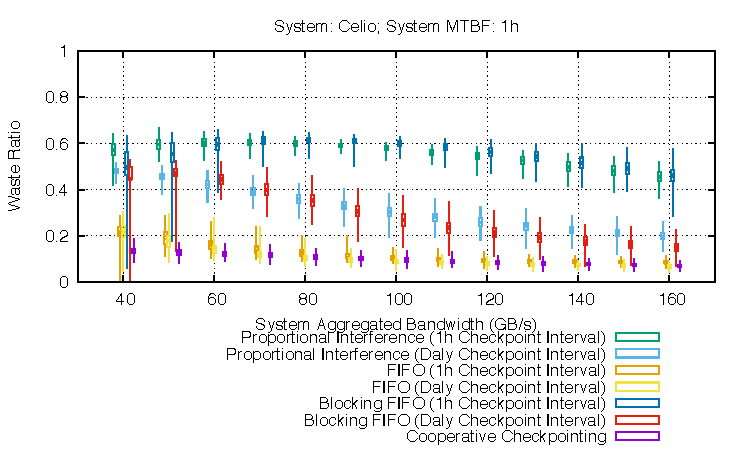
\includegraphics[width=\linewidth]{sim/figures/synthetic-01hMTBF-waste-celio.pdf}
  \end{center}
  \caption{Waste ratio as a function of the system bandwidth for the
    seven I/O and Checkpointing scheduling strategies, and the Cielo
    workload \label{fig:cielo-1hmtbf}}
\end{figure}

First, we explore the performance of each approach under heavy risks
of failures. Figure~\ref{fig:cielo-1hmtbf} represents the waste ratio
on Cielo, assuming the MTBF of the system was 1h. We vary the
filesystem bandwidth from 40 GB/s to 160GB/s in order to evaluate the
impact of this parameter. We observe 3 classes of behavior: \propfixed
and \bfifofixed exhibit a waste ratio that decrease as the bandwidth
increases, but remains above 40\% even with a high available
bandwidth; \fifodaly, \fifofixed, and \cooperative quickly decrese at
only 20\% of waste or less, and reach the theoretical model
performance; and \propdaly and \bfifodaly start at the same level of
efficiency as \propfixed and \bfifofixed, and reach the 20\% of waste
as the bandwidth increases.

This figure shows that with a high frequency of failures, providing
each application with the appropriate checkpoint interval is central
to relieve the filesystem from unecessary (or even detrimental)
checkpoints, but this is not the sole criteria that should be taken
into account. The two strategies that remain with a high waste despite
a high bandwidth rely on a fixed 1h interval. As the figure
illustrates, simply relying on the Daly checkpointing period is not
sufficient to reach the best performance under constrained bandwidth:
at 60GB/s for the filesystem, \propdaly and \bfifodaly experience
twice the waste of the other strategies relying on the same value for
the checkpointing period. All strategies that decouple the execution
of the application from the filesystem availability (\fifodaly,
\fifofixed, \cooperative) exhibit much better performance despite low
bandwidth.

Notably, \cooperative remains the most efficient technique under all
conditions, and reaches the theoretical performance given by
Equation~\eqref{eq.totalwaste} in the case of a stead state
analysis. This illustrates the efficiency of the proposed heuristic
(Equations~\eqref{eq.heuristicpart1} and~\eqref{eq.heuristicpart2}) to
schedule checkpoints and I/O in a way that avoids interferences,
allowing the system to behave as if no interference was experienced,
in most cases. The high variation shows that a minority of the runs
experienced a significantly higher waste.

\begin{figure}
  \begin{center}
    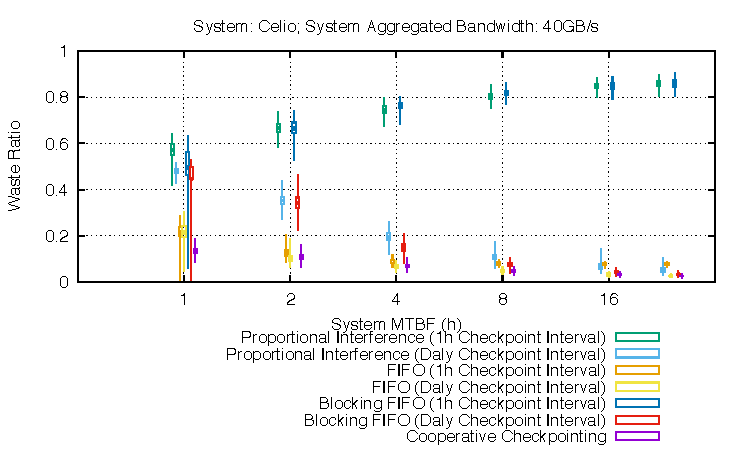
\includegraphics[width=\linewidth]{sim/figures/synthetic-040gbs-waste-celio.pdf}
  \end{center}
  \caption{Waste ratio as a function of the system MTBF for the
    seven I/O and Checkpointing scheduling strategies, and the Cielo
    workload \label{fig:cielo-40gbs}}
\end{figure}

Second, we explore the performance of each approach under low
bandwidth (and thus high risk of
interference). Figure~\ref{fig:cielo-40gbs} represents the waste ratio
on Cielo, assuming the aggregated filesystem bandwidth of the system
was 40GB/s. We vary the system MTBF from 1h (2 years of node MTBF) to
24h (48 years of node MTBF) in order to evaluate the impact of this
parameter. Similarly to Figure~\ref{fig:cielo-1hmtbf}, we observe 3
classes of behavior: \propfixed and \bfifofixed exhibit a waste ratio
that remains constant around 80\% for all values of the MTBF. These
appraoch are critically dependent on the filesystem bandwidth, and a
lower frequency of failures does not significantly improve their
performance. The I/O subsystem is saturated, and the applications
spends most of their time waiting for it. \fifodaly, \fifofixed, and
\cooperative quickly fall at only 20\% of waste or less, and reach
the theoretical model performance; and \propdaly and \bfifodaly start
at the same level of efficiency as \propfixed and \bfifofixed, and
reach the 20\% of waste as the bandwidth increases.

For all the strategies that integrate the Daly checkpointing period
optimization, increasing the MTBF reduces the amount of I/O required
and thus enables to manage a constrained bandwidth easily. All
strategies that schedule the bandwidth are succesful at increasing the
efficiency to values very close to the theoretical model. More
suprisingly, the simple FIFO scheduling of checkpoints with fixed
chekpoint interval (\bfifofixed) is capable of reaching a performance
comparable to the one of the strategies that reduce the number of
checkpoints. This is due to the significant reduction in interference
due to the reduction of number of restarts with an MTBF of 8h. As soon
as the number of restarting applications decreases, the filesystem
sollicitation decreases sufficiently to avoid long delays in non blocking
approaches, as is illustrated by the performance of \fifofixed at 2h
of MTBF.

\subsection{Prospective Systems}

% !TEX root =  ipdps18.tex

\section{Results}\label{sec:results}
% Primary: Thomas & all

\subsection{LANL APEX Simulation Workflows on Cielo}

We consider the workload from LANL found in the APEX Workflows
report~\cite{apex2016} that consists of four applications classes: EAP, LAP,
Silverton and VPIC. The main characteristics of these classes are reported in
Table~\ref{table:lanl}. We simulate the behavior of these applications on the
Cielo Platform. Cielo was a 1.37 Petaflops capability system operated from 2010
to 2016 at the Los Alamos National Laboratory.  It consisted of 143,104 cores,
286 TB of main memory, and a parallel filesystem with a theoretical maximum
capacity of 160GB/s.  Cielo was chosen for this initial analysis due to the
availability of the aforementioned workflows report, something not available for
other platforms. In later sections, we consider similar workloads on a more
modern platform.

\begin{table}
\begin{tabular}{|l|c|c|c|c|}
\hline
 Workflow & EAP & LAP & Silverton & VPIC \\\hline
Workload percentage & 66 & 5.5 & 16.5 & 12 \\\hline
Work time (h) & 262.4 & 64 & 128 & 157.2 \\\hline
Number of cores & 16384 & 4096 & 32768 & 30000 \\\hline
Initial Input (\% of memory) &  3 & 5 & 70 & 10 \\\hline
Final Output (\% of memory) & 105 & 220 & 43 & 270 \\\hline
Checkpoint Size (\% of memory) & 160 & 185 & 350 & 85 \\\hline
\end{tabular}
\caption{LANL Workflow Workload from the APEX Workflows report.\label{table:lanl}}
\end{table}

The baseline in this comparison comprises a set of simulations with no faults,
checkpoints, nor I/O interference. For these simulations, we selected a 60-day
execution segment, and computed the resources used by the jobs during this
period, \ie the total time each node spent on (non-CR) I/O and computation in a
failure-free environment.

For the I/O scheduling techniques presented in Section~\ref{sec:algorithms}, we
compute the resource waste as the total time nodes spend not progressing jobs.
In the figures presented, we represent the performance of each strategy by
computing the waste ratio, \ie the resource waste over a segment of 60 days
divided by the application resource usage over that same segment for the
baseline simulation. Each simulation is conducted over 1,000 times; the
candlestick extremes represent the first and last decile of the measures, while
the boxes represent the first and last quartile, and the center the mean value.

\begin{figure}
  \begin{center}
    \resizebox{1.05\linewidth}{!}{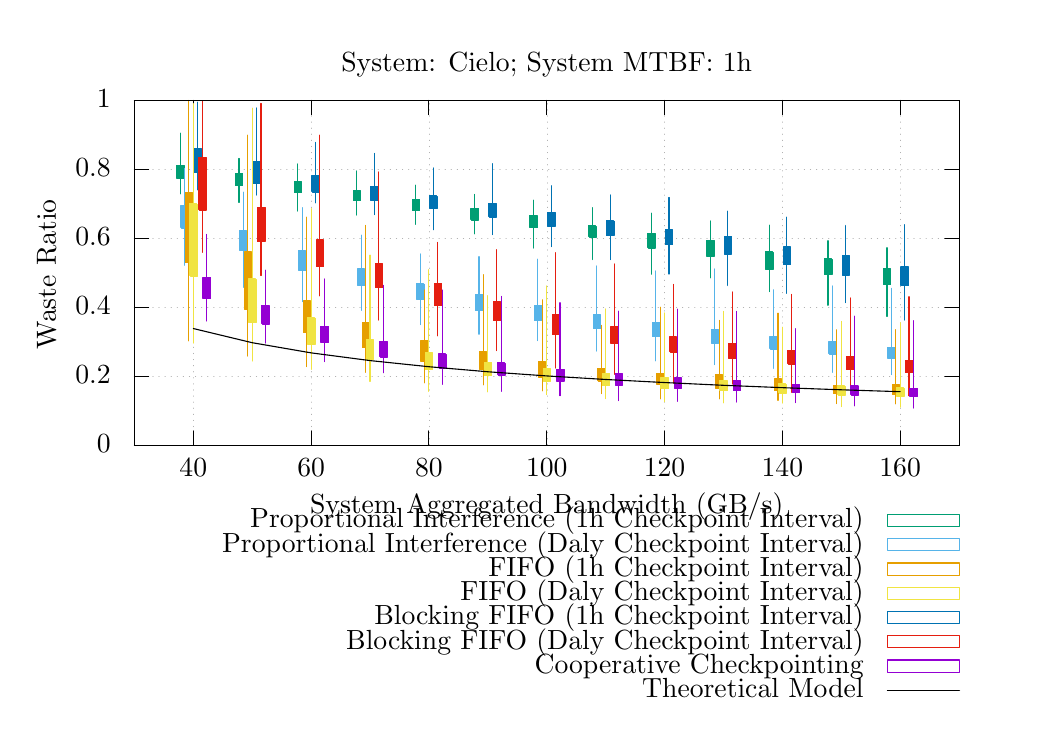
\begin{tikzpicture}[gnuplot]
%% generated with GNUPLOT 5.0p6 (Lua 5.3; terminal rev. 99, script rev. 100)
%% Wed Oct 18 12:28:52 2017
\path (0.000,0.000) rectangle (12.500,8.750);
\gpcolor{color=gp lt color axes}
\gpsetlinetype{gp lt axes}
\gpsetdashtype{gp dt axes}
\gpsetlinewidth{0.50}
\draw[gp path] (1.320,3.449)--(11.793,3.449);
\gpcolor{color=gp lt color border}
\gpsetlinetype{gp lt border}
\gpsetdashtype{gp dt solid}
\gpsetlinewidth{1.00}
\draw[gp path] (1.320,3.449)--(1.500,3.449);
\draw[gp path] (11.793,3.449)--(11.613,3.449);
\node[gp node right] at (1.136,3.449) {$0$};
\gpcolor{color=gp lt color axes}
\gpsetlinetype{gp lt axes}
\gpsetdashtype{gp dt axes}
\gpsetlinewidth{0.50}
\draw[gp path] (1.320,4.324)--(11.793,4.324);
\gpcolor{color=gp lt color border}
\gpsetlinetype{gp lt border}
\gpsetdashtype{gp dt solid}
\gpsetlinewidth{1.00}
\draw[gp path] (1.320,4.324)--(1.500,4.324);
\draw[gp path] (11.793,4.324)--(11.613,4.324);
\node[gp node right] at (1.136,4.324) {$0.2$};
\gpcolor{color=gp lt color axes}
\gpsetlinetype{gp lt axes}
\gpsetdashtype{gp dt axes}
\gpsetlinewidth{0.50}
\draw[gp path] (1.320,5.199)--(11.793,5.199);
\gpcolor{color=gp lt color border}
\gpsetlinetype{gp lt border}
\gpsetdashtype{gp dt solid}
\gpsetlinewidth{1.00}
\draw[gp path] (1.320,5.199)--(1.500,5.199);
\draw[gp path] (11.793,5.199)--(11.613,5.199);
\node[gp node right] at (1.136,5.199) {$0.4$};
\gpcolor{color=gp lt color axes}
\gpsetlinetype{gp lt axes}
\gpsetdashtype{gp dt axes}
\gpsetlinewidth{0.50}
\draw[gp path] (1.320,6.075)--(11.793,6.075);
\gpcolor{color=gp lt color border}
\gpsetlinetype{gp lt border}
\gpsetdashtype{gp dt solid}
\gpsetlinewidth{1.00}
\draw[gp path] (1.320,6.075)--(1.500,6.075);
\draw[gp path] (11.793,6.075)--(11.613,6.075);
\node[gp node right] at (1.136,6.075) {$0.6$};
\gpcolor{color=gp lt color axes}
\gpsetlinetype{gp lt axes}
\gpsetdashtype{gp dt axes}
\gpsetlinewidth{0.50}
\draw[gp path] (1.320,6.950)--(11.793,6.950);
\gpcolor{color=gp lt color border}
\gpsetlinetype{gp lt border}
\gpsetdashtype{gp dt solid}
\gpsetlinewidth{1.00}
\draw[gp path] (1.320,6.950)--(1.500,6.950);
\draw[gp path] (11.793,6.950)--(11.613,6.950);
\node[gp node right] at (1.136,6.950) {$0.8$};
\gpcolor{color=gp lt color axes}
\gpsetlinetype{gp lt axes}
\gpsetdashtype{gp dt axes}
\gpsetlinewidth{0.50}
\draw[gp path] (1.320,7.825)--(11.793,7.825);
\gpcolor{color=gp lt color border}
\gpsetlinetype{gp lt border}
\gpsetdashtype{gp dt solid}
\gpsetlinewidth{1.00}
\draw[gp path] (1.320,7.825)--(1.500,7.825);
\draw[gp path] (11.793,7.825)--(11.613,7.825);
\node[gp node right] at (1.136,7.825) {$1$};
\gpcolor{color=gp lt color axes}
\gpsetlinetype{gp lt axes}
\gpsetdashtype{gp dt axes}
\gpsetlinewidth{0.50}
\draw[gp path] (2.068,3.449)--(2.068,7.825);
\gpcolor{color=gp lt color border}
\gpsetlinetype{gp lt border}
\gpsetdashtype{gp dt solid}
\gpsetlinewidth{1.00}
\draw[gp path] (2.068,3.449)--(2.068,3.629);
\draw[gp path] (2.068,7.825)--(2.068,7.645);
\node[gp node center] at (2.068,3.141) {$40$};
\gpcolor{color=gp lt color axes}
\gpsetlinetype{gp lt axes}
\gpsetdashtype{gp dt axes}
\gpsetlinewidth{0.50}
\draw[gp path] (3.564,3.449)--(3.564,7.825);
\gpcolor{color=gp lt color border}
\gpsetlinetype{gp lt border}
\gpsetdashtype{gp dt solid}
\gpsetlinewidth{1.00}
\draw[gp path] (3.564,3.449)--(3.564,3.629);
\draw[gp path] (3.564,7.825)--(3.564,7.645);
\node[gp node center] at (3.564,3.141) {$60$};
\gpcolor{color=gp lt color axes}
\gpsetlinetype{gp lt axes}
\gpsetdashtype{gp dt axes}
\gpsetlinewidth{0.50}
\draw[gp path] (5.060,3.449)--(5.060,7.825);
\gpcolor{color=gp lt color border}
\gpsetlinetype{gp lt border}
\gpsetdashtype{gp dt solid}
\gpsetlinewidth{1.00}
\draw[gp path] (5.060,3.449)--(5.060,3.629);
\draw[gp path] (5.060,7.825)--(5.060,7.645);
\node[gp node center] at (5.060,3.141) {$80$};
\gpcolor{color=gp lt color axes}
\gpsetlinetype{gp lt axes}
\gpsetdashtype{gp dt axes}
\gpsetlinewidth{0.50}
\draw[gp path] (6.557,3.449)--(6.557,7.825);
\gpcolor{color=gp lt color border}
\gpsetlinetype{gp lt border}
\gpsetdashtype{gp dt solid}
\gpsetlinewidth{1.00}
\draw[gp path] (6.557,3.449)--(6.557,3.629);
\draw[gp path] (6.557,7.825)--(6.557,7.645);
\node[gp node center] at (6.557,3.141) {$100$};
\gpcolor{color=gp lt color axes}
\gpsetlinetype{gp lt axes}
\gpsetdashtype{gp dt axes}
\gpsetlinewidth{0.50}
\draw[gp path] (8.053,3.449)--(8.053,7.825);
\gpcolor{color=gp lt color border}
\gpsetlinetype{gp lt border}
\gpsetdashtype{gp dt solid}
\gpsetlinewidth{1.00}
\draw[gp path] (8.053,3.449)--(8.053,3.629);
\draw[gp path] (8.053,7.825)--(8.053,7.645);
\node[gp node center] at (8.053,3.141) {$120$};
\gpcolor{color=gp lt color axes}
\gpsetlinetype{gp lt axes}
\gpsetdashtype{gp dt axes}
\gpsetlinewidth{0.50}
\draw[gp path] (9.549,3.449)--(9.549,7.825);
\gpcolor{color=gp lt color border}
\gpsetlinetype{gp lt border}
\gpsetdashtype{gp dt solid}
\gpsetlinewidth{1.00}
\draw[gp path] (9.549,3.449)--(9.549,3.629);
\draw[gp path] (9.549,7.825)--(9.549,7.645);
\node[gp node center] at (9.549,3.141) {$140$};
\gpcolor{color=gp lt color axes}
\gpsetlinetype{gp lt axes}
\gpsetdashtype{gp dt axes}
\gpsetlinewidth{0.50}
\draw[gp path] (11.045,3.449)--(11.045,7.825);
\gpcolor{color=gp lt color border}
\gpsetlinetype{gp lt border}
\gpsetdashtype{gp dt solid}
\gpsetlinewidth{1.00}
\draw[gp path] (11.045,3.449)--(11.045,3.629);
\draw[gp path] (11.045,7.825)--(11.045,7.645);
\node[gp node center] at (11.045,3.141) {$160$};
\draw[gp path] (1.320,7.825)--(1.320,3.449)--(11.793,3.449)--(11.793,7.825)--cycle;
\node[gp node center,rotate=-270] at (0.246,5.637) {Waste Ratio};
\node[gp node center] at (6.556,2.679) {System Aggregated Bandwidth (GB/s)};
\node[gp node center] at (6.556,8.287) {System: Cielo; System MTBF: 1h};
\node[gp node right] at (10.698,2.490) {Proportional Interference (1h Checkpoint Interval)};
\gpcolor{rgb color={0.000,0.620,0.451}}
\draw[gp path] (10.882,2.413)--(11.798,2.413)--(11.798,2.567)--(10.882,2.567)--cycle;
\gpfill{rgb color={0.000,0.620,0.451}} (1.855,6.846)--(1.945,6.846)--(1.945,7.004)--(1.855,7.004)--cycle;
\draw[gp path] (1.900,6.639)--(1.900,6.846);
\draw[gp path] (1.900,7.004)--(1.900,7.409);
\draw[gp path] (1.855,7.004)--(1.945,7.004)--(1.945,6.846)--(1.855,6.846)--cycle;
\gpfill{rgb color={0.000,0.620,0.451}} (2.603,6.745)--(2.693,6.745)--(2.693,6.898)--(2.603,6.898)--cycle;
\draw[gp path] (2.648,6.531)--(2.648,6.745);
\draw[gp path] (2.648,6.898)--(2.648,7.089);
\draw[gp path] (2.603,6.898)--(2.693,6.898)--(2.693,6.745)--(2.603,6.745)--cycle;
\gpfill{rgb color={0.000,0.620,0.451}} (3.351,6.658)--(3.441,6.658)--(3.441,6.795)--(3.351,6.795)--cycle;
\draw[gp path] (3.396,6.420)--(3.396,6.658);
\draw[gp path] (3.396,6.795)--(3.396,7.021);
\draw[gp path] (3.351,6.795)--(3.441,6.795)--(3.441,6.658)--(3.351,6.658)--cycle;
\gpfill{rgb color={0.000,0.620,0.451}} (4.099,6.559)--(4.189,6.559)--(4.189,6.680)--(4.099,6.680)--cycle;
\draw[gp path] (4.144,6.369)--(4.144,6.559);
\draw[gp path] (4.144,6.680)--(4.144,6.931);
\draw[gp path] (4.099,6.680)--(4.189,6.680)--(4.189,6.559)--(4.099,6.559)--cycle;
\gpfill{rgb color={0.000,0.620,0.451}} (4.847,6.432)--(4.937,6.432)--(4.937,6.570)--(4.847,6.570)--cycle;
\draw[gp path] (4.892,6.253)--(4.892,6.432);
\draw[gp path] (4.892,6.570)--(4.892,6.749);
\draw[gp path] (4.847,6.570)--(4.937,6.570)--(4.937,6.432)--(4.847,6.432)--cycle;
\gpfill{rgb color={0.000,0.620,0.451}} (5.595,6.313)--(5.685,6.313)--(5.685,6.454)--(5.595,6.454)--cycle;
\draw[gp path] (5.640,6.132)--(5.640,6.313);
\draw[gp path] (5.640,6.454)--(5.640,6.633);
\draw[gp path] (5.595,6.454)--(5.685,6.454)--(5.685,6.313)--(5.595,6.313)--cycle;
\gpfill{rgb color={0.000,0.620,0.451}} (6.343,6.215)--(6.433,6.215)--(6.433,6.360)--(6.343,6.360)--cycle;
\draw[gp path] (6.388,5.952)--(6.388,6.215);
\draw[gp path] (6.388,6.360)--(6.388,6.560);
\draw[gp path] (6.343,6.360)--(6.433,6.360)--(6.433,6.215)--(6.343,6.215)--cycle;
\gpfill{rgb color={0.000,0.620,0.451}} (7.091,6.096)--(7.181,6.096)--(7.181,6.232)--(7.091,6.232)--cycle;
\draw[gp path] (7.136,5.806)--(7.136,6.096);
\draw[gp path] (7.136,6.232)--(7.136,6.463);
\draw[gp path] (7.091,6.232)--(7.181,6.232)--(7.181,6.096)--(7.091,6.096)--cycle;
\gpfill{rgb color={0.000,0.620,0.451}} (7.839,5.957)--(7.929,5.957)--(7.929,6.140)--(7.839,6.140)--cycle;
\draw[gp path] (7.884,5.619)--(7.884,5.957);
\draw[gp path] (7.884,6.140)--(7.884,6.395);
\draw[gp path] (7.839,6.140)--(7.929,6.140)--(7.929,5.957)--(7.839,5.957)--cycle;
\gpfill{rgb color={0.000,0.620,0.451}} (8.587,5.850)--(8.677,5.850)--(8.677,6.052)--(8.587,6.052)--cycle;
\draw[gp path] (8.632,5.572)--(8.632,5.850);
\draw[gp path] (8.632,6.052)--(8.632,6.296);
\draw[gp path] (8.587,6.052)--(8.677,6.052)--(8.677,5.850)--(8.587,5.850)--cycle;
\gpfill{rgb color={0.000,0.620,0.451}} (9.335,5.687)--(9.425,5.687)--(9.425,5.905)--(9.335,5.905)--cycle;
\draw[gp path] (9.380,5.397)--(9.380,5.687);
\draw[gp path] (9.380,5.905)--(9.380,6.243);
\draw[gp path] (9.335,5.905)--(9.425,5.905)--(9.425,5.687)--(9.335,5.687)--cycle;
\gpfill{rgb color={0.000,0.620,0.451}} (10.084,5.621)--(10.174,5.621)--(10.174,5.813)--(10.084,5.813)--cycle;
\draw[gp path] (10.129,5.225)--(10.129,5.621);
\draw[gp path] (10.129,5.813)--(10.129,6.044);
\draw[gp path] (10.084,5.813)--(10.174,5.813)--(10.174,5.621)--(10.084,5.621)--cycle;
\gpfill{rgb color={0.000,0.620,0.451}} (10.832,5.495)--(10.922,5.495)--(10.922,5.690)--(10.832,5.690)--cycle;
\draw[gp path] (10.877,5.083)--(10.877,5.495);
\draw[gp path] (10.877,5.690)--(10.877,5.956);
\draw[gp path] (10.832,5.690)--(10.922,5.690)--(10.922,5.495)--(10.832,5.495)--cycle;
\gpsetpointsize{0.80}
\gppoint{gp mark 2}{(1.900,6.931)}
\gppoint{gp mark 2}{(2.648,6.824)}
\gppoint{gp mark 2}{(3.396,6.729)}
\gppoint{gp mark 2}{(4.144,6.622)}
\gppoint{gp mark 2}{(4.892,6.500)}
\gppoint{gp mark 2}{(5.640,6.383)}
\gppoint{gp mark 2}{(6.388,6.284)}
\gppoint{gp mark 2}{(7.136,6.160)}
\gppoint{gp mark 2}{(7.884,6.047)}
\gppoint{gp mark 2}{(8.632,5.947)}
\gppoint{gp mark 2}{(9.380,5.798)}
\gppoint{gp mark 2}{(10.129,5.712)}
\gppoint{gp mark 2}{(10.877,5.589)}
\gpcolor{color=gp lt color border}
\node[gp node right] at (10.698,2.182) {Proportional Interference (Daly Checkpoint Interval)};
\gpcolor{rgb color={0.337,0.706,0.914}}
\draw[gp path] (10.882,2.105)--(11.798,2.105)--(11.798,2.259)--(10.882,2.259)--cycle;
\gpfill{rgb color={0.337,0.706,0.914}} (1.911,6.207)--(2.001,6.207)--(2.001,6.491)--(1.911,6.491)--cycle;
\draw[gp path] (1.956,5.733)--(1.956,6.207);
\draw[gp path] (1.956,6.491)--(1.956,6.962);
\draw[gp path] (1.911,6.491)--(2.001,6.491)--(2.001,6.207)--(1.911,6.207)--cycle;
\gpfill{rgb color={0.337,0.706,0.914}} (2.659,5.920)--(2.749,5.920)--(2.749,6.172)--(2.659,6.172)--cycle;
\draw[gp path] (2.704,5.453)--(2.704,5.920);
\draw[gp path] (2.704,6.172)--(2.704,6.660);
\draw[gp path] (2.659,6.172)--(2.749,6.172)--(2.749,5.920)--(2.659,5.920)--cycle;
\gpfill{rgb color={0.337,0.706,0.914}} (3.407,5.670)--(3.497,5.670)--(3.497,5.915)--(3.407,5.915)--cycle;
\draw[gp path] (3.452,5.272)--(3.452,5.670);
\draw[gp path] (3.452,5.915)--(3.452,6.464);
\draw[gp path] (3.407,5.915)--(3.497,5.915)--(3.497,5.670)--(3.407,5.670)--cycle;
\gpfill{rgb color={0.337,0.706,0.914}} (4.155,5.480)--(4.245,5.480)--(4.245,5.685)--(4.155,5.685)--cycle;
\draw[gp path] (4.200,5.160)--(4.200,5.480);
\draw[gp path] (4.200,5.685)--(4.200,6.115);
\draw[gp path] (4.155,5.685)--(4.245,5.685)--(4.245,5.480)--(4.155,5.480)--cycle;
\gpfill{rgb color={0.337,0.706,0.914}} (4.903,5.306)--(4.993,5.306)--(4.993,5.500)--(4.903,5.500)--cycle;
\draw[gp path] (4.948,4.980)--(4.948,5.306);
\draw[gp path] (4.948,5.500)--(4.948,5.876);
\draw[gp path] (4.903,5.500)--(4.993,5.500)--(4.993,5.306)--(4.903,5.306)--cycle;
\gpfill{rgb color={0.337,0.706,0.914}} (5.651,5.165)--(5.741,5.165)--(5.741,5.361)--(5.651,5.361)--cycle;
\draw[gp path] (5.696,4.857)--(5.696,5.165);
\draw[gp path] (5.696,5.361)--(5.696,5.842);
\draw[gp path] (5.651,5.361)--(5.741,5.361)--(5.741,5.165)--(5.651,5.165)--cycle;
\gpfill{rgb color={0.337,0.706,0.914}} (6.399,5.038)--(6.489,5.038)--(6.489,5.224)--(6.399,5.224)--cycle;
\draw[gp path] (6.444,4.777)--(6.444,5.038);
\draw[gp path] (6.444,5.224)--(6.444,5.809);
\draw[gp path] (6.399,5.224)--(6.489,5.224)--(6.489,5.038)--(6.399,5.038)--cycle;
\gpfill{rgb color={0.337,0.706,0.914}} (7.147,4.930)--(7.237,4.930)--(7.237,5.103)--(7.147,5.103)--cycle;
\draw[gp path] (7.192,4.642)--(7.192,4.930);
\draw[gp path] (7.192,5.103)--(7.192,5.723);
\draw[gp path] (7.147,5.103)--(7.237,5.103)--(7.237,4.930)--(7.147,4.930)--cycle;
\gpfill{rgb color={0.337,0.706,0.914}} (7.895,4.832)--(7.985,4.832)--(7.985,5.006)--(7.895,5.006)--cycle;
\draw[gp path] (7.940,4.520)--(7.940,4.832);
\draw[gp path] (7.940,5.006)--(7.940,5.660);
\draw[gp path] (7.895,5.006)--(7.985,5.006)--(7.985,4.832)--(7.895,4.832)--cycle;
\gpfill{rgb color={0.337,0.706,0.914}} (8.644,4.748)--(8.734,4.748)--(8.734,4.913)--(8.644,4.913)--cycle;
\draw[gp path] (8.689,4.472)--(8.689,4.748);
\draw[gp path] (8.689,4.913)--(8.689,5.685);
\draw[gp path] (8.644,4.913)--(8.734,4.913)--(8.734,4.748)--(8.644,4.748)--cycle;
\gpfill{rgb color={0.337,0.706,0.914}} (9.392,4.670)--(9.482,4.670)--(9.482,4.828)--(9.392,4.828)--cycle;
\draw[gp path] (9.437,4.422)--(9.437,4.670);
\draw[gp path] (9.437,4.828)--(9.437,5.421);
\draw[gp path] (9.392,4.828)--(9.482,4.828)--(9.482,4.670)--(9.392,4.670)--cycle;
\gpfill{rgb color={0.337,0.706,0.914}} (10.140,4.610)--(10.230,4.610)--(10.230,4.758)--(10.140,4.758)--cycle;
\draw[gp path] (10.185,4.372)--(10.185,4.610);
\draw[gp path] (10.185,4.758)--(10.185,5.470);
\draw[gp path] (10.140,4.758)--(10.230,4.758)--(10.230,4.610)--(10.140,4.610)--cycle;
\gpfill{rgb color={0.337,0.706,0.914}} (10.888,4.555)--(10.978,4.555)--(10.978,4.693)--(10.888,4.693)--cycle;
\draw[gp path] (10.933,4.345)--(10.933,4.555);
\draw[gp path] (10.933,4.693)--(10.933,5.440);
\draw[gp path] (10.888,4.693)--(10.978,4.693)--(10.978,4.555)--(10.888,4.555)--cycle;
\gppoint{gp mark 3}{(1.956,6.355)}
\gppoint{gp mark 3}{(2.704,6.044)}
\gppoint{gp mark 3}{(3.452,5.792)}
\gppoint{gp mark 3}{(4.200,5.580)}
\gppoint{gp mark 3}{(4.948,5.406)}
\gppoint{gp mark 3}{(5.696,5.265)}
\gppoint{gp mark 3}{(6.444,5.137)}
\gppoint{gp mark 3}{(7.192,5.025)}
\gppoint{gp mark 3}{(7.940,4.929)}
\gppoint{gp mark 3}{(8.689,4.848)}
\gppoint{gp mark 3}{(9.437,4.764)}
\gppoint{gp mark 3}{(10.185,4.701)}
\gppoint{gp mark 3}{(10.933,4.644)}
\gpcolor{color=gp lt color border}
\node[gp node right] at (10.698,1.874) {FIFO (1h Checkpoint Interval)};
\gpcolor{rgb color={0.902,0.624,0.000}}
\draw[gp path] (10.882,1.797)--(11.798,1.797)--(11.798,1.951)--(10.882,1.951)--cycle;
\gpfill{rgb color={0.902,0.624,0.000}} (1.967,5.767)--(2.057,5.767)--(2.057,6.655)--(1.967,6.655)--cycle;
\draw[gp path] (2.012,4.772)--(2.012,5.767);
\draw[gp path] (2.012,6.655)--(2.012,7.825);
\draw[gp path] (1.967,6.655)--(2.057,6.655)--(2.057,5.767)--(1.967,5.767)--cycle;
\gpfill{rgb color={0.902,0.624,0.000}} (2.715,5.179)--(2.805,5.179)--(2.805,5.901)--(2.715,5.901)--cycle;
\draw[gp path] (2.760,4.580)--(2.760,5.179);
\draw[gp path] (2.760,5.901)--(2.760,7.386);
\draw[gp path] (2.715,5.901)--(2.805,5.901)--(2.805,5.179)--(2.715,5.179)--cycle;
\gpfill{rgb color={0.902,0.624,0.000}} (3.463,4.884)--(3.553,4.884)--(3.553,5.279)--(3.463,5.279)--cycle;
\draw[gp path] (3.508,4.446)--(3.508,4.884);
\draw[gp path] (3.508,5.279)--(3.508,6.344);
\draw[gp path] (3.463,5.279)--(3.553,5.279)--(3.553,4.884)--(3.463,4.884)--cycle;
\gpfill{rgb color={0.902,0.624,0.000}} (4.211,4.695)--(4.301,4.695)--(4.301,5.008)--(4.211,5.008)--cycle;
\draw[gp path] (4.256,4.373)--(4.256,4.695);
\draw[gp path] (4.256,5.008)--(4.256,6.238);
\draw[gp path] (4.211,5.008)--(4.301,5.008)--(4.301,4.695)--(4.211,4.695)--cycle;
\gpfill{rgb color={0.902,0.624,0.000}} (4.959,4.513)--(5.049,4.513)--(5.049,4.772)--(4.959,4.772)--cycle;
\draw[gp path] (5.004,4.240)--(5.004,4.513);
\draw[gp path] (5.004,4.772)--(5.004,5.419);
\draw[gp path] (4.959,4.772)--(5.049,4.772)--(5.049,4.513)--(4.959,4.513)--cycle;
\gpfill{rgb color={0.902,0.624,0.000}} (5.707,4.409)--(5.797,4.409)--(5.797,4.632)--(5.707,4.632)--cycle;
\draw[gp path] (5.752,4.214)--(5.752,4.409);
\draw[gp path] (5.752,4.632)--(5.752,5.613);
\draw[gp path] (5.707,4.632)--(5.797,4.632)--(5.797,4.409)--(5.707,4.409)--cycle;
\gpfill{rgb color={0.902,0.624,0.000}} (6.455,4.312)--(6.545,4.312)--(6.545,4.505)--(6.455,4.505)--cycle;
\draw[gp path] (6.500,4.139)--(6.500,4.312);
\draw[gp path] (6.500,4.505)--(6.500,5.294);
\draw[gp path] (6.455,4.505)--(6.545,4.505)--(6.545,4.312)--(6.455,4.312)--cycle;
\gpfill{rgb color={0.902,0.624,0.000}} (7.203,4.268)--(7.293,4.268)--(7.293,4.427)--(7.203,4.427)--cycle;
\draw[gp path] (7.248,4.103)--(7.248,4.268);
\draw[gp path] (7.248,4.427)--(7.248,4.968);
\draw[gp path] (7.203,4.427)--(7.293,4.427)--(7.293,4.268)--(7.203,4.268)--cycle;
\gpfill{rgb color={0.902,0.624,0.000}} (7.952,4.225)--(8.042,4.225)--(8.042,4.362)--(7.952,4.362)--cycle;
\draw[gp path] (7.997,4.035)--(7.997,4.225);
\draw[gp path] (7.997,4.362)--(7.997,5.199);
\draw[gp path] (7.952,4.362)--(8.042,4.362)--(8.042,4.225)--(7.952,4.225)--cycle;
\gpfill{rgb color={0.902,0.624,0.000}} (8.700,4.177)--(8.790,4.177)--(8.790,4.343)--(8.700,4.343)--cycle;
\draw[gp path] (8.745,4.035)--(8.745,4.177);
\draw[gp path] (8.745,4.343)--(8.745,5.031);
\draw[gp path] (8.700,4.343)--(8.790,4.343)--(8.790,4.177)--(8.700,4.177)--cycle;
\gpfill{rgb color={0.902,0.624,0.000}} (9.448,4.149)--(9.538,4.149)--(9.538,4.288)--(9.448,4.288)--cycle;
\draw[gp path] (9.493,4.017)--(9.493,4.149);
\draw[gp path] (9.493,4.288)--(9.493,5.124);
\draw[gp path] (9.448,4.288)--(9.538,4.288)--(9.538,4.149)--(9.448,4.149)--cycle;
\gpfill{rgb color={0.902,0.624,0.000}} (10.196,4.109)--(10.286,4.109)--(10.286,4.211)--(10.196,4.211)--cycle;
\draw[gp path] (10.241,3.977)--(10.241,4.109);
\draw[gp path] (10.241,4.211)--(10.241,4.913);
\draw[gp path] (10.196,4.211)--(10.286,4.211)--(10.286,4.109)--(10.196,4.109)--cycle;
\gpfill{rgb color={0.902,0.624,0.000}} (10.944,4.094)--(11.034,4.094)--(11.034,4.215)--(10.944,4.215)--cycle;
\draw[gp path] (10.989,3.974)--(10.989,4.094);
\draw[gp path] (10.989,4.215)--(10.989,4.916);
\draw[gp path] (10.944,4.215)--(11.034,4.215)--(11.034,4.094)--(10.944,4.094)--cycle;
\gppoint{gp mark 4}{(2.012,6.245)}
\gppoint{gp mark 4}{(2.760,5.585)}
\gppoint{gp mark 4}{(3.508,5.106)}
\gppoint{gp mark 4}{(4.256,4.873)}
\gppoint{gp mark 4}{(5.004,4.658)}
\gppoint{gp mark 4}{(5.752,4.542)}
\gppoint{gp mark 4}{(6.500,4.435)}
\gppoint{gp mark 4}{(7.248,4.373)}
\gppoint{gp mark 4}{(7.997,4.327)}
\gppoint{gp mark 4}{(8.745,4.292)}
\gppoint{gp mark 4}{(9.493,4.247)}
\gppoint{gp mark 4}{(10.241,4.184)}
\gppoint{gp mark 4}{(10.989,4.195)}
\gpcolor{color=gp lt color border}
\node[gp node right] at (10.698,1.566) {FIFO (Daly Checkpoint Interval)};
\gpcolor{rgb color={0.941,0.894,0.259}}
\draw[gp path] (10.882,1.489)--(11.798,1.489)--(11.798,1.643)--(10.882,1.643)--cycle;
\gpfill{rgb color={0.941,0.894,0.259}} (2.023,5.597)--(2.113,5.597)--(2.113,6.515)--(2.023,6.515)--cycle;
\draw[gp path] (2.068,4.744)--(2.068,5.597);
\draw[gp path] (2.068,6.515)--(2.068,7.784);
\draw[gp path] (2.023,6.515)--(2.113,6.515)--(2.113,5.597)--(2.023,5.597)--cycle;
\gpfill{rgb color={0.941,0.894,0.259}} (2.771,5.011)--(2.861,5.011)--(2.861,5.558)--(2.771,5.558)--cycle;
\draw[gp path] (2.816,4.517)--(2.816,5.011);
\draw[gp path] (2.816,5.558)--(2.816,7.727);
\draw[gp path] (2.771,5.558)--(2.861,5.558)--(2.861,5.011)--(2.771,5.011)--cycle;
\gpfill{rgb color={0.941,0.894,0.259}} (3.519,4.728)--(3.609,4.728)--(3.609,5.067)--(3.519,5.067)--cycle;
\draw[gp path] (3.564,4.410)--(3.564,4.728);
\draw[gp path] (3.564,5.067)--(3.564,6.453);
\draw[gp path] (3.519,5.067)--(3.609,5.067)--(3.609,4.728)--(3.519,4.728)--cycle;
\gpfill{rgb color={0.941,0.894,0.259}} (4.267,4.544)--(4.357,4.544)--(4.357,4.785)--(4.267,4.785)--cycle;
\draw[gp path] (4.312,4.257)--(4.312,4.544);
\draw[gp path] (4.312,4.785)--(4.312,5.861);
\draw[gp path] (4.267,4.785)--(4.357,4.785)--(4.357,4.544)--(4.267,4.544)--cycle;
\gpfill{rgb color={0.941,0.894,0.259}} (5.015,4.412)--(5.105,4.412)--(5.105,4.622)--(5.015,4.622)--cycle;
\draw[gp path] (5.060,4.130)--(5.060,4.412);
\draw[gp path] (5.060,4.622)--(5.060,5.677);
\draw[gp path] (5.015,4.622)--(5.105,4.622)--(5.105,4.412)--(5.015,4.412)--cycle;
\gpfill{rgb color={0.941,0.894,0.259}} (5.763,4.337)--(5.853,4.337)--(5.853,4.502)--(5.763,4.502)--cycle;
\draw[gp path] (5.808,4.125)--(5.808,4.337);
\draw[gp path] (5.808,4.502)--(5.808,5.347);
\draw[gp path] (5.763,4.502)--(5.853,4.502)--(5.853,4.337)--(5.763,4.337)--cycle;
\gpfill{rgb color={0.941,0.894,0.259}} (6.512,4.265)--(6.602,4.265)--(6.602,4.419)--(6.512,4.419)--cycle;
\draw[gp path] (6.557,4.091)--(6.557,4.265);
\draw[gp path] (6.557,4.419)--(6.557,5.471);
\draw[gp path] (6.512,4.419)--(6.602,4.419)--(6.602,4.265)--(6.512,4.265)--cycle;
\gpfill{rgb color={0.941,0.894,0.259}} (7.260,4.210)--(7.350,4.210)--(7.350,4.358)--(7.260,4.358)--cycle;
\draw[gp path] (7.305,4.038)--(7.305,4.210);
\draw[gp path] (7.305,4.358)--(7.305,5.177);
\draw[gp path] (7.260,4.358)--(7.350,4.358)--(7.350,4.210)--(7.260,4.210)--cycle;
\gpfill{rgb color={0.941,0.894,0.259}} (8.008,4.173)--(8.098,4.173)--(8.098,4.302)--(8.008,4.302)--cycle;
\draw[gp path] (8.053,4.000)--(8.053,4.173);
\draw[gp path] (8.053,4.302)--(8.053,5.127);
\draw[gp path] (8.008,4.302)--(8.098,4.302)--(8.098,4.173)--(8.008,4.173)--cycle;
\gpfill{rgb color={0.941,0.894,0.259}} (8.756,4.142)--(8.846,4.142)--(8.846,4.268)--(8.756,4.268)--cycle;
\draw[gp path] (8.801,3.984)--(8.801,4.142);
\draw[gp path] (8.801,4.268)--(8.801,5.146);
\draw[gp path] (8.756,4.268)--(8.846,4.268)--(8.846,4.142)--(8.756,4.142)--cycle;
\gpfill{rgb color={0.941,0.894,0.259}} (9.504,4.115)--(9.594,4.115)--(9.594,4.226)--(9.504,4.226)--cycle;
\draw[gp path] (9.549,3.981)--(9.549,4.115);
\draw[gp path] (9.549,4.226)--(9.549,4.945);
\draw[gp path] (9.504,4.226)--(9.594,4.226)--(9.594,4.115)--(9.504,4.115)--cycle;
\gpfill{rgb color={0.941,0.894,0.259}} (10.252,4.089)--(10.342,4.089)--(10.342,4.199)--(10.252,4.199)--cycle;
\draw[gp path] (10.297,3.938)--(10.297,4.089);
\draw[gp path] (10.297,4.199)--(10.297,5.020);
\draw[gp path] (10.252,4.199)--(10.342,4.199)--(10.342,4.089)--(10.252,4.089)--cycle;
\gpfill{rgb color={0.941,0.894,0.259}} (11.000,4.072)--(11.090,4.072)--(11.090,4.175)--(11.000,4.175)--cycle;
\draw[gp path] (11.045,3.931)--(11.045,4.072);
\draw[gp path] (11.045,4.175)--(11.045,5.005);
\draw[gp path] (11.000,4.175)--(11.090,4.175)--(11.090,4.072)--(11.000,4.072)--cycle;
\gppoint{gp mark 5}{(2.068,6.077)}
\gppoint{gp mark 5}{(2.816,5.347)}
\gppoint{gp mark 5}{(3.564,4.932)}
\gppoint{gp mark 5}{(4.312,4.693)}
\gppoint{gp mark 5}{(5.060,4.540)}
\gppoint{gp mark 5}{(5.808,4.439)}
\gppoint{gp mark 5}{(6.557,4.373)}
\gppoint{gp mark 5}{(7.305,4.315)}
\gppoint{gp mark 5}{(8.053,4.274)}
\gppoint{gp mark 5}{(8.801,4.246)}
\gppoint{gp mark 5}{(9.549,4.210)}
\gppoint{gp mark 5}{(10.297,4.182)}
\gppoint{gp mark 5}{(11.045,4.169)}
\gpcolor{color=gp lt color border}
\node[gp node right] at (10.698,1.258) {Blocking FIFO (1h Checkpoint Interval)};
\gpcolor{rgb color={0.000,0.447,0.698}}
\draw[gp path] (10.882,1.181)--(11.798,1.181)--(11.798,1.335)--(10.882,1.335)--cycle;
\gpfill{rgb color={0.000,0.447,0.698}} (2.079,6.912)--(2.169,6.912)--(2.169,7.210)--(2.079,7.210)--cycle;
\draw[gp path] (2.124,6.691)--(2.124,6.912);
\draw[gp path] (2.124,7.210)--(2.124,7.803);
\draw[gp path] (2.079,7.210)--(2.169,7.210)--(2.169,6.912)--(2.079,6.912)--cycle;
\gpfill{rgb color={0.000,0.447,0.698}} (2.827,6.773)--(2.917,6.773)--(2.917,7.046)--(2.827,7.046)--cycle;
\draw[gp path] (2.872,6.625)--(2.872,6.773);
\draw[gp path] (2.872,7.046)--(2.872,7.732);
\draw[gp path] (2.827,7.046)--(2.917,7.046)--(2.917,6.773)--(2.827,6.773)--cycle;
\gpfill{rgb color={0.000,0.447,0.698}} (3.575,6.665)--(3.665,6.665)--(3.665,6.874)--(3.575,6.874)--cycle;
\draw[gp path] (3.620,6.524)--(3.620,6.665);
\draw[gp path] (3.620,6.874)--(3.620,7.294);
\draw[gp path] (3.575,6.874)--(3.665,6.874)--(3.665,6.665)--(3.575,6.665)--cycle;
\gpfill{rgb color={0.000,0.447,0.698}} (4.323,6.558)--(4.413,6.558)--(4.413,6.738)--(4.323,6.738)--cycle;
\draw[gp path] (4.368,6.377)--(4.368,6.558);
\draw[gp path] (4.368,6.738)--(4.368,7.153);
\draw[gp path] (4.323,6.738)--(4.413,6.738)--(4.413,6.558)--(4.323,6.558)--cycle;
\gpfill{rgb color={0.000,0.447,0.698}} (5.071,6.459)--(5.161,6.459)--(5.161,6.613)--(5.071,6.613)--cycle;
\draw[gp path] (5.116,6.184)--(5.116,6.459);
\draw[gp path] (5.116,6.613)--(5.116,6.968);
\draw[gp path] (5.071,6.613)--(5.161,6.613)--(5.161,6.459)--(5.071,6.459)--cycle;
\gpfill{rgb color={0.000,0.447,0.698}} (5.820,6.351)--(5.910,6.351)--(5.910,6.517)--(5.820,6.517)--cycle;
\draw[gp path] (5.865,6.122)--(5.865,6.351);
\draw[gp path] (5.865,6.517)--(5.865,7.022);
\draw[gp path] (5.820,6.517)--(5.910,6.517)--(5.910,6.351)--(5.820,6.351)--cycle;
\gpfill{rgb color={0.000,0.447,0.698}} (6.568,6.229)--(6.658,6.229)--(6.658,6.403)--(6.568,6.403)--cycle;
\draw[gp path] (6.613,5.970)--(6.613,6.229);
\draw[gp path] (6.613,6.403)--(6.613,6.742);
\draw[gp path] (6.568,6.403)--(6.658,6.403)--(6.658,6.229)--(6.568,6.229)--cycle;
\gpfill{rgb color={0.000,0.447,0.698}} (7.316,6.112)--(7.406,6.112)--(7.406,6.300)--(7.316,6.300)--cycle;
\draw[gp path] (7.361,5.804)--(7.361,6.112);
\draw[gp path] (7.361,6.300)--(7.361,6.625);
\draw[gp path] (7.316,6.300)--(7.406,6.300)--(7.406,6.112)--(7.316,6.112)--cycle;
\gpfill{rgb color={0.000,0.447,0.698}} (8.064,5.996)--(8.154,5.996)--(8.154,6.183)--(8.064,6.183)--cycle;
\draw[gp path] (8.109,5.621)--(8.109,5.996);
\draw[gp path] (8.109,6.183)--(8.109,6.594);
\draw[gp path] (8.064,6.183)--(8.154,6.183)--(8.154,5.996)--(8.064,5.996)--cycle;
\gpfill{rgb color={0.000,0.447,0.698}} (8.812,5.880)--(8.902,5.880)--(8.902,6.101)--(8.812,6.101)--cycle;
\draw[gp path] (8.857,5.476)--(8.857,5.880);
\draw[gp path] (8.857,6.101)--(8.857,6.420);
\draw[gp path] (8.812,6.101)--(8.902,6.101)--(8.902,5.880)--(8.812,5.880)--cycle;
\gpfill{rgb color={0.000,0.447,0.698}} (9.560,5.745)--(9.650,5.745)--(9.650,5.965)--(9.560,5.965)--cycle;
\draw[gp path] (9.605,5.377)--(9.605,5.745);
\draw[gp path] (9.605,5.965)--(9.605,6.343);
\draw[gp path] (9.560,5.965)--(9.650,5.965)--(9.650,5.745)--(9.560,5.745)--cycle;
\gpfill{rgb color={0.000,0.447,0.698}} (10.308,5.614)--(10.398,5.614)--(10.398,5.854)--(10.308,5.854)--cycle;
\draw[gp path] (10.353,5.259)--(10.353,5.614);
\draw[gp path] (10.353,5.854)--(10.353,6.237);
\draw[gp path] (10.308,5.854)--(10.398,5.854)--(10.398,5.614)--(10.308,5.614)--cycle;
\gpfill{rgb color={0.000,0.447,0.698}} (11.056,5.479)--(11.146,5.479)--(11.146,5.711)--(11.056,5.711)--cycle;
\draw[gp path] (11.101,5.036)--(11.101,5.479);
\draw[gp path] (11.101,5.711)--(11.101,6.249);
\draw[gp path] (11.056,5.711)--(11.146,5.711)--(11.146,5.479)--(11.056,5.479)--cycle;
\gppoint{gp mark 6}{(2.124,7.093)}
\gppoint{gp mark 6}{(2.872,6.924)}
\gppoint{gp mark 6}{(3.620,6.771)}
\gppoint{gp mark 6}{(4.368,6.655)}
\gppoint{gp mark 6}{(5.116,6.538)}
\gppoint{gp mark 6}{(5.865,6.441)}
\gppoint{gp mark 6}{(6.613,6.318)}
\gppoint{gp mark 6}{(7.361,6.208)}
\gppoint{gp mark 6}{(8.109,6.095)}
\gppoint{gp mark 6}{(8.857,5.990)}
\gppoint{gp mark 6}{(9.605,5.850)}
\gppoint{gp mark 6}{(10.353,5.731)}
\gppoint{gp mark 6}{(11.101,5.595)}
\gpcolor{color=gp lt color border}
\node[gp node right] at (10.698,0.950) {Blocking FIFO (Daly Checkpoint Interval)};
\gpcolor{rgb color={0.898,0.118,0.063}}
\draw[gp path] (10.882,0.873)--(11.798,0.873)--(11.798,1.027)--(10.882,1.027)--cycle;
\gpfill{rgb color={0.898,0.118,0.063}} (2.135,6.440)--(2.225,6.440)--(2.225,7.103)--(2.135,7.103)--cycle;
\draw[gp path] (2.180,5.896)--(2.180,6.440);
\draw[gp path] (2.180,7.103)--(2.180,7.824);
\draw[gp path] (2.135,7.103)--(2.225,7.103)--(2.225,6.440)--(2.135,6.440)--cycle;
\gpfill{rgb color={0.898,0.118,0.063}} (2.883,6.035)--(2.973,6.035)--(2.973,6.469)--(2.883,6.469)--cycle;
\draw[gp path] (2.928,5.602)--(2.928,6.035);
\draw[gp path] (2.928,6.469)--(2.928,7.788);
\draw[gp path] (2.883,6.469)--(2.973,6.469)--(2.973,6.035)--(2.883,6.035)--cycle;
\gpfill{rgb color={0.898,0.118,0.063}} (3.631,5.721)--(3.721,5.721)--(3.721,6.054)--(3.631,6.054)--cycle;
\draw[gp path] (3.676,5.344)--(3.676,5.721);
\draw[gp path] (3.676,6.054)--(3.676,7.386);
\draw[gp path] (3.631,6.054)--(3.721,6.054)--(3.721,5.721)--(3.631,5.721)--cycle;
\gpfill{rgb color={0.898,0.118,0.063}} (4.379,5.455)--(4.469,5.455)--(4.469,5.751)--(4.379,5.751)--cycle;
\draw[gp path] (4.424,5.036)--(4.424,5.455);
\draw[gp path] (4.424,5.751)--(4.424,6.919);
\draw[gp path] (4.379,5.751)--(4.469,5.751)--(4.469,5.455)--(4.379,5.455)--cycle;
\gpfill{rgb color={0.898,0.118,0.063}} (5.128,5.225)--(5.218,5.225)--(5.218,5.501)--(5.128,5.501)--cycle;
\draw[gp path] (5.173,4.835)--(5.173,5.225);
\draw[gp path] (5.173,5.501)--(5.173,6.024);
\draw[gp path] (5.128,5.501)--(5.218,5.501)--(5.218,5.225)--(5.128,5.225)--cycle;
\gpfill{rgb color={0.898,0.118,0.063}} (5.876,5.037)--(5.966,5.037)--(5.966,5.269)--(5.876,5.269)--cycle;
\draw[gp path] (5.921,4.649)--(5.921,5.037);
\draw[gp path] (5.921,5.269)--(5.921,5.930);
\draw[gp path] (5.876,5.269)--(5.966,5.269)--(5.966,5.037)--(5.876,5.037)--cycle;
\gpfill{rgb color={0.898,0.118,0.063}} (6.624,4.859)--(6.714,4.859)--(6.714,5.105)--(6.624,5.105)--cycle;
\draw[gp path] (6.669,4.428)--(6.669,4.859);
\draw[gp path] (6.669,5.105)--(6.669,5.893);
\draw[gp path] (6.624,5.105)--(6.714,5.105)--(6.714,4.859)--(6.624,4.859)--cycle;
\gpfill{rgb color={0.898,0.118,0.063}} (7.372,4.739)--(7.462,4.739)--(7.462,4.951)--(7.372,4.951)--cycle;
\draw[gp path] (7.417,4.348)--(7.417,4.739);
\draw[gp path] (7.417,4.951)--(7.417,5.750);
\draw[gp path] (7.372,4.951)--(7.462,4.951)--(7.462,4.739)--(7.372,4.739)--cycle;
\gpfill{rgb color={0.898,0.118,0.063}} (8.120,4.635)--(8.210,4.635)--(8.210,4.821)--(8.120,4.821)--cycle;
\draw[gp path] (8.165,4.240)--(8.165,4.635);
\draw[gp path] (8.165,4.821)--(8.165,5.490);
\draw[gp path] (8.120,4.821)--(8.210,4.821)--(8.210,4.635)--(8.120,4.635)--cycle;
\gpfill{rgb color={0.898,0.118,0.063}} (8.868,4.552)--(8.958,4.552)--(8.958,4.741)--(8.868,4.741)--cycle;
\draw[gp path] (8.913,4.224)--(8.913,4.552);
\draw[gp path] (8.913,4.741)--(8.913,5.394);
\draw[gp path] (8.868,4.741)--(8.958,4.741)--(8.958,4.552)--(8.868,4.552)--cycle;
\gpfill{rgb color={0.898,0.118,0.063}} (9.616,4.480)--(9.706,4.480)--(9.706,4.652)--(9.616,4.652)--cycle;
\draw[gp path] (9.661,4.118)--(9.661,4.480);
\draw[gp path] (9.661,4.652)--(9.661,5.363);
\draw[gp path] (9.616,4.652)--(9.706,4.652)--(9.706,4.480)--(9.616,4.480)--cycle;
\gpfill{rgb color={0.898,0.118,0.063}} (10.364,4.412)--(10.454,4.412)--(10.454,4.579)--(10.364,4.579)--cycle;
\draw[gp path] (10.409,4.101)--(10.409,4.412);
\draw[gp path] (10.409,4.579)--(10.409,5.318);
\draw[gp path] (10.364,4.579)--(10.454,4.579)--(10.454,4.412)--(10.364,4.412)--cycle;
\gpfill{rgb color={0.898,0.118,0.063}} (11.112,4.374)--(11.202,4.374)--(11.202,4.525)--(11.112,4.525)--cycle;
\draw[gp path] (11.157,4.076)--(11.157,4.374);
\draw[gp path] (11.157,4.525)--(11.157,5.333);
\draw[gp path] (11.112,4.525)--(11.202,4.525)--(11.202,4.374)--(11.112,4.374)--cycle;
\gppoint{gp mark 7}{(2.180,6.792)}
\gppoint{gp mark 7}{(2.928,6.293)}
\gppoint{gp mark 7}{(3.676,5.904)}
\gppoint{gp mark 7}{(4.424,5.616)}
\gppoint{gp mark 7}{(5.173,5.370)}
\gppoint{gp mark 7}{(5.921,5.157)}
\gppoint{gp mark 7}{(6.669,4.993)}
\gppoint{gp mark 7}{(7.417,4.854)}
\gppoint{gp mark 7}{(8.165,4.737)}
\gppoint{gp mark 7}{(8.913,4.661)}
\gppoint{gp mark 7}{(9.661,4.584)}
\gppoint{gp mark 7}{(10.409,4.513)}
\gppoint{gp mark 7}{(11.157,4.470)}
\gpcolor{color=gp lt color border}
\node[gp node right] at (10.698,0.642) {Cooperative Checkpointing};
\gpcolor{rgb color={0.580,0.000,0.827}}
\draw[gp path] (10.882,0.565)--(11.798,0.565)--(11.798,0.719)--(10.882,0.719)--cycle;
\gpfill{rgb color={0.580,0.000,0.827}} (2.191,5.312)--(2.281,5.312)--(2.281,5.579)--(2.191,5.579)--cycle;
\draw[gp path] (2.236,5.025)--(2.236,5.312);
\draw[gp path] (2.236,5.579)--(2.236,6.125);
\draw[gp path] (2.191,5.579)--(2.281,5.579)--(2.281,5.312)--(2.191,5.312)--cycle;
\gpfill{rgb color={0.580,0.000,0.827}} (2.939,4.992)--(3.029,4.992)--(3.029,5.217)--(2.939,5.217)--cycle;
\draw[gp path] (2.984,4.745)--(2.984,4.992);
\draw[gp path] (2.984,5.217)--(2.984,5.671);
\draw[gp path] (2.939,5.217)--(3.029,5.217)--(3.029,4.992)--(2.939,4.992)--cycle;
\gpfill{rgb color={0.580,0.000,0.827}} (3.688,4.758)--(3.778,4.758)--(3.778,4.958)--(3.688,4.958)--cycle;
\draw[gp path] (3.733,4.509)--(3.733,4.758);
\draw[gp path] (3.733,4.958)--(3.733,5.558);
\draw[gp path] (3.688,4.958)--(3.778,4.958)--(3.778,4.758)--(3.688,4.758)--cycle;
\gpfill{rgb color={0.580,0.000,0.827}} (4.436,4.572)--(4.526,4.572)--(4.526,4.764)--(4.436,4.764)--cycle;
\draw[gp path] (4.481,4.368)--(4.481,4.572);
\draw[gp path] (4.481,4.764)--(4.481,5.476);
\draw[gp path] (4.436,4.764)--(4.526,4.764)--(4.526,4.572)--(4.436,4.572)--cycle;
\gpfill{rgb color={0.580,0.000,0.827}} (5.184,4.432)--(5.274,4.432)--(5.274,4.605)--(5.184,4.605)--cycle;
\draw[gp path] (5.229,4.220)--(5.229,4.432);
\draw[gp path] (5.229,4.605)--(5.229,5.418);
\draw[gp path] (5.184,4.605)--(5.274,4.605)--(5.274,4.432)--(5.184,4.432)--cycle;
\gpfill{rgb color={0.580,0.000,0.827}} (5.932,4.343)--(6.022,4.343)--(6.022,4.493)--(5.932,4.493)--cycle;
\draw[gp path] (5.977,4.132)--(5.977,4.343);
\draw[gp path] (5.977,4.493)--(5.977,5.336);
\draw[gp path] (5.932,4.493)--(6.022,4.493)--(6.022,4.343)--(5.932,4.343)--cycle;
\gpfill{rgb color={0.580,0.000,0.827}} (6.680,4.268)--(6.770,4.268)--(6.770,4.411)--(6.680,4.411)--cycle;
\draw[gp path] (6.725,4.077)--(6.725,4.268);
\draw[gp path] (6.725,4.411)--(6.725,5.257);
\draw[gp path] (6.680,4.411)--(6.770,4.411)--(6.770,4.268)--(6.680,4.268)--cycle;
\gpfill{rgb color={0.580,0.000,0.827}} (7.428,4.215)--(7.518,4.215)--(7.518,4.355)--(7.428,4.355)--cycle;
\draw[gp path] (7.473,4.014)--(7.473,4.215);
\draw[gp path] (7.473,4.355)--(7.473,5.149);
\draw[gp path] (7.428,4.355)--(7.518,4.355)--(7.518,4.215)--(7.428,4.215)--cycle;
\gpfill{rgb color={0.580,0.000,0.827}} (8.176,4.175)--(8.266,4.175)--(8.266,4.301)--(8.176,4.301)--cycle;
\draw[gp path] (8.221,4.004)--(8.221,4.175);
\draw[gp path] (8.221,4.301)--(8.221,5.174);
\draw[gp path] (8.176,4.301)--(8.266,4.301)--(8.266,4.175)--(8.176,4.175)--cycle;
\gpfill{rgb color={0.580,0.000,0.827}} (8.924,4.142)--(9.014,4.142)--(9.014,4.268)--(8.924,4.268)--cycle;
\draw[gp path] (8.969,3.994)--(8.969,4.142);
\draw[gp path] (8.969,4.268)--(8.969,5.147);
\draw[gp path] (8.924,4.268)--(9.014,4.268)--(9.014,4.142)--(8.924,4.142)--cycle;
\gpfill{rgb color={0.580,0.000,0.827}} (9.672,4.117)--(9.762,4.117)--(9.762,4.223)--(9.672,4.223)--cycle;
\draw[gp path] (9.717,3.989)--(9.717,4.117);
\draw[gp path] (9.717,4.223)--(9.717,4.928);
\draw[gp path] (9.672,4.223)--(9.762,4.223)--(9.762,4.117)--(9.672,4.117)--cycle;
\gpfill{rgb color={0.580,0.000,0.827}} (10.420,4.089)--(10.510,4.089)--(10.510,4.199)--(10.420,4.199)--cycle;
\draw[gp path] (10.465,3.948)--(10.465,4.089);
\draw[gp path] (10.465,4.199)--(10.465,5.087);
\draw[gp path] (10.420,4.199)--(10.510,4.199)--(10.510,4.089)--(10.420,4.089)--cycle;
\gpfill{rgb color={0.580,0.000,0.827}} (11.168,4.072)--(11.258,4.072)--(11.258,4.173)--(11.168,4.173)--cycle;
\draw[gp path] (11.213,3.920)--(11.213,4.072);
\draw[gp path] (11.213,4.173)--(11.213,5.030);
\draw[gp path] (11.168,4.173)--(11.258,4.173)--(11.258,4.072)--(11.168,4.072)--cycle;
\gppoint{gp mark 1}{(2.236,5.451)}
\gppoint{gp mark 1}{(2.984,5.110)}
\gppoint{gp mark 1}{(3.733,4.868)}
\gppoint{gp mark 1}{(4.481,4.681)}
\gppoint{gp mark 1}{(5.229,4.538)}
\gppoint{gp mark 1}{(5.977,4.440)}
\gppoint{gp mark 1}{(6.725,4.374)}
\gppoint{gp mark 1}{(7.473,4.312)}
\gppoint{gp mark 1}{(8.221,4.273)}
\gppoint{gp mark 1}{(8.969,4.244)}
\gppoint{gp mark 1}{(9.717,4.207)}
\gppoint{gp mark 1}{(10.465,4.181)}
\gppoint{gp mark 1}{(11.213,4.168)}
\gpcolor{color=gp lt color border}
\node[gp node right] at (10.698,0.334) {Theoretical Model};
\gpcolor{rgb color={0.000,0.000,0.000}}
\draw[gp path] (10.882,0.334)--(11.798,0.334);
\draw[gp path] (2.068,4.929)--(2.816,4.749)--(3.564,4.620)--(4.312,4.522)--(5.060,4.444)%
  --(5.808,4.380)--(6.557,4.327)--(7.305,4.282)--(8.053,4.243)--(8.801,4.208)--(9.549,4.178)%
  --(10.297,4.151)--(11.045,4.127);
\gpcolor{color=gp lt color border}
\draw[gp path] (1.320,7.825)--(1.320,3.449)--(11.793,3.449)--(11.793,7.825)--cycle;
%% coordinates of the plot area
\gpdefrectangularnode{gp plot 1}{\pgfpoint{1.320cm}{3.449cm}}{\pgfpoint{11.793cm}{7.825cm}}
\end{tikzpicture}
%% gnuplot variables
}
  \end{center}
  \caption{Waste ratio as a function of the system bandwidth for the
    seven I/O and Checkpointing scheduling strategies, and the LANL workload on
    Cielo. \label{fig:cielo-1hmtbf}}
\end{figure}

\paragraph{The Impact of Available System Bandwidth}
First, we explore the performance of each approach in a failure-prone
environment. Figure~\ref{fig:cielo-1hmtbf} represents the waste ratio
on Cielo, assuming the node MTBF $\muind$ of 2 years (\ie a system
MTBF of 1h). We vary the filesystem bandwidth from 40 GB/s to 160GB/s
in order to evaluate the impact of this parameter. We observe three
classes of behavior: \propfixed and \bfifofixed exhibit a waste ratio
that decreases as the bandwidth increases, but remains above 40\% even
at the maximum theoretical I/O bandwidth; \fifodaly, \fifofixed, and
\cooperative quickly decrease to below 20\% of waste, and reach
the theoretical model performance\footnote{Maple code to compute the
  performance predicted by the theoretical model is available at
  \url{https://github.com/SMURFSorg/InterferingCheckpoints}.};
%
and \propdaly and \bfifodaly start at the same level of efficiency as
\propfixed and \bfifofixed, and slowly reach 20\% of waste as the bandwidth
increases.
%
Note, in some cases the error bars dip below the theoretical
lower bound. In the simulations, failures have an exponential probability
distribution centered around the desired MTBF. For some runs, a lower
number of failures experienced during the simulation results in a larger
MTBF than the average used in the lower-bound formula; such instances
can experience a waste lower than the theoretical model.

This figure shows that with a high frequency of failures, providing each job
with the appropriate checkpoint interval is paramount to preventing unnecessary
(or even detrimental) checkpoints: the two strategies that render high waste
despite high bandwidth rely on a fixed 1h interval. However, it also shows that
this is not the sole criteria that should be taken into account, nor a
necessary condition to extract performance. Even with favorable bandwidth,
\propdaly and \bfifodaly experience nearly twice the waste of the other
strategies with same checkpointing period. All strategies that decouple the
execution of the application from the filesystem availability (\fifodaly,
\fifofixed, \cooperative) exhibit considerably better performance despite low
bandwidth.

Notably, \cooperative remains the most efficient technique in this study, and
reaches the theoretical performance given by Equation~\eqref{eq.totalwaste} for
steady-state analysis. This illustrates the efficiency of the proposed
heuristic (Equations~\eqref{eq.selection} and~\eqref{eq.selection2}) to
schedule checkpoints and I/O in a way that avoids interferences, allowing the
system to behave as if no interference is experienced, in most cases. The high
variation shows that a minority of the runs experienced a significantly higher
waste, but such is the case for all algorithms.

\begin{figure}
  \begin{center}
    \resizebox{1.05\linewidth}{!}{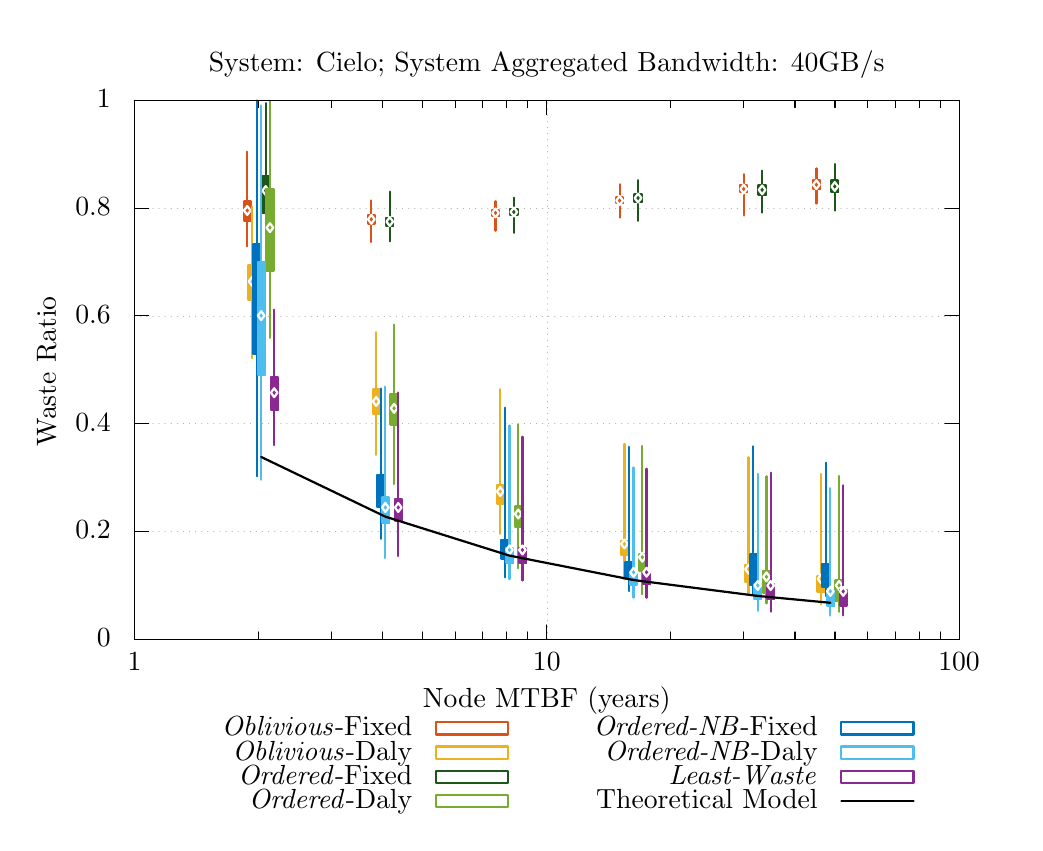
\begin{tikzpicture}[gnuplot]
%% generated with GNUPLOT 5.0p6 (Lua 5.3; terminal rev. 99, script rev. 100)
%% Thu Oct 19 16:09:22 2017
\path (0.000,0.000) rectangle (12.500,8.750);
\gpcolor{color=gp lt color axes}
\gpsetlinetype{gp lt axes}
\gpsetdashtype{gp dt axes}
\gpsetlinewidth{0.50}
\draw[gp path] (1.320,0.985)--(11.793,0.985);
\gpcolor{color=gp lt color border}
\gpsetlinetype{gp lt border}
\gpsetdashtype{gp dt solid}
\gpsetlinewidth{1.00}
\draw[gp path] (1.320,0.985)--(1.500,0.985);
\draw[gp path] (11.793,0.985)--(11.613,0.985);
\node[gp node right] at (1.136,0.985) {$0$};
\gpcolor{color=gp lt color axes}
\gpsetlinetype{gp lt axes}
\gpsetdashtype{gp dt axes}
\gpsetlinewidth{0.50}
\draw[gp path] (1.320,2.353)--(11.793,2.353);
\gpcolor{color=gp lt color border}
\gpsetlinetype{gp lt border}
\gpsetdashtype{gp dt solid}
\gpsetlinewidth{1.00}
\draw[gp path] (1.320,2.353)--(1.500,2.353);
\draw[gp path] (11.793,2.353)--(11.613,2.353);
\node[gp node right] at (1.136,2.353) {$0.2$};
\gpcolor{color=gp lt color axes}
\gpsetlinetype{gp lt axes}
\gpsetdashtype{gp dt axes}
\gpsetlinewidth{0.50}
\draw[gp path] (1.320,3.721)--(11.793,3.721);
\gpcolor{color=gp lt color border}
\gpsetlinetype{gp lt border}
\gpsetdashtype{gp dt solid}
\gpsetlinewidth{1.00}
\draw[gp path] (1.320,3.721)--(1.500,3.721);
\draw[gp path] (11.793,3.721)--(11.613,3.721);
\node[gp node right] at (1.136,3.721) {$0.4$};
\gpcolor{color=gp lt color axes}
\gpsetlinetype{gp lt axes}
\gpsetdashtype{gp dt axes}
\gpsetlinewidth{0.50}
\draw[gp path] (1.320,5.089)--(11.793,5.089);
\gpcolor{color=gp lt color border}
\gpsetlinetype{gp lt border}
\gpsetdashtype{gp dt solid}
\gpsetlinewidth{1.00}
\draw[gp path] (1.320,5.089)--(1.500,5.089);
\draw[gp path] (11.793,5.089)--(11.613,5.089);
\node[gp node right] at (1.136,5.089) {$0.6$};
\gpcolor{color=gp lt color axes}
\gpsetlinetype{gp lt axes}
\gpsetdashtype{gp dt axes}
\gpsetlinewidth{0.50}
\draw[gp path] (1.320,6.457)--(11.793,6.457);
\gpcolor{color=gp lt color border}
\gpsetlinetype{gp lt border}
\gpsetdashtype{gp dt solid}
\gpsetlinewidth{1.00}
\draw[gp path] (1.320,6.457)--(1.500,6.457);
\draw[gp path] (11.793,6.457)--(11.613,6.457);
\node[gp node right] at (1.136,6.457) {$0.8$};
\gpcolor{color=gp lt color axes}
\gpsetlinetype{gp lt axes}
\gpsetdashtype{gp dt axes}
\gpsetlinewidth{0.50}
\draw[gp path] (1.320,7.825)--(11.793,7.825);
\gpcolor{color=gp lt color border}
\gpsetlinetype{gp lt border}
\gpsetdashtype{gp dt solid}
\gpsetlinewidth{1.00}
\draw[gp path] (1.320,7.825)--(1.500,7.825);
\draw[gp path] (11.793,7.825)--(11.613,7.825);
\node[gp node right] at (1.136,7.825) {$1$};
\gpcolor{color=gp lt color axes}
\gpsetlinetype{gp lt axes}
\gpsetdashtype{gp dt axes}
\gpsetlinewidth{0.50}
\draw[gp path] (1.320,0.985)--(1.320,7.825);
\gpcolor{color=gp lt color border}
\gpsetlinetype{gp lt border}
\gpsetdashtype{gp dt solid}
\gpsetlinewidth{1.00}
\draw[gp path] (1.320,0.985)--(1.320,1.165);
\draw[gp path] (1.320,7.825)--(1.320,7.645);
\node[gp node center] at (1.320,0.677) {$1$};
\draw[gp path] (2.896,0.985)--(2.896,1.075);
\draw[gp path] (2.896,7.825)--(2.896,7.735);
\draw[gp path] (3.818,0.985)--(3.818,1.075);
\draw[gp path] (3.818,7.825)--(3.818,7.735);
\draw[gp path] (4.473,0.985)--(4.473,1.075);
\draw[gp path] (4.473,7.825)--(4.473,7.735);
\draw[gp path] (4.980,0.985)--(4.980,1.075);
\draw[gp path] (4.980,7.825)--(4.980,7.735);
\draw[gp path] (5.395,0.985)--(5.395,1.075);
\draw[gp path] (5.395,7.825)--(5.395,7.735);
\draw[gp path] (5.745,0.985)--(5.745,1.075);
\draw[gp path] (5.745,7.825)--(5.745,7.735);
\draw[gp path] (6.049,0.985)--(6.049,1.075);
\draw[gp path] (6.049,7.825)--(6.049,7.735);
\draw[gp path] (6.317,0.985)--(6.317,1.075);
\draw[gp path] (6.317,7.825)--(6.317,7.735);
\gpcolor{color=gp lt color axes}
\gpsetlinetype{gp lt axes}
\gpsetdashtype{gp dt axes}
\gpsetlinewidth{0.50}
\draw[gp path] (6.557,0.985)--(6.557,7.825);
\gpcolor{color=gp lt color border}
\gpsetlinetype{gp lt border}
\gpsetdashtype{gp dt solid}
\gpsetlinewidth{1.00}
\draw[gp path] (6.557,0.985)--(6.557,1.165);
\draw[gp path] (6.557,7.825)--(6.557,7.645);
\node[gp node center] at (6.557,0.677) {$10$};
\draw[gp path] (8.133,0.985)--(8.133,1.075);
\draw[gp path] (8.133,7.825)--(8.133,7.735);
\draw[gp path] (9.055,0.985)--(9.055,1.075);
\draw[gp path] (9.055,7.825)--(9.055,7.735);
\draw[gp path] (9.709,0.985)--(9.709,1.075);
\draw[gp path] (9.709,7.825)--(9.709,7.735);
\draw[gp path] (10.217,0.985)--(10.217,1.075);
\draw[gp path] (10.217,7.825)--(10.217,7.735);
\draw[gp path] (10.631,0.985)--(10.631,1.075);
\draw[gp path] (10.631,7.825)--(10.631,7.735);
\draw[gp path] (10.982,0.985)--(10.982,1.075);
\draw[gp path] (10.982,7.825)--(10.982,7.735);
\draw[gp path] (11.286,0.985)--(11.286,1.075);
\draw[gp path] (11.286,7.825)--(11.286,7.735);
\draw[gp path] (11.553,0.985)--(11.553,1.075);
\draw[gp path] (11.553,7.825)--(11.553,7.735);
\gpcolor{color=gp lt color axes}
\gpsetlinetype{gp lt axes}
\gpsetdashtype{gp dt axes}
\gpsetlinewidth{0.50}
\draw[gp path] (11.793,0.985)--(11.793,7.825);
\gpcolor{color=gp lt color border}
\gpsetlinetype{gp lt border}
\gpsetdashtype{gp dt solid}
\gpsetlinewidth{1.00}
\draw[gp path] (11.793,0.985)--(11.793,1.165);
\draw[gp path] (11.793,7.825)--(11.793,7.645);
\node[gp node center] at (11.793,0.677) {$100$};
\draw[gp path] (1.320,7.825)--(1.320,0.985)--(11.793,0.985)--(11.793,7.825)--cycle;
\node[gp node center,rotate=-270] at (0.246,4.405) {Waste Ratio};
\node[gp node center] at (6.556,0.215) {Node MTBF (years)};
\node[gp node center] at (6.556,8.287) {System: Cielo; System Aggregated Bandwidth: 40GB/s};
\node[gp node right] at (4.966,-0.149) {\propfixed};
\gpcolor{rgb color={0.851,0.325,0.098}}
\gpsetlinewidth{2.00}
\draw[gp path] (5.150,-0.226)--(6.066,-0.226)--(6.066,-0.072)--(5.150,-0.072)--cycle;
\gpfill{rgb color={0.851,0.325,0.098}} (2.708,6.295)--(2.798,6.295)--(2.798,6.541)--(2.708,6.541)--cycle;
\draw[gp path] (2.753,5.972)--(2.753,6.295);
\draw[gp path] (2.753,6.541)--(2.753,7.174);
\draw[gp path] (2.708,6.541)--(2.798,6.541)--(2.798,6.295)--(2.708,6.295)--cycle;
\gpfill{rgb color={0.851,0.325,0.098}} (4.284,6.263)--(4.374,6.263)--(4.374,6.370)--(4.284,6.370)--cycle;
\draw[gp path] (4.329,6.027)--(4.329,6.263);
\draw[gp path] (4.329,6.370)--(4.329,6.556);
\draw[gp path] (4.284,6.370)--(4.374,6.370)--(4.374,6.263)--(4.284,6.263)--cycle;
\gpfill{rgb color={0.851,0.325,0.098}} (5.861,6.363)--(5.951,6.363)--(5.951,6.437)--(5.861,6.437)--cycle;
\draw[gp path] (5.906,6.172)--(5.906,6.363);
\draw[gp path] (5.906,6.437)--(5.906,6.546);
\draw[gp path] (5.861,6.437)--(5.951,6.437)--(5.951,6.363)--(5.861,6.363)--cycle;
\gpfill{rgb color={0.851,0.325,0.098}} (7.437,6.519)--(7.527,6.519)--(7.527,6.593)--(7.437,6.593)--cycle;
\draw[gp path] (7.482,6.339)--(7.482,6.519);
\draw[gp path] (7.482,6.593)--(7.482,6.761);
\draw[gp path] (7.437,6.593)--(7.527,6.593)--(7.527,6.519)--(7.437,6.519)--cycle;
\gpfill{rgb color={0.851,0.325,0.098}} (9.013,6.658)--(9.103,6.658)--(9.103,6.754)--(9.013,6.754)--cycle;
\draw[gp path] (9.058,6.365)--(9.058,6.658);
\draw[gp path] (9.058,6.754)--(9.058,6.889);
\draw[gp path] (9.013,6.754)--(9.103,6.754)--(9.103,6.658)--(9.013,6.658)--cycle;
\gpfill{rgb color={0.851,0.325,0.098}} (9.936,6.701)--(10.026,6.701)--(10.026,6.813)--(9.936,6.813)--cycle;
\draw[gp path] (9.981,6.516)--(9.981,6.701);
\draw[gp path] (9.981,6.813)--(9.981,6.963);
\draw[gp path] (9.936,6.813)--(10.026,6.813)--(10.026,6.701)--(9.936,6.701)--cycle;
\gpcolor{rgb color={1.000,1.000,1.000}}
\gpsetpointsize{4.00}
\gppoint{gp mark 12}{(2.753,6.428)}
\gppoint{gp mark 12}{(4.329,6.316)}
\gppoint{gp mark 12}{(5.906,6.397)}
\gppoint{gp mark 12}{(7.482,6.554)}
\gppoint{gp mark 12}{(9.058,6.701)}
\gppoint{gp mark 12}{(9.981,6.756)}
\gpcolor{color=gp lt color border}
\node[gp node right] at (4.966,-0.457) {\propdaly};
\gpcolor{rgb color={0.929,0.694,0.125}}
\draw[gp path] (5.150,-0.534)--(6.066,-0.534)--(6.066,-0.380)--(5.150,-0.380)--cycle;
\gpfill{rgb color={0.929,0.694,0.125}} (2.769,5.296)--(2.859,5.296)--(2.859,5.740)--(2.769,5.740)--cycle;
\draw[gp path] (2.814,4.554)--(2.814,5.296);
\draw[gp path] (2.814,5.740)--(2.814,6.476);
\draw[gp path] (2.769,5.740)--(2.859,5.740)--(2.859,5.296)--(2.769,5.296)--cycle;
\gpfill{rgb color={0.929,0.694,0.125}} (4.345,3.847)--(4.435,3.847)--(4.435,4.156)--(4.345,4.156)--cycle;
\draw[gp path] (4.390,3.324)--(4.390,3.847);
\draw[gp path] (4.390,4.156)--(4.390,4.883);
\draw[gp path] (4.345,4.156)--(4.435,4.156)--(4.435,3.847)--(4.345,3.847)--cycle;
\gpfill{rgb color={0.929,0.694,0.125}} (5.921,2.708)--(6.011,2.708)--(6.011,2.943)--(5.921,2.943)--cycle;
\draw[gp path] (5.966,2.323)--(5.966,2.708);
\draw[gp path] (5.966,2.943)--(5.966,4.159);
\draw[gp path] (5.921,2.943)--(6.011,2.943)--(6.011,2.708)--(5.921,2.708)--cycle;
\gpfill{rgb color={0.929,0.694,0.125}} (7.498,2.053)--(7.588,2.053)--(7.588,2.233)--(7.498,2.233)--cycle;
\draw[gp path] (7.543,1.743)--(7.543,2.053);
\draw[gp path] (7.543,2.233)--(7.543,3.462);
\draw[gp path] (7.498,2.233)--(7.588,2.233)--(7.588,2.053)--(7.498,2.053)--cycle;
\gpfill{rgb color={0.929,0.694,0.125}} (9.074,1.712)--(9.164,1.712)--(9.164,1.922)--(9.074,1.922)--cycle;
\draw[gp path] (9.119,1.545)--(9.119,1.712);
\draw[gp path] (9.119,1.922)--(9.119,3.295);
\draw[gp path] (9.074,1.922)--(9.164,1.922)--(9.164,1.712)--(9.074,1.712)--cycle;
\gpfill{rgb color={0.929,0.694,0.125}} (9.996,1.579)--(10.086,1.579)--(10.086,1.785)--(9.996,1.785)--cycle;
\draw[gp path] (10.041,1.426)--(10.041,1.579);
\draw[gp path] (10.041,1.785)--(10.041,3.082);
\draw[gp path] (9.996,1.785)--(10.086,1.785)--(10.086,1.579)--(9.996,1.579)--cycle;
\gpcolor{rgb color={1.000,1.000,1.000}}
\gppoint{gp mark 12}{(2.814,5.528)}
\gppoint{gp mark 12}{(4.390,4.003)}
\gppoint{gp mark 12}{(5.966,2.859)}
\gppoint{gp mark 12}{(7.543,2.193)}
\gppoint{gp mark 12}{(9.119,1.873)}
\gppoint{gp mark 12}{(10.041,1.751)}
\gpcolor{color=gp lt color border}
\node[gp node right] at (4.966,-0.765) {\bfifofixed};
\gpcolor{rgb color={0.110,0.337,0.094}}
\draw[gp path] (5.150,-0.842)--(6.066,-0.842)--(6.066,-0.688)--(5.150,-0.688)--cycle;
\gpfill{rgb color={0.110,0.337,0.094}} (2.942,6.397)--(3.032,6.397)--(3.032,6.864)--(2.942,6.864)--cycle;
\draw[gp path] (2.987,6.053)--(2.987,6.397);
\draw[gp path] (2.987,6.864)--(2.987,7.790);
\draw[gp path] (2.942,6.864)--(3.032,6.864)--(3.032,6.397)--(2.942,6.397)--cycle;
\gpfill{rgb color={0.110,0.337,0.094}} (4.518,6.234)--(4.608,6.234)--(4.608,6.332)--(4.518,6.332)--cycle;
\draw[gp path] (4.563,6.037)--(4.563,6.234);
\draw[gp path] (4.563,6.332)--(4.563,6.668);
\draw[gp path] (4.518,6.332)--(4.608,6.332)--(4.608,6.234)--(4.518,6.234)--cycle;
\gpfill{rgb color={0.110,0.337,0.094}} (6.094,6.373)--(6.184,6.373)--(6.184,6.447)--(6.094,6.447)--cycle;
\draw[gp path] (6.139,6.145)--(6.139,6.373);
\draw[gp path] (6.139,6.447)--(6.139,6.590);
\draw[gp path] (6.094,6.447)--(6.184,6.447)--(6.184,6.373)--(6.094,6.373)--cycle;
\gpfill{rgb color={0.110,0.337,0.094}} (7.671,6.535)--(7.761,6.535)--(7.761,6.640)--(7.671,6.640)--cycle;
\draw[gp path] (7.716,6.297)--(7.716,6.535);
\draw[gp path] (7.716,6.640)--(7.716,6.812);
\draw[gp path] (7.671,6.640)--(7.761,6.640)--(7.761,6.535)--(7.671,6.535)--cycle;
\gpfill{rgb color={0.110,0.337,0.094}} (9.247,6.629)--(9.337,6.629)--(9.337,6.752)--(9.247,6.752)--cycle;
\draw[gp path] (9.292,6.402)--(9.292,6.629);
\draw[gp path] (9.292,6.752)--(9.292,6.935);
\draw[gp path] (9.247,6.752)--(9.337,6.752)--(9.337,6.629)--(9.247,6.629)--cycle;
\gpfill{rgb color={0.110,0.337,0.094}} (10.169,6.658)--(10.259,6.658)--(10.259,6.808)--(10.169,6.808)--cycle;
\draw[gp path] (10.214,6.428)--(10.214,6.658);
\draw[gp path] (10.214,6.808)--(10.214,7.018);
\draw[gp path] (10.169,6.808)--(10.259,6.808)--(10.259,6.658)--(10.169,6.658)--cycle;
\gpcolor{rgb color={1.000,1.000,1.000}}
\gppoint{gp mark 12}{(2.987,6.681)}
\gppoint{gp mark 12}{(4.563,6.287)}
\gppoint{gp mark 12}{(6.139,6.409)}
\gppoint{gp mark 12}{(7.716,6.586)}
\gppoint{gp mark 12}{(9.292,6.690)}
\gppoint{gp mark 12}{(10.214,6.733)}
\gpcolor{color=gp lt color border}
\node[gp node right] at (4.966,-1.073) {\bfifodaly};
\gpcolor{rgb color={0.467,0.675,0.188}}
\draw[gp path] (5.150,-1.150)--(6.066,-1.150)--(6.066,-0.996)--(5.150,-0.996)--cycle;
\gpfill{rgb color={0.467,0.675,0.188}} (2.996,5.660)--(3.086,5.660)--(3.086,6.697)--(2.996,6.697)--cycle;
\draw[gp path] (3.041,4.810)--(3.041,5.660);
\draw[gp path] (3.041,6.697)--(3.041,7.824);
\draw[gp path] (2.996,6.697)--(3.086,6.697)--(3.086,5.660)--(2.996,5.660)--cycle;
\gpfill{rgb color={0.467,0.675,0.188}} (4.573,3.711)--(4.663,3.711)--(4.663,4.102)--(4.573,4.102)--cycle;
\draw[gp path] (4.618,2.955)--(4.618,3.711);
\draw[gp path] (4.618,4.102)--(4.618,4.977);
\draw[gp path] (4.573,4.102)--(4.663,4.102)--(4.663,3.711)--(4.573,3.711)--cycle;
\gpfill{rgb color={0.467,0.675,0.188}} (6.149,2.408)--(6.239,2.408)--(6.239,2.668)--(6.149,2.668)--cycle;
\draw[gp path] (6.194,1.885)--(6.194,2.408);
\draw[gp path] (6.194,2.668)--(6.194,3.712);
\draw[gp path] (6.149,2.668)--(6.239,2.668)--(6.239,2.408)--(6.149,2.408)--cycle;
\gpfill{rgb color={0.467,0.675,0.188}} (7.725,1.856)--(7.815,1.856)--(7.815,2.059)--(7.725,2.059)--cycle;
\draw[gp path] (7.770,1.555)--(7.770,1.856);
\draw[gp path] (7.770,2.059)--(7.770,3.437);
\draw[gp path] (7.725,2.059)--(7.815,2.059)--(7.815,1.856)--(7.725,1.856)--cycle;
\gpfill{rgb color={0.467,0.675,0.188}} (9.302,1.575)--(9.392,1.575)--(9.392,1.849)--(9.302,1.849)--cycle;
\draw[gp path] (9.347,1.439)--(9.347,1.575);
\draw[gp path] (9.347,1.849)--(9.347,3.052);
\draw[gp path] (9.302,1.849)--(9.392,1.849)--(9.392,1.575)--(9.302,1.575)--cycle;
\gpfill{rgb color={0.467,0.675,0.188}} (10.224,1.465)--(10.314,1.465)--(10.314,1.729)--(10.224,1.729)--cycle;
\draw[gp path] (10.269,1.332)--(10.269,1.465);
\draw[gp path] (10.269,1.729)--(10.269,3.056);
\draw[gp path] (10.224,1.729)--(10.314,1.729)--(10.314,1.465)--(10.224,1.465)--cycle;
\gpcolor{rgb color={1.000,1.000,1.000}}
\gppoint{gp mark 12}{(3.041,6.210)}
\gppoint{gp mark 12}{(4.618,3.916)}
\gppoint{gp mark 12}{(6.194,2.574)}
\gppoint{gp mark 12}{(7.770,2.025)}
\gppoint{gp mark 12}{(9.347,1.776)}
\gppoint{gp mark 12}{(10.269,1.667)}
\gpcolor{color=gp lt color border}
\node[gp node right] at (10.114,-0.149) {\fifofixed};
\gpcolor{rgb color={0.000,0.447,0.741}}
\draw[gp path] (10.298,-0.226)--(11.214,-0.226)--(11.214,-0.072)--(10.298,-0.072)--cycle;
\gpfill{rgb color={0.000,0.447,0.741}} (2.828,4.608)--(2.918,4.608)--(2.918,5.997)--(2.828,5.997)--cycle;
\draw[gp path] (2.873,3.053)--(2.873,4.608);
\draw[gp path] (2.873,5.997)--(2.873,7.825);
\draw[gp path] (2.828,5.997)--(2.918,5.997)--(2.918,4.608)--(2.828,4.608)--cycle;
\gpfill{rgb color={0.000,0.447,0.741}} (4.404,2.667)--(4.494,2.667)--(4.494,3.073)--(4.404,3.073)--cycle;
\draw[gp path] (4.449,2.259)--(4.449,2.667);
\draw[gp path] (4.449,3.073)--(4.449,4.167);
\draw[gp path] (4.404,3.073)--(4.494,3.073)--(4.494,2.667)--(4.404,2.667)--cycle;
\gpfill{rgb color={0.000,0.447,0.741}} (5.980,2.009)--(6.070,2.009)--(6.070,2.241)--(5.980,2.241)--cycle;
\draw[gp path] (6.025,1.768)--(6.025,2.009);
\draw[gp path] (6.025,2.241)--(6.025,3.923);
\draw[gp path] (5.980,2.241)--(6.070,2.241)--(6.070,2.009)--(5.980,2.009)--cycle;
\gpfill{rgb color={0.000,0.447,0.741}} (7.557,1.770)--(7.647,1.770)--(7.647,1.961)--(7.557,1.961)--cycle;
\draw[gp path] (7.602,1.594)--(7.602,1.770);
\draw[gp path] (7.602,1.961)--(7.602,3.427);
\draw[gp path] (7.557,1.961)--(7.647,1.961)--(7.647,1.770)--(7.557,1.770)--cycle;
\gpfill{rgb color={0.000,0.447,0.741}} (9.133,1.676)--(9.223,1.676)--(9.223,2.060)--(9.133,2.060)--cycle;
\draw[gp path] (9.178,1.555)--(9.178,1.676);
\draw[gp path] (9.178,2.060)--(9.178,3.433);
\draw[gp path] (9.133,2.060)--(9.223,2.060)--(9.223,1.676)--(9.133,1.676)--cycle;
\gpfill{rgb color={0.000,0.447,0.741}} (10.055,1.652)--(10.145,1.652)--(10.145,1.939)--(10.055,1.939)--cycle;
\draw[gp path] (10.100,1.532)--(10.100,1.652);
\draw[gp path] (10.100,1.939)--(10.100,3.226);
\draw[gp path] (10.055,1.939)--(10.145,1.939)--(10.145,1.652)--(10.055,1.652)--cycle;
\gpcolor{color=gp lt color border}
\node[gp node right] at (10.114,-0.457) {\fifodaly};
\gpcolor{rgb color={0.302,0.745,0.933}}
\draw[gp path] (10.298,-0.534)--(11.214,-0.534)--(11.214,-0.380)--(10.298,-0.380)--cycle;
\gpfill{rgb color={0.302,0.745,0.933}} (2.885,4.342)--(2.975,4.342)--(2.975,5.777)--(2.885,5.777)--cycle;
\draw[gp path] (2.930,3.009)--(2.930,4.342);
\draw[gp path] (2.930,5.777)--(2.930,7.761);
\draw[gp path] (2.885,5.777)--(2.975,5.777)--(2.975,4.342)--(2.885,4.342)--cycle;
\gpfill{rgb color={0.302,0.745,0.933}} (4.462,2.459)--(4.552,2.459)--(4.552,2.782)--(4.462,2.782)--cycle;
\draw[gp path] (4.507,2.014)--(4.507,2.459);
\draw[gp path] (4.507,2.782)--(4.507,4.192);
\draw[gp path] (4.462,2.782)--(4.552,2.782)--(4.552,2.459)--(4.462,2.459)--cycle;
\gpfill{rgb color={0.302,0.745,0.933}} (6.038,1.951)--(6.128,1.951)--(6.128,2.143)--(6.038,2.143)--cycle;
\draw[gp path] (6.083,1.748)--(6.083,1.951);
\draw[gp path] (6.083,2.143)--(6.083,3.697);
\draw[gp path] (6.038,2.143)--(6.128,2.143)--(6.128,1.951)--(6.038,1.951)--cycle;
\gpfill{rgb color={0.302,0.745,0.933}} (7.614,1.679)--(7.704,1.679)--(7.704,1.830)--(7.614,1.830)--cycle;
\draw[gp path] (7.659,1.512)--(7.659,1.679);
\draw[gp path] (7.659,1.830)--(7.659,3.164);
\draw[gp path] (7.614,1.830)--(7.704,1.830)--(7.704,1.679)--(7.614,1.679)--cycle;
\gpfill{rgb color={0.302,0.745,0.933}} (9.191,1.494)--(9.281,1.494)--(9.281,1.679)--(9.191,1.679)--cycle;
\draw[gp path] (9.236,1.345)--(9.236,1.494);
\draw[gp path] (9.236,1.679)--(9.236,3.084);
\draw[gp path] (9.191,1.679)--(9.281,1.679)--(9.281,1.494)--(9.191,1.494)--cycle;
\gpfill{rgb color={0.302,0.745,0.933}} (10.113,1.408)--(10.203,1.408)--(10.203,1.604)--(10.113,1.604)--cycle;
\draw[gp path] (10.158,1.285)--(10.158,1.408);
\draw[gp path] (10.158,1.604)--(10.158,2.901);
\draw[gp path] (10.113,1.604)--(10.203,1.604)--(10.203,1.408)--(10.113,1.408)--cycle;
\gpcolor{rgb color={1.000,1.000,1.000}}
\gppoint{gp mark 12}{(2.930,5.093)}
\gppoint{gp mark 12}{(4.507,2.657)}
\gppoint{gp mark 12}{(6.083,2.118)}
\gppoint{gp mark 12}{(7.659,1.833)}
\gppoint{gp mark 12}{(9.236,1.666)}
\gppoint{gp mark 12}{(10.158,1.591)}
\gpcolor{color=gp lt color border}
\node[gp node right] at (10.114,-0.765) {\cooperative};
\gpcolor{rgb color={0.545,0.161,0.573}}
\draw[gp path] (10.298,-0.842)--(11.214,-0.842)--(11.214,-0.688)--(10.298,-0.688)--cycle;
\gpfill{rgb color={0.545,0.161,0.573}} (3.050,3.897)--(3.140,3.897)--(3.140,4.315)--(3.050,4.315)--cycle;
\draw[gp path] (3.095,3.448)--(3.095,3.897);
\draw[gp path] (3.095,4.315)--(3.095,5.168);
\draw[gp path] (3.050,4.315)--(3.140,4.315)--(3.140,3.897)--(3.050,3.897)--cycle;
\gpfill{rgb color={0.545,0.161,0.573}} (4.626,2.483)--(4.716,2.483)--(4.716,2.762)--(4.626,2.762)--cycle;
\draw[gp path] (4.671,2.040)--(4.671,2.483);
\draw[gp path] (4.671,2.762)--(4.671,4.116);
\draw[gp path] (4.626,2.762)--(4.716,2.762)--(4.716,2.483)--(4.626,2.483)--cycle;
\gpfill{rgb color={0.545,0.161,0.573}} (6.203,1.950)--(6.293,1.950)--(6.293,2.135)--(6.203,2.135)--cycle;
\draw[gp path] (6.248,1.730)--(6.248,1.950);
\draw[gp path] (6.248,2.135)--(6.248,3.554);
\draw[gp path] (6.203,2.135)--(6.293,2.135)--(6.293,1.950)--(6.203,1.950)--cycle;
\gpfill{rgb color={0.545,0.161,0.573}} (7.779,1.682)--(7.869,1.682)--(7.869,1.826)--(7.779,1.826)--cycle;
\draw[gp path] (7.824,1.510)--(7.824,1.682);
\draw[gp path] (7.824,1.826)--(7.824,3.147);
\draw[gp path] (7.779,1.826)--(7.869,1.826)--(7.869,1.682)--(7.779,1.682)--cycle;
\gpfill{rgb color={0.545,0.161,0.573}} (9.355,1.492)--(9.445,1.492)--(9.445,1.685)--(9.355,1.685)--cycle;
\draw[gp path] (9.400,1.333)--(9.400,1.492);
\draw[gp path] (9.400,1.685)--(9.400,3.099);
\draw[gp path] (9.355,1.685)--(9.445,1.685)--(9.445,1.492)--(9.355,1.492)--cycle;
\gpfill{rgb color={0.545,0.161,0.573}} (10.277,1.412)--(10.367,1.412)--(10.367,1.606)--(10.277,1.606)--cycle;
\draw[gp path] (10.322,1.286)--(10.322,1.412);
\draw[gp path] (10.322,1.606)--(10.322,2.938);
\draw[gp path] (10.277,1.606)--(10.367,1.606)--(10.367,1.412)--(10.277,1.412)--cycle;
\gpcolor{rgb color={1.000,1.000,1.000}}
\gppoint{gp mark 12}{(3.095,4.114)}
\gppoint{gp mark 12}{(4.671,2.656)}
\gppoint{gp mark 12}{(6.248,2.117)}
\gppoint{gp mark 12}{(7.824,1.834)}
\gppoint{gp mark 12}{(9.400,1.665)}
\gppoint{gp mark 12}{(10.322,1.590)}
\gpcolor{color=gp lt color border}
\node[gp node right] at (10.114,-1.073) {Theoretical Model};
\gpcolor{rgb color={0.000,0.000,0.000}}
\draw[gp path] (10.298,-1.073)--(11.214,-1.073);
\draw[gp path] (2.930,3.298)--(4.507,2.540)--(6.083,2.045)--(7.659,1.735)--(9.236,1.533)%
  --(10.158,1.446);
\gpcolor{color=gp lt color border}
\gpsetlinewidth{1.00}
\draw[gp path] (1.320,7.825)--(1.320,0.985)--(11.793,0.985)--(11.793,7.825)--cycle;
%% coordinates of the plot area
\gpdefrectangularnode{gp plot 1}{\pgfpoint{1.320cm}{0.985cm}}{\pgfpoint{11.793cm}{7.825cm}}
\end{tikzpicture}
%% gnuplot variables
}
  \end{center}
  \caption{Waste ratio as a function of the system MTBF for the
    seven I/O and Checkpointing scheduling strategies, and the LANL workload on
    Cielo. \label{fig:cielo-40gbs}}
\end{figure}

\paragraph{The Impact of System Reliability}
Next, we explore the performance of each approach under low bandwidth (and
thus high probability of interference). A scenario with such low bandwidth is not
unrealistic.  As shown in Luu et al~\cite{Luu:2015:Multiplatform}, practical
bandwidth can be considerably lower than theoretical.
Figure~\ref{fig:cielo-40gbs} represents the waste ratio on Cielo, assuming the
aggregated filesystem bandwidth of the system is 40GB/s. We vary the node MTBF
$\muind$ from 2 years (1h of system MTBF) to 50 years (24h of system MTBF) in
order to evaluate the impact of this parameter. Similar to
Figure~\ref{fig:cielo-1hmtbf}, we observe three classes of behavior: \propfixed
and \bfifofixed exhibit a waste ratio that remains constant around 80\% for all
values of the MTBF. These approaches are critically dependent on the filesystem
bandwidth, and a lower frequency of failures does not significantly improve
their performance. The I/O subsystem is saturated, and the applications spends
most of their time waiting for it.
%
\propdaly and \bfifodaly, see poor efficiency for small MTBF values, but
steadily improve to come close to the theoretical bound for higher MTBF values.
Lastly, \fifodaly, \fifofixed, and \cooperative quickly reach the theoretical
model performance, even with a low  MTBF (4 year node MTBF or 2h of
system MTBF).

For all the strategies that use the Daly checkpointing period, increasing the
MTBF reduces the amount of I/O required and thus relieves the pressure of a
constrained bandwidth. All strategies that schedule the bandwidth are
successful at increasing the efficiency close to the theoretical model.
%
Similarly, \fifofixed, despite its fixed checkpoint interval is capable of
reaching a performance comparable to the Daly-based strategies (which reduce the
number of total checkpoints). The rapid improvement of the \fifofixed approach can be
explained by a combination of 2 factors. Foremost, the non-blocking aspect of
the checkpoint provide the I/O subsystem with enough flexibility to order the
checkpoint without imposing an additional wait. Delayed checkpoints only translate
in additional waste if that application itself is subject to failure.
Additionally, for lower MTBFs, the more frequent restarts of interfering jobs,
despite the fact that they delay the checkpointing operation, do not introduce
additional waste.

%% HT + GB: we wanted to say the same thing but in a more clear setting
% Surprisingly so in the case of \fifofixed, with its fixed checkpoint
% interval, which is capable of reaching a performance
% comparable to the strategies that reduce the number of
% checkpoints. At 2h of system MTBF (4 years of node MTBF), the
% supplementary I/O from restarting processes competes with the high
% fixed checkpoint frequency for scarce I/O resources, resulting in
% significant wastage. However, at 8h of system MTBF (16 years of node
% MTBF), the number of restarts is greatly reduced and the non blocking
% checkpointing approach is sufficient to even the I/O load efficiently.

\subsection{Evaluating a Prospective System}

\begin{figure}
  \begin{center}
    \resizebox{1.05\linewidth}{!}{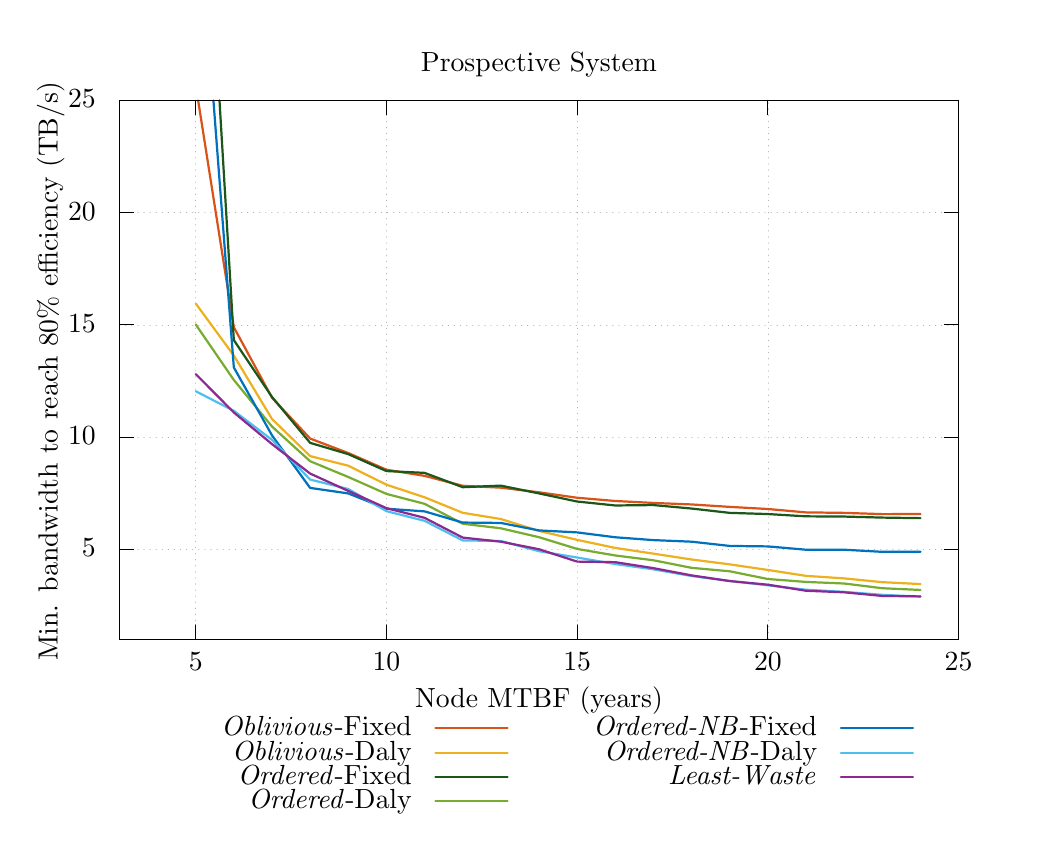
\begin{tikzpicture}[gnuplot]
%% generated with GNUPLOT 5.2p0 (Lua 5.3; terminal rev. 99, script rev. 102)
%% Thu Oct 19 14:13:35 2017
\path (0.000,0.000) rectangle (12.500,8.750);
\gpcolor{color=gp lt color axes}
\gpsetlinetype{gp lt axes}
\gpsetdashtype{gp dt axes}
\gpsetlinewidth{0.50}
\draw[gp path] (1.136,2.125)--(11.793,2.125);
\gpcolor{color=gp lt color border}
\gpsetlinetype{gp lt border}
\gpsetdashtype{gp dt solid}
\gpsetlinewidth{1.00}
\draw[gp path] (1.136,2.125)--(1.316,2.125);
\draw[gp path] (11.793,2.125)--(11.613,2.125);
\node[gp node right] at (0.952,2.125) {$5$};
\gpcolor{color=gp lt color axes}
\gpsetlinetype{gp lt axes}
\gpsetdashtype{gp dt axes}
\gpsetlinewidth{0.50}
\draw[gp path] (1.136,3.550)--(11.793,3.550);
\gpcolor{color=gp lt color border}
\gpsetlinetype{gp lt border}
\gpsetdashtype{gp dt solid}
\gpsetlinewidth{1.00}
\draw[gp path] (1.136,3.550)--(1.316,3.550);
\draw[gp path] (11.793,3.550)--(11.613,3.550);
\node[gp node right] at (0.952,3.550) {$10$};
\gpcolor{color=gp lt color axes}
\gpsetlinetype{gp lt axes}
\gpsetdashtype{gp dt axes}
\gpsetlinewidth{0.50}
\draw[gp path] (1.136,4.975)--(11.793,4.975);
\gpcolor{color=gp lt color border}
\gpsetlinetype{gp lt border}
\gpsetdashtype{gp dt solid}
\gpsetlinewidth{1.00}
\draw[gp path] (1.136,4.975)--(1.316,4.975);
\draw[gp path] (11.793,4.975)--(11.613,4.975);
\node[gp node right] at (0.952,4.975) {$15$};
\gpcolor{color=gp lt color axes}
\gpsetlinetype{gp lt axes}
\gpsetdashtype{gp dt axes}
\gpsetlinewidth{0.50}
\draw[gp path] (1.136,6.400)--(11.793,6.400);
\gpcolor{color=gp lt color border}
\gpsetlinetype{gp lt border}
\gpsetdashtype{gp dt solid}
\gpsetlinewidth{1.00}
\draw[gp path] (1.136,6.400)--(1.316,6.400);
\draw[gp path] (11.793,6.400)--(11.613,6.400);
\node[gp node right] at (0.952,6.400) {$20$};
\gpcolor{color=gp lt color axes}
\gpsetlinetype{gp lt axes}
\gpsetdashtype{gp dt axes}
\gpsetlinewidth{0.50}
\draw[gp path] (1.136,7.825)--(11.793,7.825);
\gpcolor{color=gp lt color border}
\gpsetlinetype{gp lt border}
\gpsetdashtype{gp dt solid}
\gpsetlinewidth{1.00}
\draw[gp path] (1.136,7.825)--(1.316,7.825);
\draw[gp path] (11.793,7.825)--(11.613,7.825);
\node[gp node right] at (0.952,7.825) {$25$};
\gpcolor{color=gp lt color axes}
\gpsetlinetype{gp lt axes}
\gpsetdashtype{gp dt axes}
\gpsetlinewidth{0.50}
\draw[gp path] (2.105,0.985)--(2.105,7.825);
\gpcolor{color=gp lt color border}
\gpsetlinetype{gp lt border}
\gpsetdashtype{gp dt solid}
\gpsetlinewidth{1.00}
\draw[gp path] (2.105,0.985)--(2.105,1.165);
\draw[gp path] (2.105,7.825)--(2.105,7.645);
\node[gp node center] at (2.105,0.677) {$5$};
\gpcolor{color=gp lt color axes}
\gpsetlinetype{gp lt axes}
\gpsetdashtype{gp dt axes}
\gpsetlinewidth{0.50}
\draw[gp path] (4.527,0.985)--(4.527,7.825);
\gpcolor{color=gp lt color border}
\gpsetlinetype{gp lt border}
\gpsetdashtype{gp dt solid}
\gpsetlinewidth{1.00}
\draw[gp path] (4.527,0.985)--(4.527,1.165);
\draw[gp path] (4.527,7.825)--(4.527,7.645);
\node[gp node center] at (4.527,0.677) {$10$};
\gpcolor{color=gp lt color axes}
\gpsetlinetype{gp lt axes}
\gpsetdashtype{gp dt axes}
\gpsetlinewidth{0.50}
\draw[gp path] (6.949,0.985)--(6.949,7.825);
\gpcolor{color=gp lt color border}
\gpsetlinetype{gp lt border}
\gpsetdashtype{gp dt solid}
\gpsetlinewidth{1.00}
\draw[gp path] (6.949,0.985)--(6.949,1.165);
\draw[gp path] (6.949,7.825)--(6.949,7.645);
\node[gp node center] at (6.949,0.677) {$15$};
\gpcolor{color=gp lt color axes}
\gpsetlinetype{gp lt axes}
\gpsetdashtype{gp dt axes}
\gpsetlinewidth{0.50}
\draw[gp path] (9.371,0.985)--(9.371,7.825);
\gpcolor{color=gp lt color border}
\gpsetlinetype{gp lt border}
\gpsetdashtype{gp dt solid}
\gpsetlinewidth{1.00}
\draw[gp path] (9.371,0.985)--(9.371,1.165);
\draw[gp path] (9.371,7.825)--(9.371,7.645);
\node[gp node center] at (9.371,0.677) {$20$};
\gpcolor{color=gp lt color axes}
\gpsetlinetype{gp lt axes}
\gpsetdashtype{gp dt axes}
\gpsetlinewidth{0.50}
\draw[gp path] (11.793,0.985)--(11.793,7.825);
\gpcolor{color=gp lt color border}
\gpsetlinetype{gp lt border}
\gpsetdashtype{gp dt solid}
\gpsetlinewidth{1.00}
\draw[gp path] (11.793,0.985)--(11.793,1.165);
\draw[gp path] (11.793,7.825)--(11.793,7.645);
\node[gp node center] at (11.793,0.677) {$25$};
\draw[gp path] (1.136,7.825)--(1.136,0.985)--(11.793,0.985)--(11.793,7.825)--cycle;
\node[gp node center,rotate=-270] at (0.276,4.405) {Min. bandwidth to reach 80\% efficiency (TB/s)};
\node[gp node center] at (6.464,0.215) {Node MTBF (years)};
\node[gp node center] at (6.464,8.287) {Prospective System};
\node[gp node right] at (4.966,-0.149) {\propfixed};
\gpcolor{rgb color={0.851,0.325,0.098}}
\gpsetlinewidth{2.00}
\draw[gp path] (5.150,-0.149)--(6.066,-0.149);
\draw[gp path] (2.136,7.825)--(2.589,4.946)--(3.074,4.050)--(3.558,3.532)--(4.042,3.348)%
  --(4.527,3.136)--(5.011,3.058)--(5.496,2.932)--(5.980,2.908)--(6.465,2.849)--(6.949,2.780)%
  --(7.433,2.739)--(7.918,2.714)--(8.402,2.695)--(8.887,2.664)--(9.371,2.637)--(9.855,2.594)%
  --(10.340,2.588)--(10.824,2.572)--(11.309,2.573);
\gpcolor{color=gp lt color border}
\node[gp node right] at (4.966,-0.457) {\propdaly};
\gpcolor{rgb color={0.929,0.694,0.125}}
\draw[gp path] (5.150,-0.457)--(6.066,-0.457);
\draw[gp path] (2.105,5.247)--(2.589,4.586)--(3.074,3.780)--(3.558,3.309)--(4.042,3.187)%
  --(4.527,2.946)--(5.011,2.786)--(5.496,2.589)--(5.980,2.510)--(6.465,2.359)--(6.949,2.245)%
  --(7.433,2.143)--(7.918,2.070)--(8.402,1.996)--(8.887,1.934)--(9.371,1.863)--(9.855,1.788)%
  --(10.340,1.756)--(10.824,1.708)--(11.309,1.684);
\gpcolor{color=gp lt color border}
\node[gp node right] at (4.966,-0.765) {\bfifofixed};
\gpcolor{rgb color={0.110,0.337,0.094}}
\draw[gp path] (5.150,-0.765)--(6.066,-0.765);
\draw[gp path] (2.407,7.825)--(2.589,4.782)--(3.074,4.060)--(3.558,3.477)--(4.042,3.334)%
  --(4.527,3.119)--(5.011,3.096)--(5.496,2.914)--(5.980,2.934)--(6.465,2.835)--(6.949,2.732)%
  --(7.433,2.682)--(7.918,2.687)--(8.402,2.643)--(8.887,2.588)--(9.371,2.573)--(9.855,2.544)%
  --(10.340,2.541)--(10.824,2.528)--(11.309,2.521);
\gpcolor{color=gp lt color border}
\node[gp node right] at (4.966,-1.073) {\bfifodaly};
\gpcolor{rgb color={0.467,0.675,0.188}}
\draw[gp path] (5.150,-1.073)--(6.066,-1.073);
\draw[gp path] (2.105,4.981)--(2.589,4.276)--(3.074,3.684)--(3.558,3.244)--(4.042,3.044)%
  --(4.527,2.829)--(5.011,2.703)--(5.496,2.450)--(5.980,2.392)--(6.465,2.279)--(6.949,2.130)%
  --(7.433,2.047)--(7.918,1.986)--(8.402,1.890)--(8.887,1.846)--(9.371,1.748)--(9.855,1.711)%
  --(10.340,1.691)--(10.824,1.631)--(11.309,1.609);
\gpcolor{color=gp lt color border}
\node[gp node right] at (10.114,-0.149) {\fifofixed};
\gpcolor{rgb color={0.000,0.447,0.741}}
\draw[gp path] (10.298,-0.149)--(11.214,-0.149);
\draw[gp path] (2.330,7.825)--(2.589,4.435)--(3.074,3.572)--(3.558,2.905)--(4.042,2.835)%
  --(4.527,2.641)--(5.011,2.607)--(5.496,2.465)--(5.980,2.460)--(6.465,2.365)--(6.949,2.340)%
  --(7.433,2.278)--(7.918,2.242)--(8.402,2.222)--(8.887,2.168)--(9.371,2.162)--(9.855,2.120)%
  --(10.340,2.120)--(10.824,2.093)--(11.309,2.094);
\gpcolor{color=gp lt color border}
\node[gp node right] at (10.114,-0.457) {\fifodaly};
\gpcolor{rgb color={0.302,0.745,0.933}}
\draw[gp path] (10.298,-0.457)--(11.214,-0.457);
\draw[gp path] (2.105,4.133)--(2.589,3.884)--(3.074,3.515)--(3.558,3.011)--(4.042,2.891)%
  --(4.527,2.610)--(5.011,2.487)--(5.496,2.238)--(5.980,2.231)--(6.465,2.101)--(6.949,2.021)%
  --(7.433,1.938)--(7.918,1.871)--(8.402,1.786)--(8.887,1.723)--(9.371,1.668)--(9.855,1.612)%
  --(10.340,1.585)--(10.824,1.547)--(11.309,1.525);
\gpcolor{color=gp lt color border}
\node[gp node right] at (10.114,-0.765) {\cooperative};
\gpcolor{rgb color={0.545,0.161,0.573}}
\draw[gp path] (10.298,-0.765)--(11.214,-0.765);
\draw[gp path] (2.105,4.351)--(2.589,3.863)--(3.074,3.461)--(3.558,3.087)--(4.042,2.867)%
  --(4.527,2.648)--(5.011,2.525)--(5.496,2.274)--(5.980,2.222)--(6.465,2.126)--(6.949,1.969)%
  --(7.433,1.962)--(7.918,1.886)--(8.402,1.794)--(8.887,1.722)--(9.371,1.676)--(9.855,1.599)%
  --(10.340,1.579)--(10.824,1.533)--(11.309,1.527);
\gpcolor{color=gp lt color border}
\gpsetlinewidth{1.00}
\draw[gp path] (1.136,7.825)--(1.136,0.985)--(11.793,0.985)--(11.793,7.825)--cycle;
%% coordinates of the plot area
\gpdefrectangularnode{gp plot 1}{\pgfpoint{1.136cm}{0.985cm}}{\pgfpoint{11.793cm}{7.825cm}}
\end{tikzpicture}
%% gnuplot variables
}
  \end{center}
  \caption{Minimum aggregated filesystem bandwidth to reach 80\%
    efficiency with the different approaches on the prospective
    future system.\label{fig:prosp}}
\end{figure}

In order to understand the impact of the I/O contention on future platforms, we
use our simulator to explore a prospective system and assess the impact of I/O
and checkpoint scheduling when the problem size and the machine size will
increase. We consider a future system with 7PB of main memory and 50,000
compute nodes (\eg Aurora\footnote{\url{https://aurora.alcf.anl.gov/}}). Based
on the APEX workflow report, we extrapolate the increase in problem size
expected for the application classes considered previously, and project these
applications on the prospective system.  We simulate the workload of
Table~\ref{table:lanl}, scaling the problem size proportionally to the change
in machine memory size. The waste is computed, as previously, by dividing the
amount of resource used for checkpoints and lost due to failures by the amount
of resource used in a fault-free and resilience-free run with the same initial
conditions.
%
We vary system MTBF; and for each strategy, we find the required aggregated
practical bandwidth necessary to provide a sustained 80\% efficiency of the
system.  This 80\% target efficiency is viewed by many programs (\eg 
The Exascale Computing Project\footnote{\url{https://exascaleproject.org}}) as a
reasonable cost for resilience activities.
%
Figure~\ref{fig:prosp} shows the impact of MTBF and strategies on this
prospective system.

When failures are frequent (less than 10 year node MTBF), the most critical
element is to reduce the I/O pressure: all strategies that use a fixed and
frequent checkpoint interval require greater available bandwidth to reach the
target efficiency.  In this case, strategies that combine an optimal
checkpointing period with I/O and checkpoint scheduling (\cooperative and
\fifodaly) perform similarly, consistently better than all other approaches.
These two approaches exhibit a strong resilience to failures, with a bandwidth
requirement that only increases by a factor of three between a very unstable system
(less than one hour system MTBF), and a stable one (an 8 hour system MTBF). In
contrast, the other strategies are much more dependent upon the frequency of
failures; the \propfixed strategy requires up to 50 times the bandwidth of
\cooperative to reach the same efficiency.

When failures are not endemic (\ie a node MTBF is at least 15 years
and a system MTBF of 2.6 hours), the hierarchy of different
approaches stabilizes. The two blocking strategies relying on
frequent checkpoints (\propfixed and \bfifofixed) remain expensive,
requiring the highest bandwidth to reach the target
efficiency. % 6.4TB/s at 24 years
The next contender, \fifofixed, requires a quarter of the  bandwidth
to reach the same efficiency.
% \fifofixed, that uses a fixed checkpoint interval comes next, with a
% requirement around three quarter of the one required by \propfixed and
% \bfifofixed.
Despite using the same fixed checkpoint interval as the previous methods, it
benefits from not blocking when the filesystem is not available.
This is sufficient, when failures are rare, to obtain a significant
performance gain. % 4.9TB/s at 24 years
All Daly-based strategies benefit from reduced I/O pressure, and reach the
target efficiency with around half the bandwidth needed by \propfixed. 
We also observe that \fifodaly and \leastwaste remain the most efficient strategies
for the whole MTBF spectrum. These
results highlight that checkpoint-based strategies can scale to
satisfy the need of future platforms, whether by integrating I/O-aware scheduling
strategies or by significantly over-provisioning the I/O partition.


% !TEX root =  ipdps18.tex

\section{Related Work}\label{sec:related}
% Primary: Kurt

We first discuss research regarding checkpoint-induced I/O pressure, followed by
works that regard avoiding I/O interference.  These techniques are not necessarily
independent: generally, reducing I/O pressure will reduce the likelihood of
interference.  Therefore, we focus our I/O interference discussion to those
techniques which consider the global scheduling of checkpoints and/or application I/O
across a platform.

%\todo[inline]{kbf: I am unsure about this breakdown.  These two things do not
%seem independent; reducing pressure seems to al reduce interference ...}

\paragraph*{Checkpointing and I/O}

For a single application, the Young/Daly formula~\cite{young74,daly04} gives the
optimal checkpointing period. This period minimizes platform waste, defined as the
fraction of job execution time that does not contribute to its progress.  The two
sources of waste are the time spent taking checkpoints (which motivates longer
checkpoint periods) and the time needed to recover and re-execute after each failure
(which motivates shorter checkpoint periods). The Young/Daly period achieves the
optimal trade-off between these sources to minimize the total waste. Arunagiri et
al.~\cite{Arunagiri2010} studied longer, sub-optimal periods with the intent of
reducing I/O pressure and showed, both analytically and empircally using four real
platforms, that a decrease in the I/O requirement can be achieved with only a small
increase in waste.

\paragraph*{Reducing I/O Pressure}

There are two general strategies for reducing I/O pressure from a single application:
hiding or reducing checkpoint commit times without reducing checkpoint data volumes,
and reducing commit times by reducing checkpoint data volumes.  Strategies that
attempt to hide checkpoint times include Diskless~\cite{Plank98Diskless} and remote
checkpoint protocols~\cite{Cornwell11RemoteBLCR} which leverage the typically higher
available bandwidths of the network or other storage media like RAM in order to
mitigate the performance of slower storage media like spinning or solid-state
disks. Additionally, remotely stored checkpoints have the additional benefit of
allowing systems to survive non-transient node failures. Similarly, multi-level
checkpoint protocols like SCR~\cite{Moody10SCR,Vaidya95TwoLevel} attempt to hide
checkpoint commit times by writing checkpoints to RAM, flash storage, or local disk
on the compute nodes~\cite{Kougkas2017} in addition to the parallel file system
thereby improving checkpoint or general I/O bandwidth.  Finally, checkpoint-specific
file systems like PLFS~\cite{Bent09PLFS} leverage the I/O patterns and
characteristics specific to checkpoint data to optimize checkpoint data transfers
to/from parallel file systems and therefore reduce checkpoint commit times.

Strategies that attempt to reduce checkpoint sizes include \emph{memory
exclusion}, which leverage user-directives or other hints to exclude portions of
process address spaces from checkpoints~\cite{Plank99MemoryExclusion}.
Additionally, incremental checkpointing protocols reduce checkpoint volumes by
utilizing the OS's memory page protection facilities to detect and save only
pages that have been updated between consecutive
checkpoints~\cite{Bronevetsky09Compiler,
Chen97CLIP,Elnozahy92ConsistentCheckpointing,Li94ConcurrentCheckpointing,
Plank94Libckpt,Paun10IncrementalWeibull,Kiswany08stdchk}.  Similarly,
page-based hashing techniques can also be used to avoid checkpointing pages
that have been written to but whose content has not
changed~\cite{Ferreira11Libhashckpt}.  Finally, compression-based techniques
use standard compression algorithms to reduce checkpoint
volumes~\cite{Ibtesham12Compression} and can be used at the
compiler-level~\cite{Li90CATCH} or in-memory~\cite{Plank94ICKP}.  Related,
Plank et al. proposed \textit{differential compression} to reduce checkpoint
sizes for incremental checkpoints~\cite{Plank95CompressedDiff} and Tanzima et
al.  show that similarities amongst checkpoint data from different processes
can be exploited to compress and reduce checkpoint data
volumes~\cite{tanzima12mcrengine}.  Finally, Sasaki et al propose a lossy
compression method based on wavelet transform and vector quantization to the
checkpoints of a production climate application~\cite{sasaki2015}, while Ni et
al~\cite{Ni2014} study the trade-offs between the loss of precision, compression
ratio, and application correctness due to lossy compression.

\paragraph*{Avoiding I/O interference}

Most closely related to our work, a number of studies have considered the global
scheduling of checkpoints and other I/O across a platform to reduce overall
congestion, thereby increasing performance.  Aupy et al.~\cite{Aupy:2017:Periodic}
presented a decentralized I/O scheduling technique for minimizing the congestion due
to checkpoint interference by taking advantage of the observed periodic and
deterministic nature of HPC application checkpoints and I/O.  This technique allows
the job scheduler to pre-define each application’s I/O behavior for their entire
execution.  Similarly, a number of works have investigated the efficiency of online
schedulers for data intensive~\cite{Groot2013,Sim:2015:AnalyzeThis} and HPC workload
I/O~\cite{Dorier2015,Gainaru:2016:Scheduling,Zhou:2015:IOAware,Herbein2017}.
Finally, a number of works have investigated utilizing recorded system reliability
information~\cite{Oliner:2006:Cooperative} and the statistical properties of these
failures~\cite{Tiwari:2014:Lazy} to determine effective checkpoint intervals for the
portion of the system used by the workload.

\paragraph*{Summary}

We distinguish our work from these previous studies in a number of important ways.
First, unlike a number of the previous studies, our technique considers existing
non-CR application I/O. Additionally, our approach is agnostic to the I/O patterns of
the considered applications as long as they are known.  Also, we attempt to optimize
the efficiency of the entire platform, with the changing workloads and failures
running on that platform, rather than just considering one workload. Finally and most
importantly, this approach provides optimal checkpointing periods in environments
where I/O is highly constrained and Daly/Young's formula is less appropriate, a common
scenario on many leadership-class systems.


%\section{Concluding Remarks}
\label{sec:conclusion}

In this paper we presented a comprehensive model to capture interference
between multiple applications performing fault-tolerance related I/O
on a shared HPC system. We proved that ... We designed multiple algorithms
to schedule and order the checkpointing I/O workload, with the intent of
diminishing the average slowdown sustained by applications on the
platform induced by sharing the I/O subsystem, \ie improve the throughput
of the platform. We designed a event-based simulator that permits
executing typical HPC workloads on current and prospective systems.
With this simulator we have been able to offer guidances as to the
prefered heuristics for scheduling checkpoint workloads, and the
general I/O requirements for future HPC systems to sustain checkpointing.
\section{Conclusion and Future Work} \label{sec:conclusion}
% Primary: Aurélien

As we design larger, likely more error-prone, platforms, effectively protecting
applications from platform faults becomes critical. Current fault-protection
techniques available on production platforms rely on checkpoint/restart to
ensure fault protection. However, these techniques, by their very nature,
regularly save the application state to stable storage, and therefore increase
the burden of the already overtaxed I/O subsystem.

Considering a comprehensive I/O interference model for platforms susceptible to I/O
contention, we designed multiple I/O scheduling algorithms that target improving
overall platform job throughput via waste minimization. We also theorized a
lower-bound for platform waste for I/O constrained checkpointing workloads. We use
this theoretical lower-bound to demonstrate the effectiveness of our \cooperative
I/O scheduling and to compare its performance with other I/O
scheduling strategies.  Our strategy invariably outperforms the others
with respect to the platform efficiency. Unsurprisingly, the biggest gains are
rendered on the platforms with a lowest MTBF or greater degrees of under-provisioned
I/O. Through simulation, we also show a path to supporting C/R on a prospective
system while maintaining 80\% platform efficiency, all without a large
investment in the I/O subsystem.

% In this paper we presented a comprehensive model to capture interference
% between multiple applications performing fault-tolerance related I/O
% on a shared HPC system. We designed multiple algorithms
% to schedule and order the checkpointing I/O workload, with the intent of
% diminishing the average slowdown sustained by applications on the
% platform induced by sharing the I/O subsystem, \ie improve the throughput
% of the platform. We formulated a steady-state analysis of a scenario
% where CR-CR interference is avoided, which helps us
% define a theoretical baseline for achievable performance in I/O
% constrained checkpointing workloads.
% We designed a event-based simulator that permits
% executing typical HPC workloads on current and prospective systems.
% With this simulator we have been able to demonstrate that our proposed
% heuristic improves the platform efficiency. Unsurprisingly the gain is
% more marked on platforms with a challenging MTBF or with
% under-provisioned I/O, but our heuristic improves the efficiency in
% all cases.  We also simulated the situation on a not yet available
% platform, this time with the goal of providing guidance in the
% general I/O requirements for future HPC systems to be able to
% sustain checkpointing with the desired 80\% efficiency, a goal that
% we have found achievable with a third of the I/O aggregate bandwidth
% requirements when the system employs a smart checkpointing policy.

As burst-buffers and other NVRAM storage mechanisms become more common, a natural
extension of this work would consider their impact on I/O contention/interference.
Increasing the available I/O
bandwidth leads to reduced waste (due to the decrease in checkpoint duration but also
an increase in the optimal checkpoint frequency and therefore a decrease in the
restart time), while providing relief to the shared I/O subsystem to better absorb
additional checkpoint information. We speculate that scheduling parallel filesystem
I/O with a heuristic that prioritizes jobs to minimize failure impact can help to
improve overall burst-buffer efficiencies. Such a heuristic would build upon the
strategies discussed in this work and extend them to the new framework.

% As burst-buffers and other NVRAM storage are becoming more common
% in PFS architecting, a natural extension of this work is to consider the effect
% of I/O contention/interference with hierarchies, in which subgroups of
% nodes (\eg a cabinet) may share a burst buffer, and thus experience
% interference for I/O in that same group, but be immune to interferences
% from I/O from other groups. Another interesting point with burst-buffers,
% is that space availability, in addition to bandwidth, may become
% contentious. The speed at which the burst-buffers can be committed to
% the sink PFS (possibly creating interference between multiple burst-buffers being
% flushed to the sink PFS simultaneously) now interplays with the
% optimal checkpoint frequency of applications, and can cause some
% applications running out of burst-buffer space. Again, we postulate that
% scheduling the commits to the PFS sink with an heuristic that prioritizes
% applications whose loss in failure cases would be more costly
% can play a role in improving the efficiency of the whole burst-buffers
% system.

%\section*{Acknowledgement}


\bibliographystyle{IEEEtran}
\bibliography{biblio}

%
%%%%%%%%%%%%%%%%%%%%%%%%%%%%%%%%%%%%%%%%%%%%%%%%%%%%%%%%%%%%%%%%%%%%%%%%
% FOLLOWUP TEXT IS OLDER AND MAY NEED MERGING OR DISCARDING
%%%%%%%%%%%%%%%%%%%%%%%%%%%%%%%%%%%%%%%%%%%%%%%%%%%%%%%%%%%%%%%%%%%%%%%%

\newpage
\appendix

\section{Older text}





\section{Optimal Cooperative Checkpointing Strategy}
\label{sec.strategy}

\subsection{With Burst Buffers}

We slightly change the machine model, and will consider that, in addition
to the global PFS, each node is provisioned with a local stage-in I/O
burst buffer. With burst buffers, $\ckpt{i}$ still represents the time it
takes to upload the checkpoint to the stable storage (the file system).
However, the availability of burst buffers permits a reduction in the
apparent time for the checkpoints as experienced by application idle
time. Note that under I/O constraints on the PFS, checkpoints may remain
in burst buffers (which is not a stable storage) until sufficient
PFS bandwidth is available.

Consider Algorithm~\ref{alg.withbb}: every $\period{i}$ time
units, each application of class $\app{i}$ takes a checkpoint and save
it onto the next free slot on the burst buffer; a global shared FIFO
queue transfers checkpoints from active slots in burst buffers onto
the parallel file system following the FIFO queue order.

\algblockdefx{Process}{EndProcess}[1]{\textbf{On Process} #1}{\textbf{End Process}}
\algnotext{EndProcess}
\algblockdefx{Every}{DoneEvery}[1]{\textbf{Every } #1}{\textbf{Done}}
\algnotext{DoneEvery}
\algblockdefx{When}{DoneWhen}[1]{\textbf{When } #1}{\textbf{Done}}
\algnotext{DoneWhen}
\algloopdefx{If}[1]{\textbf{If} #1 \textbf{then}}
\begin{algorithm}
\caption{Cooperative Checkpointing Algorithm with Burst Buffers}
\label{alg.withbb}
\begin{algorithmic}
\State \textbf{var} $transfer\_queue$, a FIFO initially empty
\Process{$p$, belonging to application $\application{i}{j}$ of class $\app{i}$}
   \State \textbf{var} $slots$ set of burst buffer files that can
   store a checkpoint
   \Every{$\period{i}$ time units}
           \State $slot  \gets $ oldest slot that is not being used for transfer
           \State Checkpoint application state into $slot$
           \If{$slot$ is marked done transferring}
                  \State Append $(p, slot)$ to $transfer\_queue$
    \DoneEvery
\EndProcess

\Process{$T$}
   \When{$transfer\_queue$ is not empty}
       \State Pop $slot$ from $transfer\_queue$
       \State Mark $slot$ as being transferred
       \State Transfer Checkpoint in $slot$ to File System
       \State Mark $slot$ as done transferring
   \DoneWhen
\EndProcess
\end{algorithmic}
\end{algorithm}

\begin{theorem}
  Algorithm~\ref{alg.withbb} ensures that all applications of class $\app{i}$
  checkpoint at most every $max(\sum_j\nbapp{j}*\ckpt{j}, \period{i})$
  time units, and requires only a burst buffer capable of storing 2
  checkpoints per process.
\end{theorem}

\begin{proof}
  \todo{This derives from $\sum_i \frac{\ckpt{i}}{\period{i}} \leq 1$,
    but should be done properly.}
\end{proof}

The theorem does provide a lower bound for the platform waste.\todo[inline]{the 2 storages holds only after the optimization, doesn't it? Or is it also a consequence of the above "proof" sketch?}
However, we have a FIFO system, and some applications may incur
a re-execution time larger than $P_{i}$. What is the worst case?
A first optimization is the following: when a checkpoint is taken
    by a given application, we check whether its previous checkpoint is
    still in the queue from the burst buffer to the file system. If yes, the new
checkpoint should \emph{replace} the old one, keeping the same position in the queue.
With this optimization, there is at most two checkpoints per application in the queue,
one being currently transferred and one waiting.
Then the worst case is to wait for the checkpoint of all the other applications.
Formally, the maximal re-execution time for application
$\application{i}{j}$ of class
$\app{i}$ is
$$\max(P_{i}, \sum_{k=1}^{\nbapps} n_{k}C_{k} - C_{i})$$

 \todo[inline]{Discussed at JLESC meeting: size of burst buffer can be
    bounded by 2 checkpoints easily, and it should be: if there are 3
    checkpoints in the burst buffer, then the first one might be being
    transferred, but this means that the 2nd is useless as we already
    reached the 3rd one. The 2nd should be discarded and its slot in
    the FIFO queue should be taken by the 3rd.}

  \todo[inline]{No clear what qualifies for burst buffers here, but
    currently the NVM bandwidth is (1) significantly lower than the
    network bandwidth, and (2) unidirectional. This might change in
    the future, but at least today it seems cheaper to use a
    buddy-checkpointing approach.}%


\subsection{Without Burst Buffers}

Without a local caching mechanism\footnote{Note that this case covers ``shared'' burst-buffers, where the
PFS contains an intermediate stage-in area (presumably with SSD drives, a much higher bandwidth, and possibly contention reduced to a subset of the nodes it serves, but provides for stable/persistent storage as soon as the data is committed to the shared burst-buffer.}, the times at which to take the checkpoint
must be scheduled to avoid any kind of checkpoint-checkpoint
interference (which can only waste resources, as all interfering
applications are slowed down while blocking on non-productive
operations). We consider here a centralized scheduler that decides at
any time what next application should checkpoint, and when.

The scheduler remembers when each application $\application{i}{j}$ of class
$\app{i}$ last initiated a checkpoint. We then define $\lastckpt{i}{j}$
as the time since the last checkpoint $\application{i}{j}$ started
(or since the start of $\application{i}{j}$ if none has been taken yet).
As soon as $\application{i}{j}$ has executed for $P_{i}$ time-units,
it is put in the checkpointing pool $\pool$ by the centralized scheduler. It
continues executing until it is selected from the pool to checkpoint.

Which application in the pool should be selected to checkpoint?
Assume that some previous checkpoint terminates at time $t$,
and let
$$\pool = \{ \application{i_{1}}{j_{1}}, \dots, \application{i_{k}}{j_{k}} \}$$
be the set of applications  in the pool at time $t$. All these applications are
candidate to checkpointing. At time $t$, each application $\application{i_{\ell}}{j_{\ell}} \in \pool$
has been executing for  $\lastckpt{i_{\ell}}{j_{\ell}}$ time-units.

If we select $\application{i_{\ell}}{j_{\ell}}$ to checkpoint (in time $C_{j_{\ell}}$),
and if there is a failure during that checkpoint, the time lost by every other application
$\application{i_{m}}{j_{m}} \in \pool$, $m \neq \ell$, is (in expectation) equal to
 $\lastckpt{i_m}{j_m} + \frac{C_{j_{\ell}}}{2}$.
We define the risk incurred by application
$\application{i_{m}}{j_{m}} \in \pool$, $m \neq \ell$
as its potential waste, which is the time lost divided by its MTBF $\frac{\mtbfplat}{\nbnodes{i}}$,
times the number $\nbnodes{i_m}$ processors enrolled by this application, i.e.
$$ \frac{\nbnodes{i_{m}}}{\mtbfplat}  (\lastckpt{i_m}{j_m} + \frac{C_{j_{\ell}}}{2})
\times \nbnodes{i_m} $$
Altogether, selecting $\application{i_{\ell}}{j_{\ell}}$ to checkpoint leads to a total risk
$$\risk(\application{i_{\ell}}{j_{\ell}}) = \sum_{1 \leq m \leq k, m \neq \ell} \frac{\nbnodes{i_{m}}^{2}}{\mtbfplat}  \times (\lastckpt{i_m}{j_m} + \frac{C_{j_{\ell}}}{2})$$
  for all applications that stayed in the pool.

We greedily choose the application in the pool that minimizes the risk:
$$\application{i_{\ell}}{j_{\ell}} = Argmin_{\application{i_m}{j_m} \in \pool} \risk(\application{i_m}{j_m})$$

%At the end of each checkpointing, the scheduler selects
%$\application{i}{j}$ such that
%$$
%\left\{
%\begin{array}{l}
%\nbnodes{i}(\frac{\wastefct{i}{\lastckpt{i}{j}}}{\wastefct{i}{\period{i}}}) \textrm{ if }\lastckpt{i}{j}\geq\period{i}\\
%0\textrm{ if }\lastckpt{i}{j}<\period{i}\\
%\end{array}\right.$$
%is maximal and strictly superior to 0.

Two remarks:
\begin{itemize}
\item Because we put applications in the pool only after they have run for $P_{i}$ times-steps,
this greedy algorithm guarantees Young/Daly periods to every application
whenever there is non conflict to access I/O resources.
\item The final schedule is not periodic. Instead, it is constructed dynamically
after each checkpoint completion. Computing the actual waste can be achieved
through simulation, and compared to the lower bound of Section~\ref{sec.optimal}.
\end{itemize}


\end{document}
